\documentclass[12pt,a4paper,titlepage,listof=totoc,bibliography=totoc,chapteratlists=0pt]{scrreprt}

\begin{filecontents*}{\jobname.xmpdata}
	\Keywords{VR, IOT, TODO}
	\Title{Unser tolles Thema -- wir sind suppa}
	\Author{Stefan Schwammal, Susi Schwammal}
\end{filecontents*}

\setcounter{tocdepth}{1}

% \usepackage{svg}
\usepackage[utf8]{inputenc}
\usepackage[T1]{fontenc}
\usepackage{amsmath}
\usepackage{amsfonts}
\usepackage{amssymb}
\usepackage[table]{xcolor}
\usepackage{graphicx}
\usepackage{caption}
\usepackage[left=3.50cm, right=2.00cm, top=2.00cm, bottom=2.00cm,foot=1cm]{geometry}
\usepackage[splitrule,hang,flushmargin,multiple,bottom]{footmisc}
\usepackage{lmodern, textcomp}
\usepackage{lmodern}
\usepackage{pdfpages}
\usepackage[ngerman]{babel}
\usepackage{multicol}
\usepackage{subfig}
\usepackage{float}
\usepackage{array,tabularx,booktabs}
\usepackage{ragged2e}
\usepackage{lipsum}
\usepackage{wrapfig}
% \usepackage{float}

% add tblr 



\newcolumntype{M}[1]{>{\centering\arraybackslash}m{#1}}

\usepackage{enumitem}
\newlist{compactitem}{itemize}{3}
\setlist[compactitem,1]{label=\textbullet, nosep,leftmargin=1.5em,labelwidth=*,align=left}
\setlist[compactitem,2]{label=--, nosep,leftmargin=1.5em,labelwidth=*,align=left}
\setlist[compactitem,3]{label=\textopenbullet, nosep,leftmargin=1.5em,labelwidth=*,align=left}
\newlist{compactenum}{enumerate}{3}
\setlist[compactenum,1]{label=\arabic*., nosep,leftmargin=1.5em,labelwidth=*,align=left}
\setlist[compactenum,2]{label=\alph*., nosep,leftmargin=1.5em,labelwidth=*,align=left}
\setlist[compactenum,3]{label=\roman*., nosep,leftmargin=1.5em,labelwidth=*,align=left}
\newlist{compactdesc}{description}{3}
\setlist[compactdesc]{leftmargin=1.5em,labelwidth=*,align=left}

\usepackage{microtype}

\usepackage[parfill]{parskip}

\definecolor{bluekeywords}{rgb}{0.13,0.13,1}
\definecolor{greencomments}{rgb}{0,0.5,0}
\definecolor{redstrings}{rgb}{0.9,0,0}
\definecolor{lightgray}{gray}{0.9}
\definecolor{lightblue}{rgb}{0.93,0.95,1.0}

\usepackage{listings}

\makeatletter
\lstdefinestyle{lststyle}{
	basicstyle=%
	\ttfamily
	\lst@ifdisplaystyle\scriptsize\fi
}
\makeatother

\renewcommand{\lstlistlistingname}{List of Listings}
% TODO: define other languages as needed
\lstset{language=Python,
	numbers=left,
	numberstyle=\tiny,
	showspaces=false,
	showtabs=false,
	breaklines=true,
	lineskip=-1pt,
	tabsize=2,
	showstringspaces=false,
	breakatwhitespace=true,
	escapeinside={(*@}{@*)},
	commentstyle=\color{greencomments},
	keywordstyle=\color{bluekeywords}\bfseries,
	stringstyle=\color{redstrings},
	style=lststyle,
	xleftmargin=17pt,
	framexleftmargin=17pt,
	framexrightmargin=5pt,
	framexbottommargin=4pt
}
\lstset{
	morekeywords={base,var,in,out,dynamic,from,where,select,orderby,function,\$,group,by,into,yield,async,await,@,None,self,as,elif,with}
}
\lstdefinelanguage{TypeScript}{
	keywords={typeof, new, true, false, catch, function, return, null, switch, var, if, in, while, do, else, case, break, void, number, string, boolean, module, \$, export, for, this},
	keywordstyle=\color{blue}\bfseries,
	ndkeywords={class, export, boolean, throw, implements, import, this},
	ndkeywordstyle=\color{darkgray}\bfseries,
	identifierstyle=\color{black},
	sensitive=false,
	comment=[l]{//},
	morecomment=[s]{/*}{*/},
	commentstyle=\color{purple}\ttfamily,
	stringstyle=\color{red}\ttfamily,
	morestring=[b]',
	morestring=[b]"
}
\usepackage{caption}
\DeclareCaptionFont{white}{\color{white}}
\DeclareCaptionFormat{listing}{\colorbox[cmyk]{0.43, 0.35, 0.35,0.01}{\parbox{\textwidth}{\hspace{10pt}#1#2#3}}}
\captionsetup[lstlisting]{format=listing,labelfont=white,textfont=white}
\captionsetup[table]{justification=centering, singlelinecheck=false}

\usepackage{setspace}
\newcommand{\MSonehalfspacing}{%
	\setstretch{1.44}%  default
	\ifcase \@ptsize \relax % 10pt
		\setstretch {1.448}%
	\or % 11pt
		\setstretch {1.399}%
	\or % 12pt
		\setstretch {1.433}%
	\fi
}

\newcommand{\setauthor}[1]{\ohead[]{#1}}

\usepackage[automark]{scrlayer-scrpage}
\pagestyle{scrheadings}
\automark{chapter}
\renewcommand\sectionmark[1]{\markright{\MakeMarkcase {\thesection\hskip .5em\relax#1}}}
\rohead{\ifnum\expandafter\pdfstrcmp\botmark=0 \rightmark\else\leftmark{} --- \rightmark\fi}
\ihead[]{\headmark}
\chead[]{}
\ohead{}
\cfoot[]{}
\ofoot[\pagemark]{\pagemark}
\setheadsepline{.1pt}

\usepackage[hyphens]{url}

\usepackage[a-1b]{pdfx}

\usepackage{hyperref}
\hypersetup{pdfa}

\usepackage[nonumberlist,toc,nopostdot]{glossaries}

\usepackage{chngcntr}
\counterwithout{footnote}{chapter}
\counterwithout{figure}{chapter}
\counterwithout{table}{chapter}
\AtBeginDocument{
	\counterwithout{lstlisting}{chapter}
	\urlstyle{sf}
}
\newcounter{RPages}



\makeatletter
\def\bstctlcite{\@ifnextchar[{\@bstctlcite}{\@bstctlcite[@auxout]}}
\def\@bstctlcite[#1]#2{\@bsphack
	\@for\@citeb:=#2\do{%
		\edef\@citeb{\expandafter\@firstofone\@citeb}%
		\if@filesw\immediate\write\csname #1\endcsname{\string\citation{\@citeb}}\fi}%
	\@esphack}
\makeatother

\clubpenalty=10000
\widowpenalty=10000
\displaywidowpenalty=10000
\interfootnotelinepenalty=10000

\title{Unser tolles Thema -- wir sind suppa}
\author{Stefan Schwammal, Susi Schwammal}

\makeindex
\makeglossaries
\begin{document}
\bstctlcite{IEEEexample:BSTcontrol}
\newcommand{\reminder}[1]
{ \textcolor{red}{<[{\bf\marginpar{\mbox{$<==$}} #1 }]>} }
\newcommand{\icode}[1]{\lstinline$#1$}
%\urlstyle{same}
%\setstretch{1.5}
\setstretch {1.433}
\renewcommand{\arraystretch}{1.2}

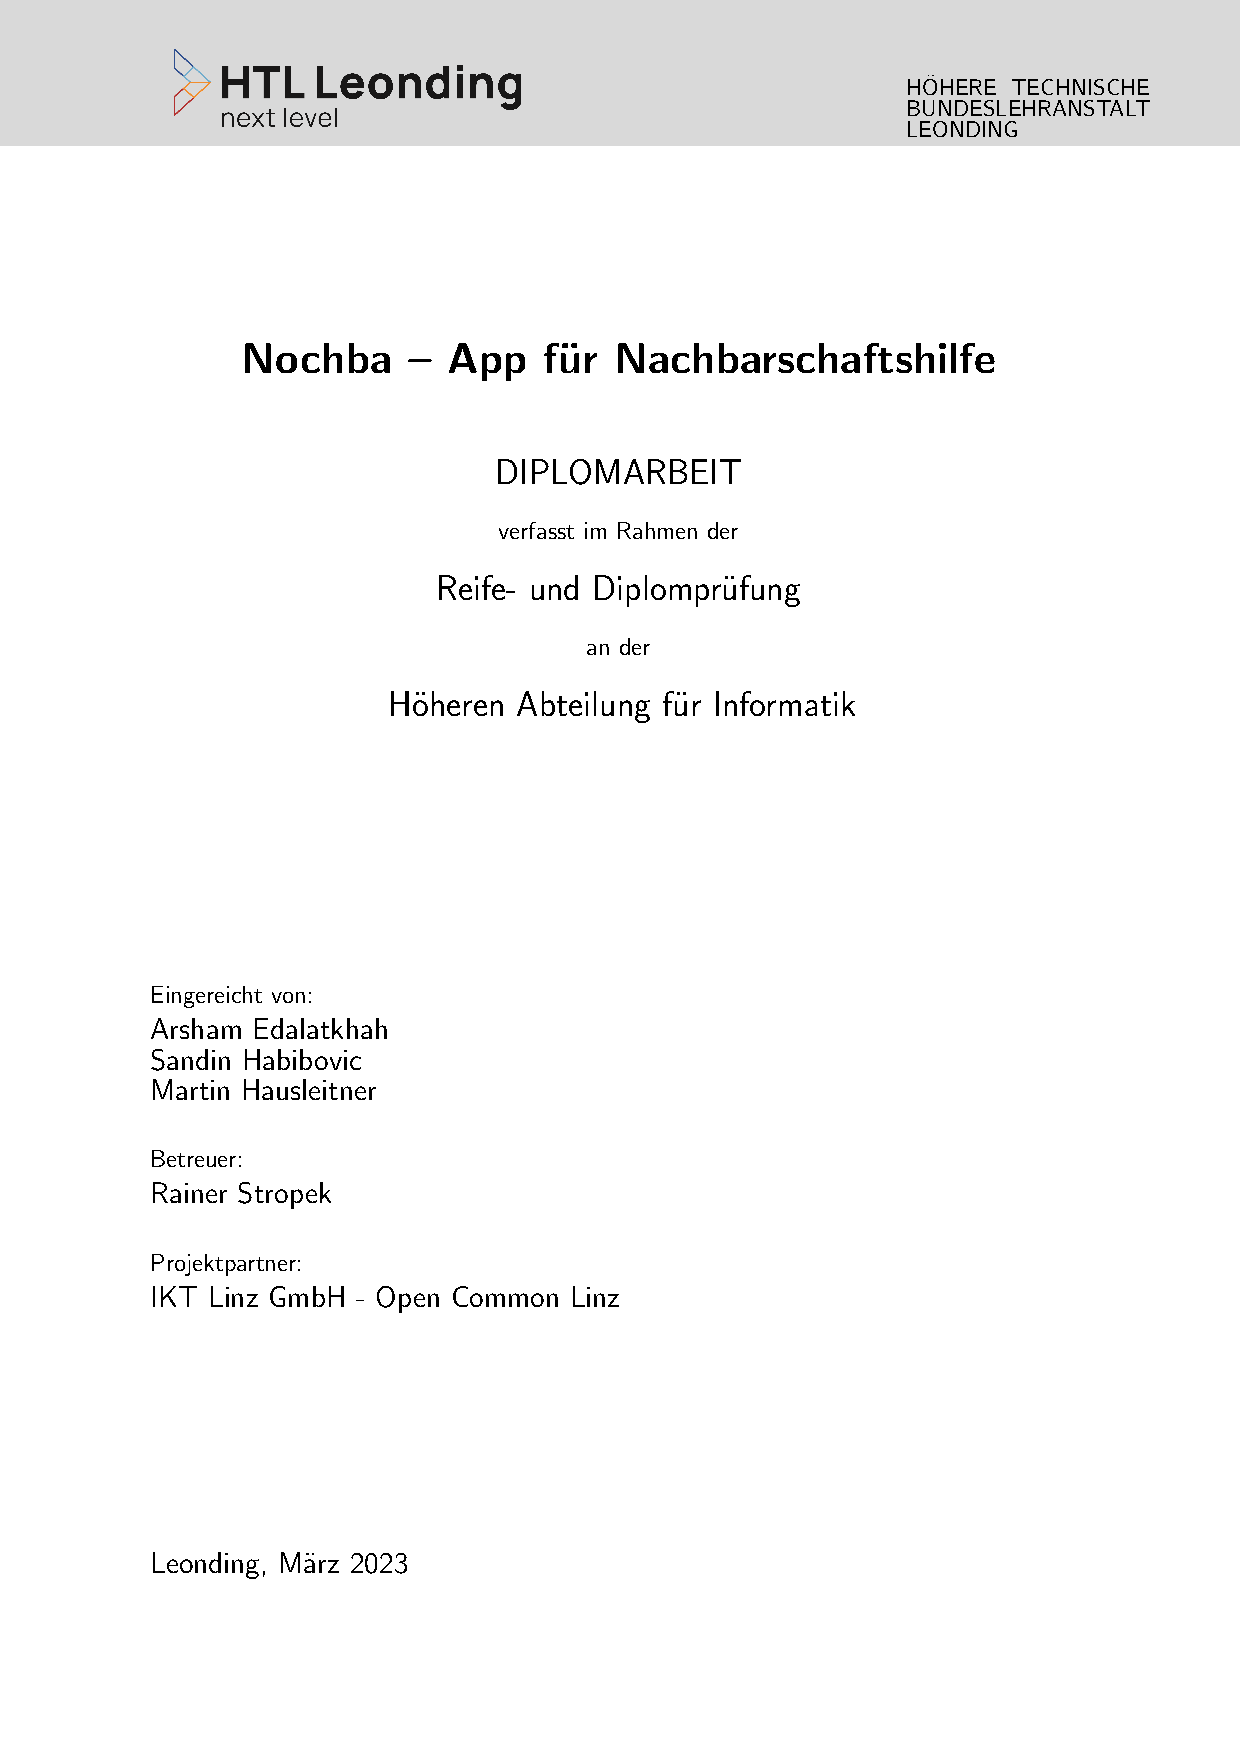
\includepdf{./titlepage/coversheet}
\pagenumbering{Roman}
\newpage
\thispagestyle{empty}
\vspace{3cm}
~ \\ \\
Ich erkläre an Eides statt, dass ich die vorliegende Diplomarbeit selbstständig und ohne fremde Hilfe verfasst, andere als die angegebenen Quellen und Hilfsmittel nicht benutzt bzw. die wörtlich oder sinngemäß entnommenen Stellen als solche kenntlich gemacht habe.

Die Arbeit wurde bisher in gleicher oder ähnlicher Weise keiner anderen Prüfungsbehörde vorgelegt und auch noch nicht veröffentlicht.

Die vorliegende Diplomarbeit ist mit dem elektronisch übermittelten Textdokument identisch.
\vspace{3cm}
% Hier kommt die Unterschrift drüber
\begin{tabbing}
    Leonding, März 2023 \hspace{3cm} A. Edalatkhah \& S. Habibovic \& M. Hausleitner
\end{tabbing}
\vspace{10cm}
\newpage
\setcounter{page}{1}

\begin{spacing}{1}
  \chapter*{Abstract}
\end{spacing}
\begin{wrapfigure}{r}{0.3\textwidth}
  \begin{center}
    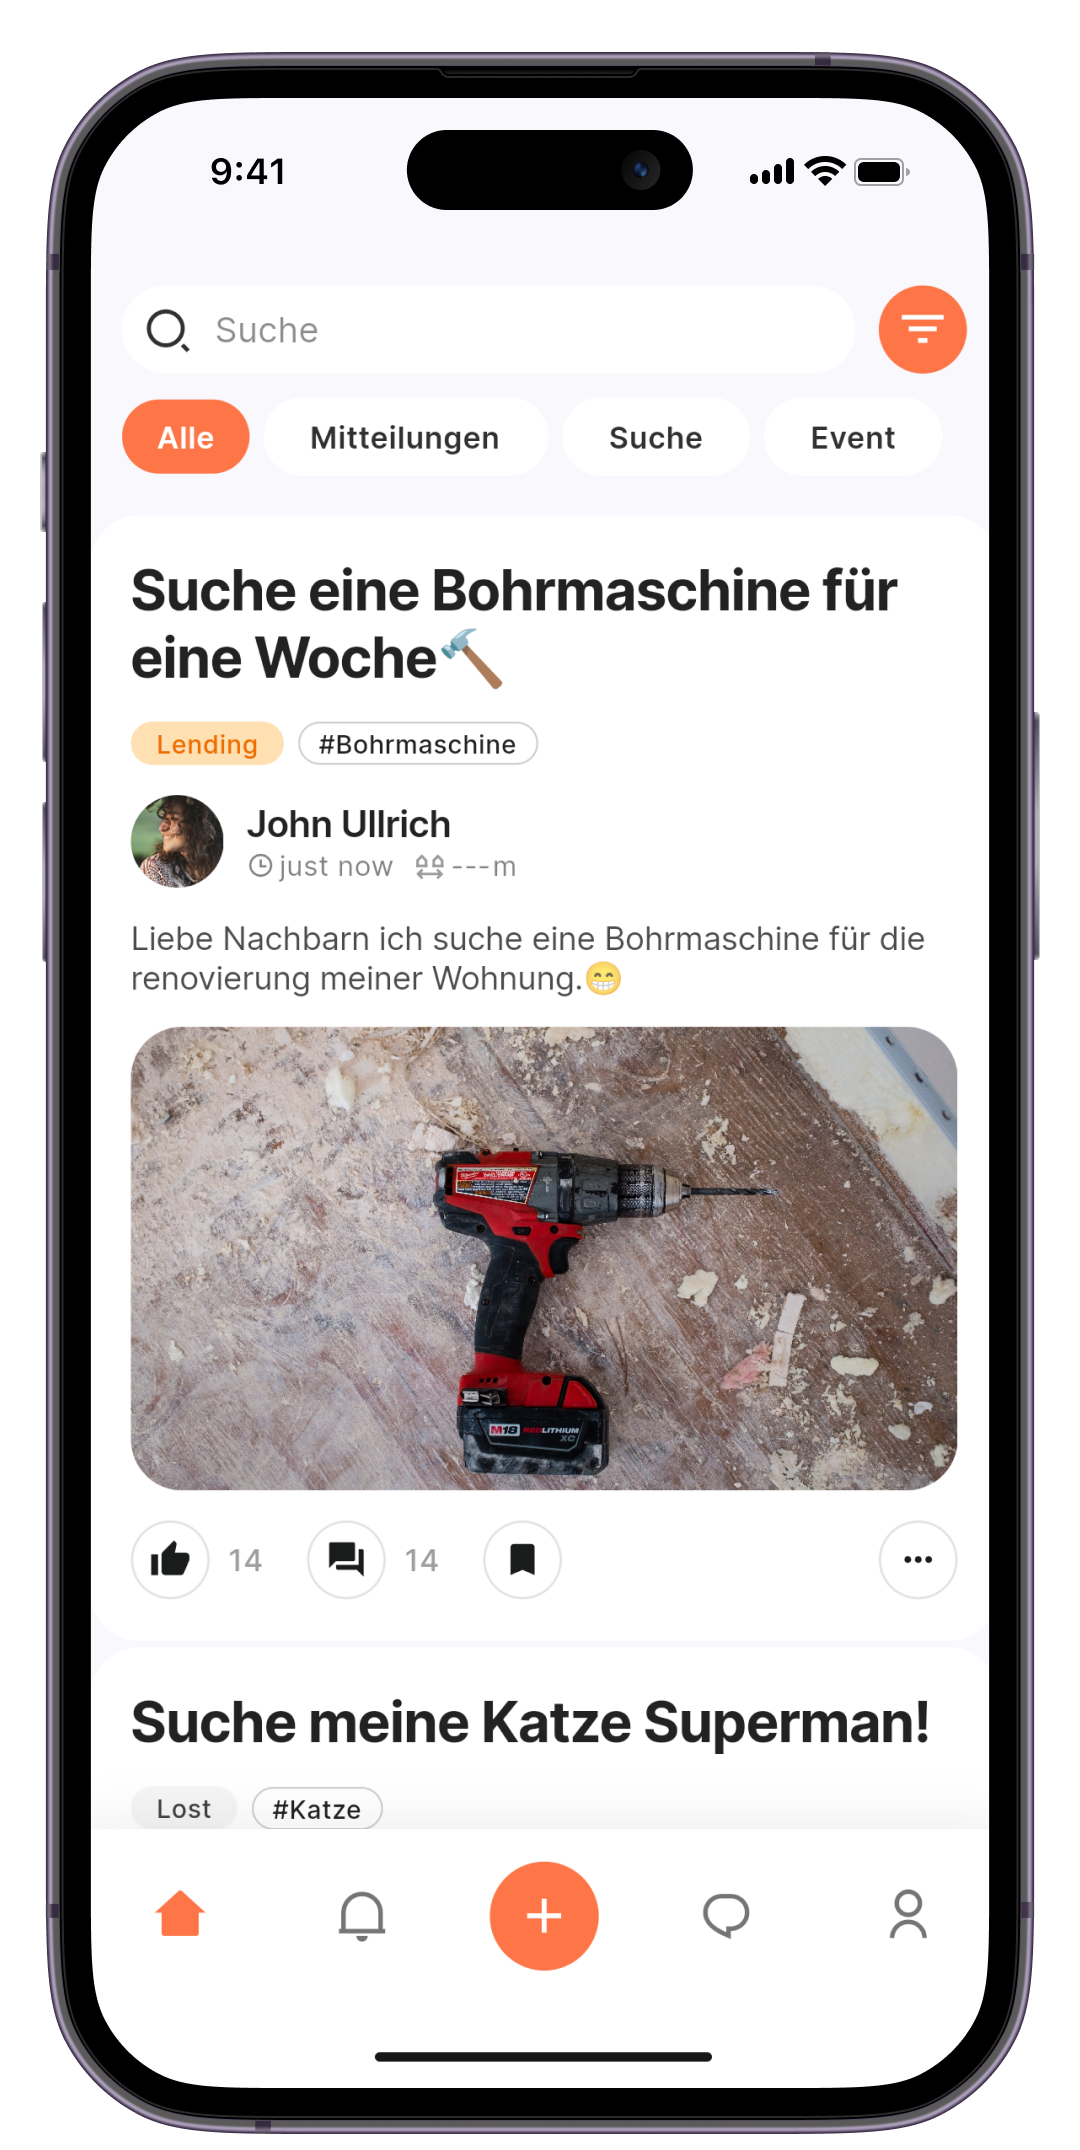
\includegraphics[width=0.3\textwidth]{pics/iphone.png}
  \end{center}
\end{wrapfigure}
The 2018 United Nations study \cite{un2018world} shows that the world population will increase to 9.7 billion people by 2050, with the majority of this increase taking place in urban areas. About 68\% of the world's population is expected to live in cities by 2050. These developments have far-reaching implications for the way we live and work together in cities.

The Nochba project works to strengthen communities and neighbourhoods in urban areas through various social networking initiatives and measures to promote social connections and cohesion between neighbours. With the increase in urban population by 2050, Project Nochba will play an important role in ensuring that neighbourhoods and communities in cities remain liveable and social isolation is reduced.

The app includes a translation function that helps overcome language barriers between community members. This allows users to search for and offer various forms of help to neighbours, such as shopping for elderly neighbours, helping with renovation work, fixing a flat tyre, looking for a lost pet or borrowing tools. The app also serves as a platform to warn neighbours of possible burglaries or other dangers. Users can verify their address when registering via location recognition or QR codes, with QR codes for communities being passed from phone to phone or published by the city or housing associations. Users can define the size of their community by setting a radius in which they can request or offer help via postings. Neighbours can then see and respond to these postings, and the app facilitates communication between those seeking help and those offering it.
\newpage
\begin{spacing}{1}
  \chapter*{Zusammenfassung}
\end{spacing}
\begin{wrapfigure}{r}{0.3\textwidth}
  \begin{center}
    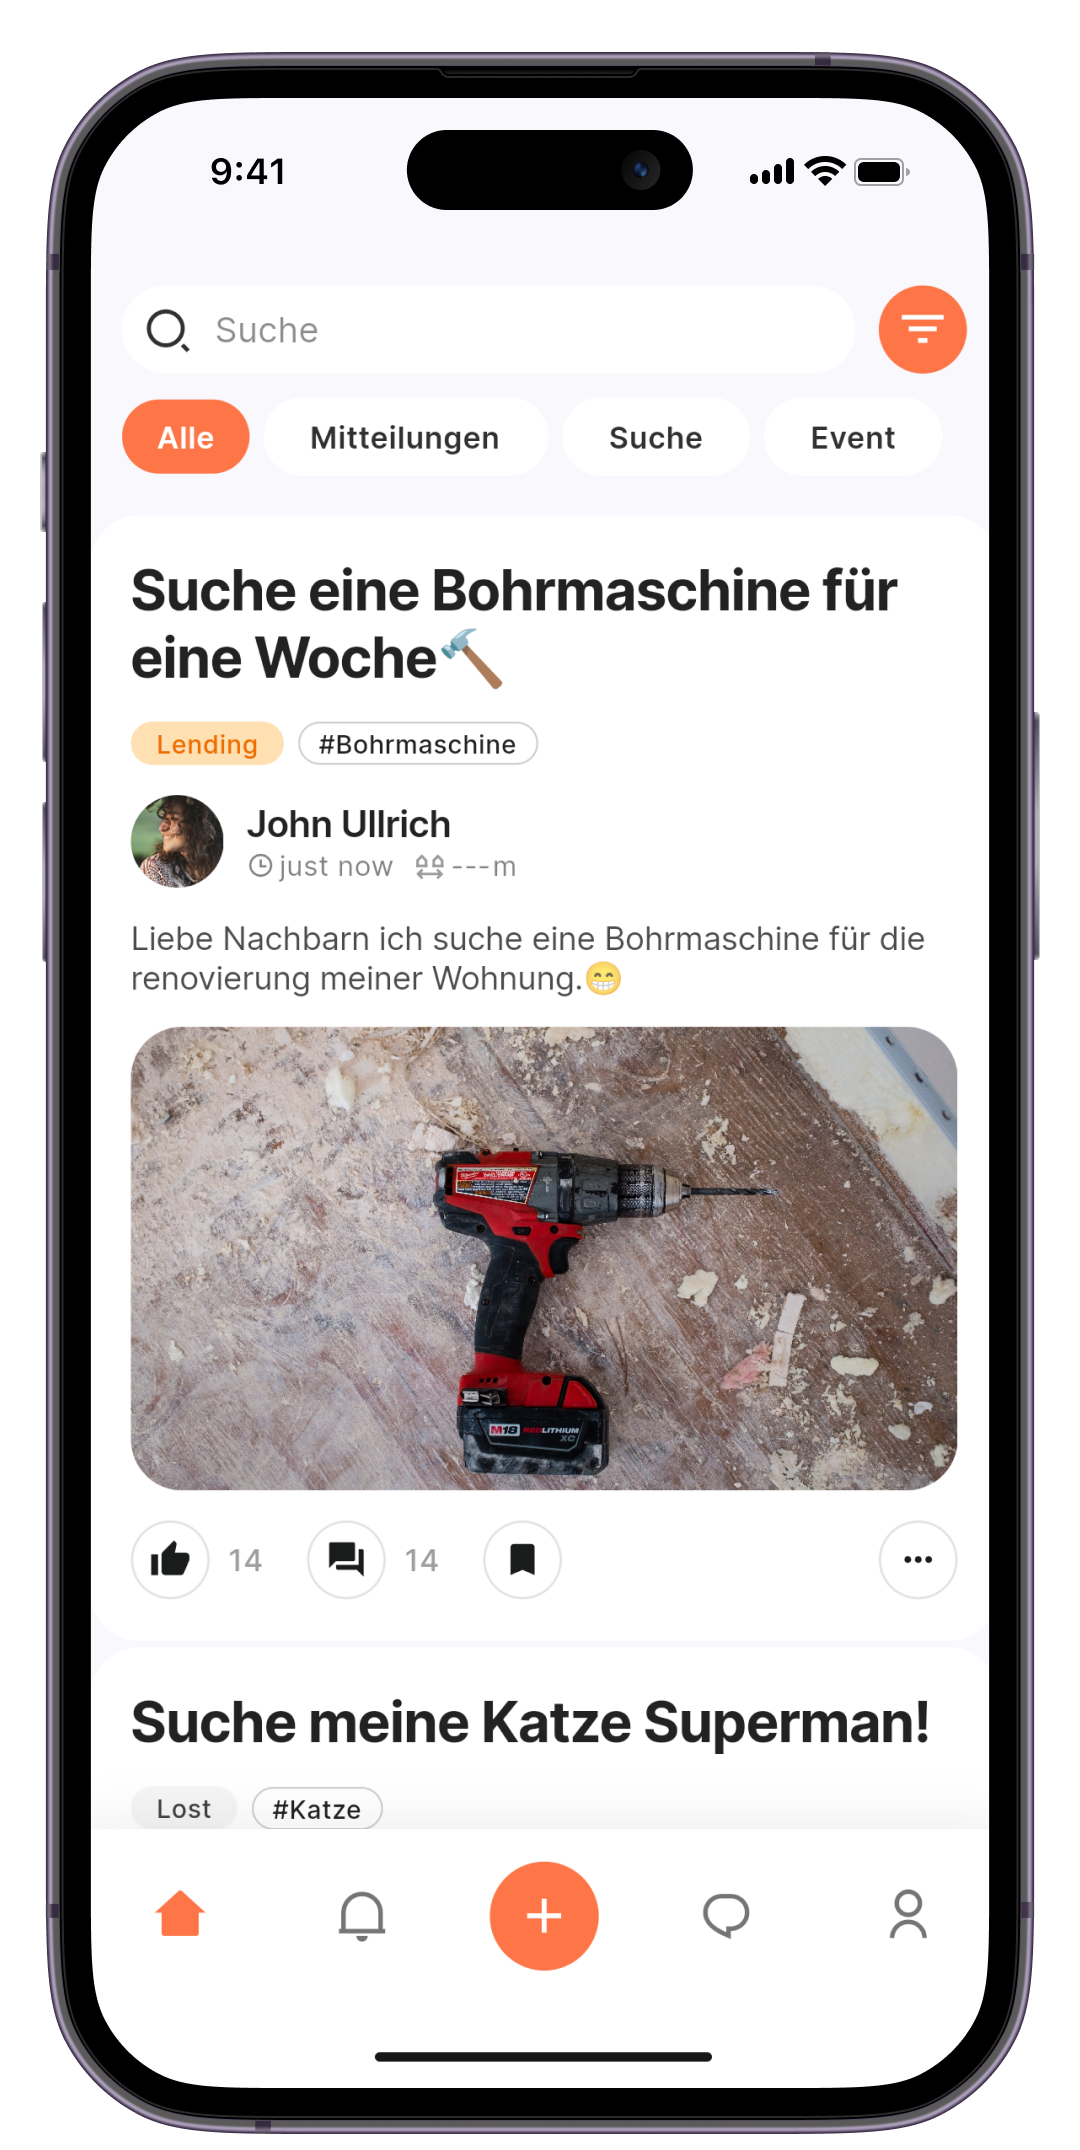
\includegraphics[width=0.3\textwidth]{pics/iphone.png}
  \end{center}
\end{wrapfigure}
Die Studie der Vereinten Nationen \cite{un2018world} aus dem Jahr 2018 zeigt, dass bis 2050 voraussichtlich ein Anstieg der Weltbevölkerung auf 9,7 Milliarden Menschen erwartet wird, wobei der größte Teil dieses Anstiegs in städtischen Gebieten stattfinden wird. Es wird erwartet, dass bis 2050 etwa 68\% der Weltbevölkerung in Städten leben werden. Diese Entwicklungen haben weitreichende Auswirkungen auf die Art und Weise, wie wir in Städten leben und zusammenarbeiten.

Das Projekt Nochba setzt sich dafür ein, die Gemeinschaft und Nachbarschaften in städtischen Gebieten zu stärken, indem es verschiedene Initiativen und Maßnahmen ergreift, um soziale Verbindungen und Zusammenhalt zwischen den Nachbarn zu fördern. Angesichts des Anstiegs der städtischen Bevölkerung bis 2050 wird das Projekt Nochba eine wichtige Rolle dabei spielen, sicherzustellen, dass die Nachbarschaften und Gemeinschaften in Städten weiterhin lebenswert bleiben und dass soziale Isolation reduziert wird.

Die App enthält eine Übersetzungsfunktion, die hilft, Sprachbarrieren zwischen den Mitgliedern der Gemeinschaft zu überwinden. So können die Nutzer unterschiedliche Formen der Nachbarschaftshilfe suchen und anbieten, beispielsweise für ältere Nachbarn einkaufen, bei Renovierungsarbeiten helfen, eine Reifenpanne beheben, ein entlaufenes Haushaustier suchen oder Werkzeuge ausleihen. Die App dient auch als Plattform, um Nachbarn vor möglichen Einbrüchen oder anderen Gefahren zu warnen. Die Nutzer können ihre Adresse während der Registrierung über die Standorterkennung oder QR-Codes verifizieren, wobei QR-Codes für Gemeinschaften von Telefon zu Telefon weitergegeben oder von der Stadt oder Wohnungsbaugenossenschaften veröffentlicht werden. Die Nutzer können die Größe ihrer Community definieren, indem sie einen Radius festlegen, innerhalb dessen sie über Postings Hilfe anfordern oder anbieten können. Die Nachbarn können dann diese Beiträge sehen und darauf antworten, und die App erleichtert die Kommunikation zwischen Hilfesuchenden und Helfern.



\pagestyle{plain}

\renewcommand{\lstlistlistingname}{Quellcodeverzeichnis}

\tableofcontents
\newpage
\setcounter{RPages}{\value{page}}
\setcounter{page}{0}
\pagenumbering{arabic}
\setcounter{secnumdepth}{2}
\setcounter{tocdepth}{2}
\pagestyle{scrheadings}

\begin{spacing}{1}
	\chapter{Einleitung}\label{chapter:introduction}
\end{spacing}
% \lipsum[2-3]

\section{Motivation}
\setauthor{Arsham Edalatkhah}

In der heutigen sich schnell entwickelnden Welt verändert die Urbanisierung die Art und Weise, wie die Menschen leben, rapide, was zu einer zunehmenden Anonymität und Unverbundenheit innerhalb der Nachbarschaft führt. Das Team Nochba hat diese Herausforderung erkannt und eine Möglichkeit gefunden, Gemeinschaften zusammenzubringen und die Verbindung, Zusammenarbeit und Unterstützung zwischen Nachbarn zu fördern.

Durch die Entwicklung einer Social-Media-App, die speziell für die Kommunikation in der Nachbarschaft entwickelt wurde, hofft das Team Nochba, die Kluft zwischen den Gemeindemitgliedern zu überbrücken und ihnen zu helfen, Sprachbarrieren, kulturelle Unterschiede und die Herausforderungen des modernen Stadtlebens zu überwinden. Das Team möchte die Nachbarschaft, wie man sie in den Dörfern kennt, in die Städte bringen.

\section{Aufgabenstellung}
\setauthor{Arsham Edalatkhah}

Das Team Nochba hat es sich auf die Entwicklung einer auf die Nachbarschaft fokussierten Social-Media-App konzentriert, die den Zusammenhalt der Gemeinschaft stärken und den Austausch von Ressourcen unter den Nachbarn erleichtern soll. Das Team hat eine Reihe von Meilensteinen festgelegt, um einen systematischen und effizienten Ablauf des Projekts zu ermöglichen.

Das Team hat sich auf die folgenden Meilensteine geeinigt:

\begin{itemize}
    \item {Entwurf eines Prototypen für die Benutzeroberfläche.}
    \item {Festlegung der Systemarchitektur und Überprüfung der technischen Machbarkeit.}
    \item {Implementierung eines Minimum Viable Product (MVP) mit Funktionen wie Login, Feed, Beitragserstellung, Filter und Chat-Funktion.}
    \item {Ein Minimum Loveable Product (MLP) entwickeln, das Registrierung, Suche, Kontoeinstellungen, Aktivitäten-Tab, Übersetzung, Kommentarfunktion, mehrere Beitragskategorien und ein Reportsystem umfasst.}
    \item {Vervollständigung der Implementierung aller geplanten Funktionen.}
    \item {Beseitigung von Schwachstellen durch Kundenfeedback und Bugfixing.}
    \item {Fertigstellung und Einreichung des Diplomarbeitsprojekts.}
\end{itemize}

Das Team Nochba beabsichtigt, die Arbeit an diesem Projekt auch nach Abschluss der Diplomarbeit fortzusetzen und die App zu verfeinern und zu erweitern, um die Communities besser zu unterstützen und die Verbindung zwischen den Nachbarn zu fördern.

\section{Zusammenfassung des Projektergebnisse}
\setauthor{Arsham Edalatkhah}

\begin{itemize}
    \item \textbf{Auszeichnungen:}
          \begin{itemize}
              \item \textbf{\#1 Platz Linz hACkT Event X Innovationshauptplatz}
              \item \textbf{\#1 Platz mPreneur Austria Contest X ICT4D.at}
              \item \textbf{\#1 Platz Immotopia Innovation Award}
              \item \textbf{\#3 Platz Spusu Innovation Award (Austria - Wien)}
              \item \textbf{Sieger Team bei mPreneur School Ohrid X World Summit Award}
              \item \textbf{Projekt-Präsentation für den Linzer Bürgermeister und Magistrasdirektorin}
              \item \textbf{Veröffentlichung von 'Nochba' im Play Store}
          \end{itemize}
    \item \textbf{Teilnahme an Workshops:}
          \begin{itemize}
              \item \textbf{Workshop Planet Linz Days}
              \item \textbf{Workshop Jugendhackt Österreich}
              \item \textbf{Workshop Project-Forge ICT4D.at}
          \end{itemize}
    \item \textbf{Workshops, die der Arsham Edalatkhah im Rahmen der Diplomarbeit gehostet hat:}
          \begin{itemize}
              \item \textbf{Workshop Präsentationstechnik an der HTL Leonding}
              \item \textbf{Workshop Radio-Training an der HTL Leonding}
          \end{itemize}
    \item \textbf{Medienauftritte:}
          \begin{itemize}
              \item \textbf{Oberösterreicher des Tages (Arsham Edalatkhah)}
              \item \textbf{UNESCO Internet4trust Konferenz}
          \end{itemize}
    \item \textbf{Bevorstehende Events:}
          \begin{itemize}
              \item \textbf{World Summit Award (Austria - Graz)}
              \item \textbf{Project Awards an der HTL Leonding}
          \end{itemize}
\end{itemize}

Seit Beginn des Diplomarbeitsprojekts konzentrierte sich das Team Nochba auf die Entwicklung einer App, die sich auf soziale Aspekte im Bereich des Ressourcen-Sharings und des Community-Buildings konzentriert. Das Ziel des Teams war es, ein Konzept zu entwerfen, das es ermöglicht, auch nach Abschluss der Diplomarbeit einen wertvollen Beitrag für die Gesellschaft zu leisten. Um die IT-Kenntnisse zu vertiefen und von Mentoren und Branchenexperten mehr über das Thema der sozialen Innovation zu erfahren, entschied sich das Team, an einer Reihe von Wettbewerben und Veranstaltungen teilzunehmen.

Durch diese Erfahrungen konnte das Team Nochba eine solide Grundlage für das Projekt schaffen und war davon überzeugt, dass dies ein fundamentaler Bestandteil der Vision sein wird, die das Team zu erfolgreichen Ergebnissen führen wird. Die Kompetenz des Teams im Bereich der nachhaltigen Innovation und sozialen Unternehmerschaft wurde durch die Teilnahme an diesen Wettbewerben unterstrichen. Das Team Nochba freut sich darauf, das Projekt auch nach Abschluss der Diplomarbeit fortzusetzen.

\begin{itemize}
    \item \textbf{Linz-hACkT:}
          \begin{itemize}
              \item \textbf{11. bis 13. März 2022}
          \end{itemize}
\end{itemize}

Während des dreitägigen Linz Hackathon-Events hatte das Team Nochba fünf Mentoren aus verschiedenen Bereichen der IT-Industrie in Österreich und Deutschland, mit denen Coaching-Sessions geplant wurden. Diese Mentoring-Sessions halfen dem Team, die Idee nicht nur aus technischer Sicht zu betrachten, sondern auch aus wirtschaftlicher und sozioökonomischer Perspektive zu analysieren. Sowohl das Team als auch die Mentoren konnten dabei viel lernen. Themen wie Barrierefreiheit und Sicherheit wurden mit erfahrenen Fachleuten aus der Industrie diskutiert, was dem Team einen ersten Überblick über die Vor- und Nachteile des Projekts und die Risiken gab.

Beispielsweise hat das Team gelernt, dass beim Ressourcen-Sharing-Aspekt der Nachbarschaftshilfe-App die ausgetauschten Waren beschädigt zurückgebracht oder sogar gestohlen werden können. Die Wahrscheinlichkeit dafür ist jedoch gering, weil die Nachbarn sich untereinander kennen und daher der bereits bestehende soziale Dynamik eine wichtige Rolle spielt. Der Ruf einer Person hängt auch davon ab, in welchem Zustand die ausgeliehene Ware zurückgebracht wird. Durch die App wird nicht nur die Anzahl der Konflikte innerhalb der Nachbarschaft reduziert, sondern auch der Akt, jemand anderem etwas Gutes zu tun, fördert die Bildung von neuen Freundschaften.

Das Team Nochba hat an dem Wettbewerb Linz hACkT teilgenommen und den ersten Platz erreicht. Dadurch hat das Team die Chance bekommen, gute Beziehungen zur Stadt Linz, zum Innovationshauptplatz Linz und zu Open Common Linz aufzubauen. Am Tag der Preisverleihung erhielt das Team den Linz hACkT-Pokal persönlich von Bürgermeister Klaus Luger.

Seit der Preisverleihung hält das Team des Innovationshauptplatzes ständig über die Fortschritte bei der technischen Weiterentwicklung der Nochba App auf dem Laufenden. Einige Monate später hatte das Team die Chance, am 30. Januar 2023 eine Präsentation für Bürgermeister Klaus Luger und die Magistratsdirektorin Ulrike Huemer zu halten. Das Treffen wurde vom Team des Innovationshauptplatzes organisiert und das Ziel war es, einen Zwischenstandsbericht in Form einer Präsentation über die Leistungen während der Diplomarbeit an der HTL Leonding zu liefern.

\begin{figure}[H]
    \centering
    
\includegraphics[width=1\textwidth]{pics/Linz-hACkT-2022.jpg}
    \caption{Linz hACkT 2022}
    \label{fig:linz-hackt}
\end{figure}


\begin{itemize}
    \item \textbf{ICT4D.at X mPreneur Contest Austria:}
          \begin{itemize}
              \item \textbf{22. September 2022}
          \end{itemize}
\end{itemize}


ICT4D.at ist eine Organisation, die im Jahr 2009 gegründet wurde und sich mit der Förderung und Implementierung von Informations- und Kommunikationstechnologien zur Unterstützung von Menschen in Entwicklungsländern beschäftigt. Die Organisation hat den Fokus auf Innovationen mit den Schwerpunkten Bildung, Gesundheit und Sensibilisierung.

Das Nochba Team entschied sich auf Empfehlung ihrer Betreuungslehrerin, am mPreneur Contest Austria teilzunehmen, um ein Netzwerk auf österreichweites Niveau aufzubauen und die Vision des Projekts Nochba gemeinsam mit den mPreneur-Mentoren zu verfestigen. mPreneur - Social Mobile Entrepreneurship worldwide - ist ein durch Erasmus+ gefördertes Programm.

Schließlich hat das Nochba Team es geschafft, eines der beiden Siegerteams in diesem österreichweiten Wettbewerb zu werden. Als Siegerteam präsentierte das Team das Projekt vor einer internationalen Jury aus Rumänien, Philippinen, Tansania, Uganda, Singapur, Kenia und Österreich. Alle Teammitglieder erhielten für ihre Leistung ein Teilnahmezertifikat von ICT4D und das Nochba Team hat sich dadurch für die Teilnahme an einem interkontinentalen Wettbewerb in Nordmazedonien qualifiziert.

\begin{figure}[H]
    \centering
    \includegraphics[width=1\textwidth]{pics/mPreneur-Austria.JPG}
    \caption{ICT4D.at X mPreneur Contest Austria 2022}
    \label{fig:mpreneur}
\end{figure}

\begin{itemize}
    \item \textbf{Planet Linz Days:}
          \begin{itemize}
              \item \textbf{20. bis 23. Oktober 2022}
          \end{itemize}
\end{itemize}

Der Planet Linz Day ist eine 3-tägige Veranstaltung mit mehreren Workshops, die von den Gewinnern des Linz Hackathon 2022 gehostet werden. Ziel ist es, der Öffentlichkeit die Konzepte nahezubringen, die die Stadtgesellschaft in Linz beeinflussen werden.

Aufgrund des Erfolges bei der Linz hACkT-Veranstaltung wurde das Nochba-Team eingeladen, am Workshop des Planet Linz Days teilzunehmen. Das Team nutzte diese einmalige Gelegenheit, um eine Umfrage in der Stadt Linz durchzuführen, um herauszufinden, wie sich die BewohnerInnen der Stadt eine Social Media Nachbarschaftshilfe-App vorstellen. Nach der Befragung von insgesamt 50 Personen, um die Perspektive der NutzerInnen zu verstehen
stellte das Team fest, dass die folgenden sozialen Dynamiken am wesentlichsten sind:


\begin{itemize}
    \item \textbf{Mitteilung}
          \begin{itemize}
              \item \textbf{Frage}
              \item \textbf{Appell}
              \item \textbf{Warnung}
              \item \textbf{Empfehlung}
              \item \textbf{Gefunden}
          \end{itemize}
    \item \textbf{Suche}
          \begin{itemize}
              \item \textbf{Hilfe}
              \item \textbf{Verloren}
          \end{itemize}
    \item \textbf{Ausleihen}
    \item \textbf{Event}
\end{itemize}


Diese Ergebnisse bildeten die Grundlage für die Liste der Kategorien, in denen Beiträge erstellt werden können. Das Team Nochba nutzte diese Ergebnisse und implementierte sie direkt in die Funktion zur Erstellung von Beiträgen in der App, um die App speziell auf die Bedürfnisse der aktuellen Bewohner der Stadt abzustimmen und eine benutzerfreundliche Erfahrung zu schaffen.

\begin{itemize}
    \item \textbf{Jugend hackt Österreich 2022:}
          \begin{itemize}
              \item \textbf{28. bis 30. Oktober 2022}
          \end{itemize}
\end{itemize}

Jugend Hackt (Quelle: ) ist eine Veranstaltung, die von der Non-Profit Organisation 'Open Knowledge Austria' organisiert wird. Sie veranstaltet eine Reihe von Hackathons, Events und Workshops. Ziel ist es, Innovation und kreative Teamarbeit unter Jugendlichen im Alter von 12 bis 18 Jahren zu fördern.

Das Team Nochba hat sich für die Teilnahme am Wettbewerb Jugend hackt Österreich 2022 entschieden, weil das Modell der Nochba-App perfekt in das Schema der Veranstaltung passt. Jedes Projekt bekommt die Möglichkeit, seine Projektideen vor den Organisatoren der Veranstaltung zu pitchen. Der Wettbewerb wird aufgezeichnet und kann auf der offiziellen 'Dorf TV'-Website und dem offiziellen YouTube-Kanal von Youth Hacks angesehen werden. (Quelle: )


\begin{figure}[H]
    \centering
    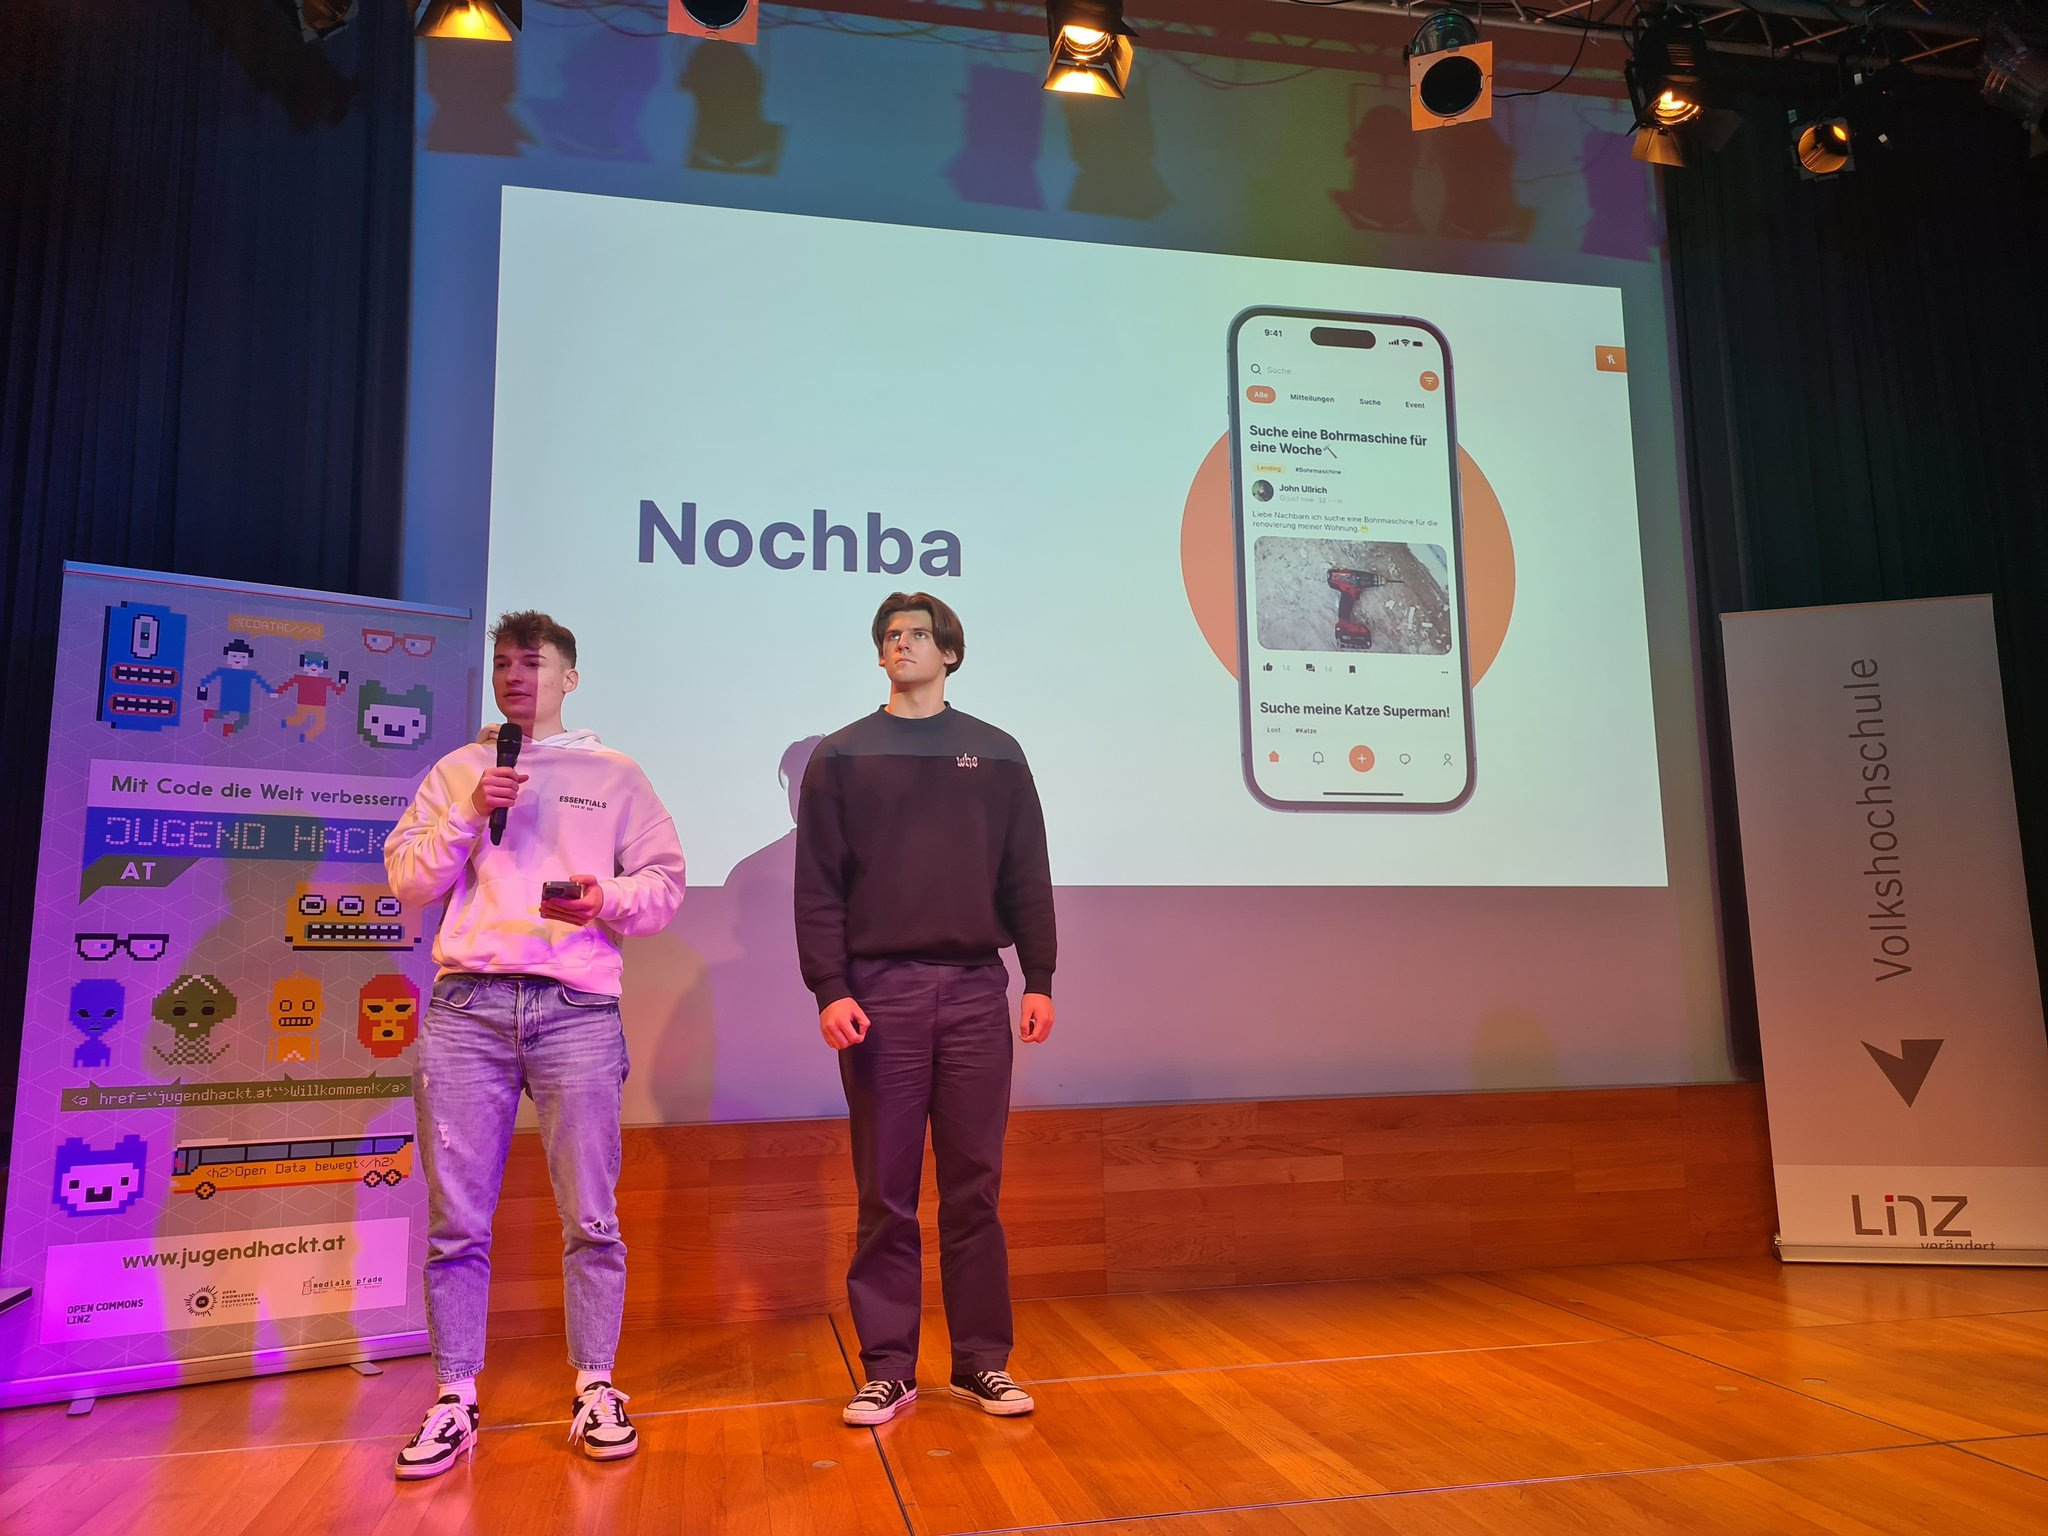
\includegraphics[width=1\textwidth]{pics/JugendHackt.jpeg}
    \caption{Jugend hackt Österreich 2022}
    \label{fig:jugendHackt}
\end{figure}

\begin{itemize}
    \item \textbf{mPreneur School (Ohrid, Nord Mazedonien) X WSA:}
          \begin{itemize}
              \item \textbf{04. bis 09. November 2022}
          \end{itemize}
\end{itemize}

Während der Woche, in der Arsham Edalatkhah an der mPreneur School in Ohrid teilnahm, wurde er mit dem fortgeschrittenen mPreneur School Programm in Form einer non-formalen Ausbildung betreut. Zusammen mit den 16 anderen Teilnehmern aus Asien, Afrika und Europa wurde er von Experten aus verschiedenen Bereichen der Industrie unterrichtet. Die Inhalte der 4 Workshops und der 7 interaktiven Sessions waren Nachhaltiges Entrepreneurship, E-Ethik und soziales Bewusstsein, Künstliche Intelligenz, Big Data und Open Data sowie Virtual Reality / Augmented Reality.

\begin{figure}[H]
    \centering
    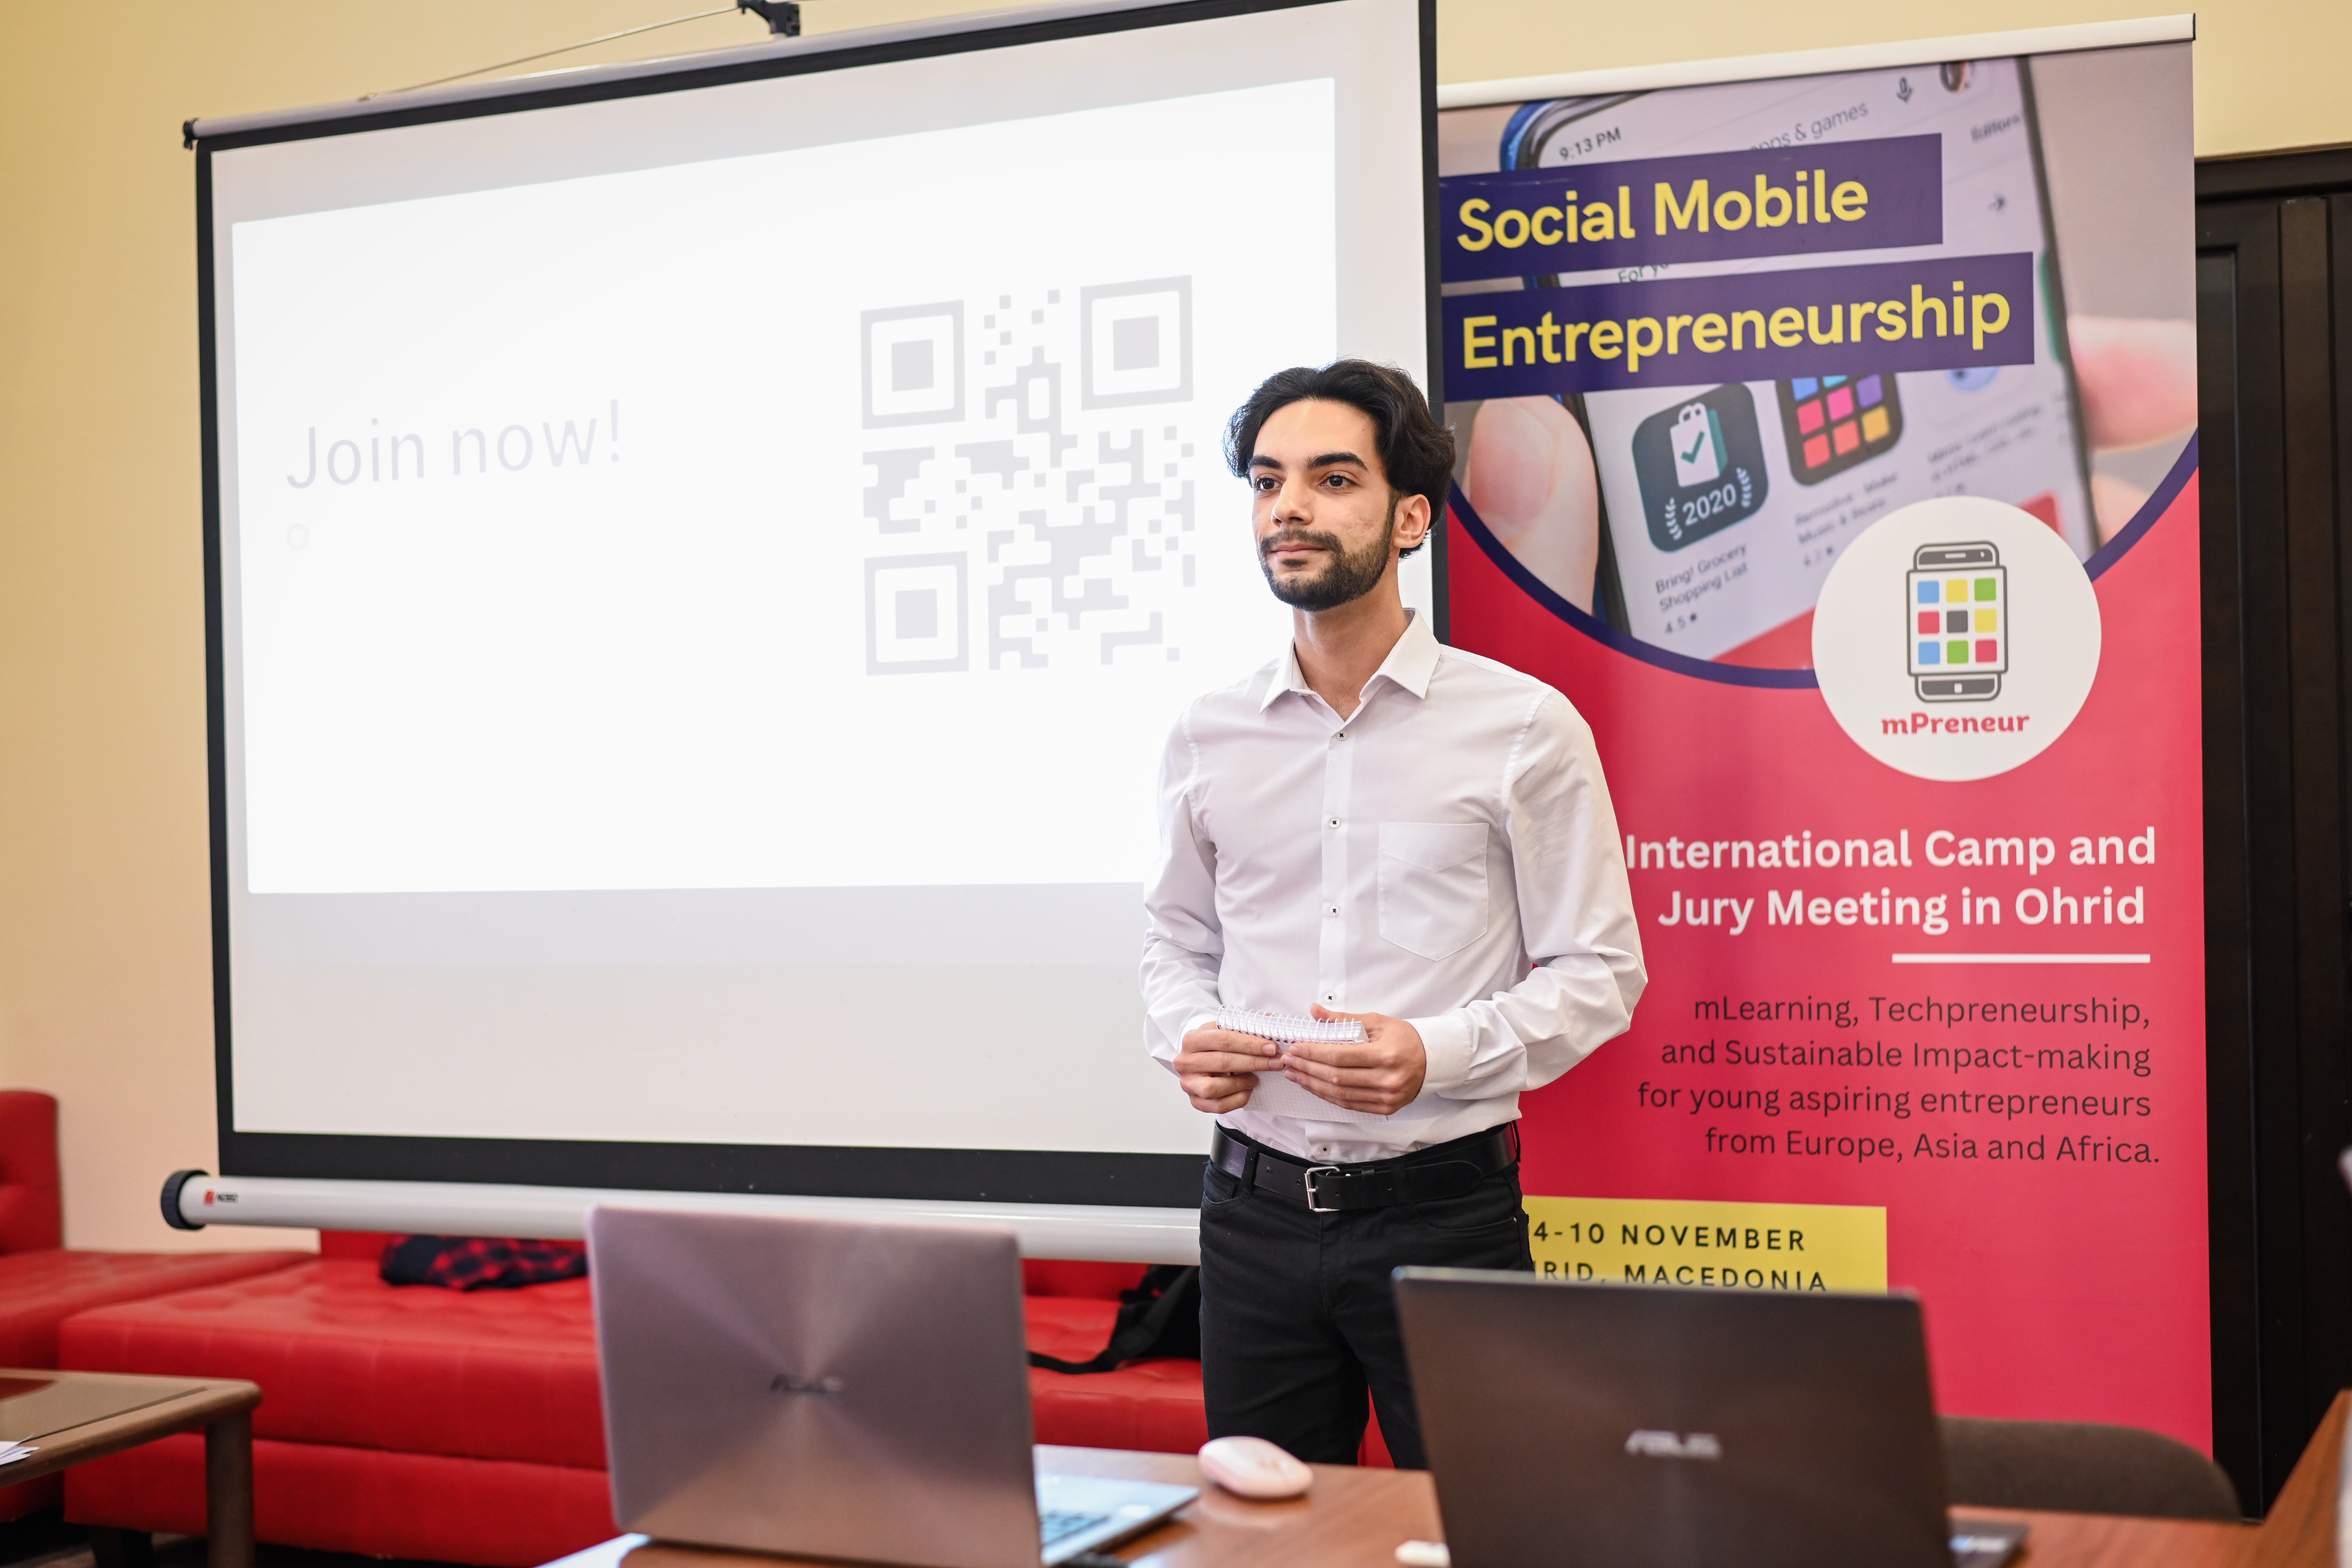
\includegraphics[width=1\textwidth]{pics/mPreneur-2022.JPG}
    \caption{mPreneur School (Ohrid, Nord Mazedonien) X WSA 2022}
    \label{fig:jugendHackt}
\end{figure}

WSA (World Summit Award) ist eine Initiative, die im Jahr 2003 von der österreichischen Regierung gegründet wurde. Ziel ist es, mit die Förderung von nachhaltigen digitalen Produkten einen Beitrag zur Erfüllung der 17 UN SDGs (Sustainable Development Goals - United Nations) zu leisten. Die 17 Ziele für nachhaltige Entwicklung sollen bis zum Jahr 2030 erreicht werden.

\begin{figure}[H]
    \centering
    
\includegraphics[width=1\textwidth]{pics/SDG-17goals.png}
    \caption{17 Sustainable Development Goals - United Nations}
    \label{fig:SDG17goals}
\end{figure}

\begin{enumerate}
    \item \textbf{Keine Armut} - Beseitigung der extremen Armut und Förderung des Wohlstands für alle.
    \item \textbf{Kein Hunger} - Sicherstellung von Ernährungssicherheit und Förderung einer nachhaltigen Landwirtschaft.
    \item \textbf{Gesundheit und Wohlbefinden} - Förderung von Gesundheit und Wohlbefinden für alle Menschen.
    \item \textbf{Hochwertige Bildung} - Zugang zu hochwertiger Bildung für alle, um Wissen und Fähigkeiten zu fördern.
    \item \textbf{Geschlechtergleichheit} - Beseitigung von Diskriminierung aufgrund des Geschlechts und Förderung von Geschlechtergleichheit.
    \item \textbf{Sauberes Wasser und Sanitärversorgung} - Sicherstellung von Zugang zu sauberem Wasser und Sanitärversorgung für alle.
    \item \textbf{Bezahlbare und saubere Energie} - Förderung der Nutzung erneuerbarer Energiequellen und Zugang zu erschwinglicher Energie.
    \item \textbf{Menschenwürdige Arbeit und Wirtschaftswachstum} - Förderung von menschenwürdiger Arbeit und wirtschaftlichem Wachstum.
    \item \textbf{Industrie, Innovation und Infrastruktur} - Förderung von nachhaltiger Industrie, Innovation und Infrastruktur.
    \item \textbf{Weniger Ungleichheit} - Verringerung von Ungleichheit innerhalb und zwischen Ländern.
    \item \textbf{Nachhaltige Städte und Gemeinden} - Förderung von nachhaltigen Städten und Gemeinden durch z. B. effiziente Verkehrs- und Abfallwirtschaft.
    \item \textbf{Nachhaltige/r Konsum und Produktion} - Förderung von nachhaltigem Konsum und Produktion durch z. B. Recycling und Ressourceneffizienz.
    \item \textbf{Maßnahmen zum Klimaschutz} - Bekämpfung des Klimawandels durch Reduzierung von Treibhausgasemissionen und Anpassung an dessen Folgen.
    \item \textbf{Leben unter Wasser} - Schutz der Ozeane, Meere und maritimen Ressourcen für eine nachhaltige Nutzung.
    \item \textbf{Leben an Land} - Schutz der Ökosysteme an Land und Erhaltung der biologischen Vielfalt.
    \item \textbf{Frieden, Gerechtigkeit und starke Institutionen} - Förderung von Frieden, Gerechtigkeit und starken Institutionen für nachhaltige Entwicklung.
    \item \textbf{Partnerschaften zur Erreichung der Ziele} - Aufbau von Partnerschaften zwischen Regierungen, Privatwirtschaft und Zivilgesellschaft zur Erreichung der SDGs.
\end{enumerate}


Alle Länder der Vereinten Nationen haben sich auf diese Agenda für die Zukunft geeinigt. Projekt Nochba ist laut der offiziellen mPreneur Webseite (Quelle \cite{mPreneur-Website}) in 5 der 17 Sustainable Development Goals kategorisiert.

Hier sind die 5 Kategorien:

\begin{itemize}
    \item \textbf{Nachhaltiges Entwicklungsziel Nummer 3:}
          \begin{itemize}
              \item \textbf{Gute Gesundheit und Wohlbefinden}
          \end{itemize}
\end{itemize}

SDG Nummer 3 ist das wichtigste Ziel, und Projekt Nochba ist nun offiziell eines der Projekte, die helfen, Ziel Nummer drei zu erreichen, nämlich Gesundheit und Wohlbefinden für alle Menschen, unabhängig von ihrem Alter.

Studien der Forscher der Brigham Young University zum Thema 'Loneliness and Social Isolation as Risk Factors for Mortality: A Meta-Analytic Review' (Quelle \cite{Loneliness-and-Social-Isolation}) zeigen, dass das Gefühl der Einsamkeit dem Rauchen von 15 Zigarren pro Tag entspricht.Die Nochba App trägt zu diesem Ziel bei, indem sie eine sichere virtuelle soziale Dynamik innerhalb einer lokalen Gemeinschaft schafft, in der Menschen unabhängig von ihrem kulturellen Hintergrund und der Sprachbarriere Verbindungen aufbauen oder sogar neue Freundschaften schließen können. So wird Projekt Nochba mit der Social-Media-App für die Nachbarschaft genau dieses Problem der Gesundheit und Einsamkeit aufgreifen.

\begin{figure}[H]
    \centering
    
\includegraphics[width=0.3\textwidth]{pics/3-Gesundheit-und-Wohlbefinden.png}
    \caption{Nachhaltiges Entwicklungsziel Nr. 3: Gute Gesundheit und Wohlbefinden}
    \label{fig:SDG03}
\end{figure}

\begin{itemize}
    \item \textbf{Nachhaltiges Entwicklungsziel Nr. 4:}
          \begin{itemize}
              \item \textbf{Qualitativ hochwertige Bildung}
          \end{itemize}
\end{itemize}

Ziel des SDG Nummer 4 ist es, bis 2030 die Bildungsmöglichkeiten für alle Menschen, unabhängig von ihrem Alter, zu sichern. Vor allem in den Entwicklungsländern, wo es schwierig sein kann, eine qualitativ hochwertige Bildung zu gewährleisten. Ein Aspekt der Qualität der Bildung ist der Zugang zu Nachhilfelehrern.

Die Nochba App trägt zu dieser Herausforderung bei, da sie über eine innovative Funktion verfügt, mit der jeder Nutzer seinen eigenen individuellen Radius festlegen kann, innerhalb dessen er sich mit seinen Nachbarn verbinden kann. Diese Funktion ermöglicht es den Nutzern, nach Menschen mit den gleichen Interessen wie sie zu suchen und lokale Veranstaltungen zu organisieren. Unter Umständen können Lerngruppen gebildet werden, zu denen jeder Lehrer in der Nähe beitragen kann, was eine sinnvolle Hilfestellung für Studenten und Schüler sein wird, die in der Nachbarschaft pädagogische Unterstützung benötigen.

\begin{figure}[H]
    \centering
    
\includegraphics[width=0.3\textwidth]{pics/SDG-04.jpg}
    \caption{Nachhaltiges Entwicklungsziel Nr. 4: Qualitativ hochwertige Bildung}
    \label{fig:SDG04}
\end{figure}

\begin{itemize}
    \item \textbf{Nachhaltiges Entwicklungsziel Nr. 11:}
          \begin{itemize}
              \item \textbf{Nachhaltige Städte und Gemeinden}
          \end{itemize}
\end{itemize}

Nachhaltigkeit in den Städten und Gemeinden spielt in der Agenda 2030 eine wichtige Rolle. Ziel ist es, leistbare Häuser und Wohnungen zu schaffen und gleichzeitig dafür zu sorgen, dass die Lebensbedingungen sicher sind. Einerseits geht es darum, Ordnung in die Slums zu bringen, andererseits soll sichergestellt werden, dass die Menschen in den verschiedenen Gemeinden Zugang zu sicheren öffentlichen Verkehrssystemen haben. Ziel ist es, die Umweltverschmutzung zu verringern, indem der Öffentlichkeit Zugang zu öffentlichen Verkehrssystemen verschafft wird.

Die Menschen, die am meisten von solchen Bewegungen innerhalb der Gemeinden und Stadtteile profitieren, sind die Bedürftigen. SDG Nummer 11 hat direkte Auswirkungen auf das Leben der Armen und Benachteiligten. Die Verwirklichung dieses Ziels wird die Lebensbedingungen von Frauen, Kindern und älteren Menschen sicherer machen. Insgesamt wird der Wandel in die richtige Richtung letztendlich gesündere Gemeinschaften schaffen und zur finanziellen, sozioökonomischen und ökologischen Stärkung der Gemeinschaften in städtischen und ländlichen Gebieten beitragen.

Die Studien des United Nations Department of Economics and Social Affairs (UN DESA) 2018 'Revision of World Urbanization Prospects report' \cite{Worlds-Urbanization-Prospects} zeigen, dass 70\% der Bevölkerung in den Städten leben werden und dass es drei Quellen für das Bevölkerungswachstum gibt:

\begin{enumerate}
    \item \textbf{Das natürliche Wachstum der Bevölkerung innerhalb der städtischen Gebiete}
    \item \textbf{Migration (insbesondere in Ländern, in denen die Zuwanderung die Abwanderung übersteigt)}
    \item \textbf{Umgliederungen von ländlichen in städtische Gebiete}
\end{enumerate}

Die Vision der Nochba App ist es, einen starken Einfluss auf die sozioökonomische Seite des alltäglichen Lebens in städtischen Gemeinden zu haben. Diese Studie über 'die Beziehung zwischen Charakteristika der Nachbarschaft und Einsamkeit bei älteren Erwachsenen in Amsterdam, Niederlande: Eine bevölkerungsbasierte Studie' \cite{neighbourhood-characteristics-and-loneliness} zeigt, dass das Gefühl, nur eine Nummer zu sein, in Großstädten mit vielen Einwohnern häufiger auftritt als in Gemeinden in ländlichen Gebieten.

Die Nochba App bringt das Konzept der Nachbarschaft, wie es in ländlichen Gebieten bekannt ist, in die Stadtviertel, um das Gefühl der Einsamkeit und Isolation in größeren Gemeinschaften zu bekämpfen und stattdessen die Nachbarschaft zu stärken, indem sie die gemeinsame Nutzung von Ressourcen und die Bildung von Gemeinschaften unter den Stadtbewohnern fördert.

\begin{figure}[H]
    \centering
    
\includegraphics[width=0.3\textwidth]{pics/sdg-image-11-data.png}
    \caption{Nachhaltiges Entwicklungsziel Nr. 11: Nachhaltige Städte und Gemeinden}
    \label{fig:SDG11}
\end{figure}

\begin{itemize}
    \item \textbf{Nachhaltiges Entwicklungsziel Nr. 12:}
          \begin{itemize}
              \item \textbf{Verantwortungsbewusster Konsum und Produktion}
          \end{itemize}
\end{itemize}

Ziel Nr. 12 der SGD ist es, die Nahrungsmittelverschwendung pro Person weltweit auf die Hälfte zu reduzieren. Im Rahmen dieses zehnjährigen Programms ergreifen alle weiter industrialisierten Länder Maßnahmen, um zu einem nachhaltigen Konsum und einer nachhaltigen Produktion voranzuschreiten. Die Menge der verwendeten fossilen Brennstoffe hat ebenfalls einen Einfluss auf die Erreichung des Ziels der Umweltverträglichkeit, insbesondere die ineffiziente Nutzung der Brennstoffe.

Die Strategie besteht darin, nachhaltige Methoden im öffentlichen Produktionssektor zu fördern und all dies in Übereinstimmung mit den lokalen Bedürfnissen und den nationalen Regierungspolitiken und -prioritäten zu betreiben. Außerdem soll sichergestellt werden, dass die Informationen verbreitet werden, so dass das Bewusstsein in der Bevölkerung steigt, während die Maßnahmen getroffen werden, um zu gewährleisten, dass nicht nur die Produzenten, sondern auch die Verbraucher dazu beitragen. Schließlich soll dieses wichtige Ziel bis 2030 erreicht werden, um eine gesunde Umwelt für alle zu schaffen.

Nach den Studien der Ernährungs- und Landwirtschaftsorganisation der Vereinten Nationen (FAO) (Quelle: \cite{bcg2018foodloss} ) über die weltweite Nahrungsmittelverschwendung pro Kopf der Bevölkerung werden jedes Jahr etwa 1,6 Milliarden Tonnen Lebensmittel verschwendet. Das ist ein Drittel aller Lebensmittel, die jedes Jahr für die Verbraucher produziert und hergestellt werden. Demselben Bericht zufolge beträgt die durchschnittliche Menge an verschwendeten Lebensmitteln pro Kopf etwa 120 kg pro Jahr. In den Industrieländern ist diese Menge noch viel höher und erreicht einen Spitzenwert von fast 300 kg pro Jahr. Am unteren Ende der Skala, vor allem in den Entwicklungsländern, ist diese Zahl erstaunlich niedrig und die Menge an verschwendeten Lebensmitteln pro Kopf liegt bei 6 bis 11 kg pro Jahr.

Eine weitere Studie der Boston Consulting Group (BCG) (Quelle: \cite{bcg2022foodwaste} ) zeigt, welche Kosten diese Menge an Lebensmittelabfällen verursacht und welche Auswirkungen sie auf die Weltwirtschaft hat. Laut dieser Studie kostet die Lebensmittelverschwendung jedes Jahr schätzungsweise 1,5 Billionen Dollar. Dieselbe Studie hat auch herausgefunden, dass die Reduzierung der Lebensmittelabfälle zu positiven Ergebnissen in allen wichtigen Aspekten der Industrie führen kann. Die Reduzierung der Lebensmittelabfälle könnte einen erheblichen und bemerkenswerten wirtschaftlichen, sozialen und eviromentalen Nutzen bringen. Dazu gehört auch die Schaffung von neuen Arbeitsplätzen. Dadurch wird die Menge an Treibhausgasen, die pro Jahr erzeugt wird, reduziert und die Ernährungssicherheit erhöht.

Die Nochba App trägt zu SGD Nummer 12 bei, da sie einen Service bietet, bei dem Ressourcen im Allgemeinen geteilt und somit effizienter genutzt werden. Insbesondere das Teilen von Lebensmitteln spielt eine große Rolle, wenn es um die Sharing Economy in städtischen Gemeinschaften geht.

Im Laufe der Jahre wurden mehrere Studien durchgeführt, die belegen, dass die Menge der pro Kopf und Jahr verschwendeten Lebensmittel sinkt, sobald es ein Foodsharing-Netzwerk gibt. (Quelle: \cite{parizeau2015food} ) Forscher fanden auch heraus, dass besonders in städtischen Gemeinden die Lebensmittelverschwendung abnimmt und gleichzeitig das soziale Netzwerk und der Gemeinschaftssinn und damit der soziale Zusammenhalt in den Städten zunimmt.  Die Nochba App ist ein weiterer Schritt in diese Richtung, da sie die Lebensmittelverschwendung in städtischen Gemeinden weiter reduziert und gleichzeitig die soziale Interaktion und den Zusammenhalt in den Gemeinden fördert.


\begin{figure}[H]
    \centering
    
\includegraphics[width=0.3\textwidth]{pics/SDG-12.png}
    \caption{Nachhaltiges Entwicklungsziel Nr. 12: Verantwortungsbewusster Konsum und Produktion}
    \label{fig:SDG12}
\end{figure}

\begin{itemize}
    \item \textbf{Nachhaltiges Entwicklungsziel Nr. 16: }
          \begin{itemize}
              \item \textbf{Frieden, Gerechtigkeit und starke Institutionen}
          \end{itemize}
\end{itemize}

Das Ziel Nr. 16 für nachhaltige Entwicklung zielt auf Gewalt und Diskriminierung ab. Es geht um die Stärkung der Institutionen auf allen Ebenen. Durch den Aufbau wirksamer und starker Institutionen auf lokaler, nationaler und internationaler Ebene. Diese Institutionen müssen transparent und rechenschaftspflichtig sein und auf die Bedürfnisse aller Menschen eingehen. Mit dem Schwerpunkt auf Frieden, Gerechtigkeit und starken Institutionen als entscheidende Grundlagen für eine nachhaltige Entwicklung bis 2030. Die Bekämpfung von Korruption und Bestechung beinhaltet die Entwicklung rechenschaftspflichtiger und wirksamer Institutionen auf allen Ebenen. In diesem Fall ist es wichtig, die Meinung der Bevölkerung zu berücksichtigen, indem Umfragen und Workshops unter Einbeziehung der Öffentlichkeit durchgeführt werden.

Eine im Jahr 2021 veröffentlichte Studie mit dem Titel 'The impact of COVID-19 on social isolation among older immigrants in Canada: language barriers and access to information' (Quelle: ) zeigt einige interessante Ergebnisse darüber, wie Sprachbarrieren und kulturelle Unterschiede zur Bildung isolierter Gruppen führen können und wie sich die COVID-19-Pandemie auf dieses Problem ausgewirkt hat. Durch eine Reihe von Interviews mit einer Gruppe älterer Einwanderer, die in Kanada leben und mit Sprachbarrieren und kulturellen Unterschieden konfrontiert sind, fanden sie heraus, dass sie die soziale Isolation auf einem höheren Niveau erlebten und dass die soziale Isolation während der COVID-19-Pandemie noch intensiver wurde, weil der Zugang zu sozialen Interaktionen und damit auch der Zugang zu entsprechenden Informationen eingeschränkt war.

Nach der gleichen Studie gibt es 5 Motivatoren für Teilnehmer, die sich einer Gemeinschaft anschließen wollen. Diese Motivatoren sind:

\begin{enumerate}
    \item \textbf{Emotionen und Moral}
    \item \textbf{Identität und Gefühl der Gemeinschaft}
    \item \textbf{Belohnung}
    \item \textbf{Sozialer Einfluss}
    \item \textbf{Instrumentalität}
\end{enumerate}

Instrumentalität beschreibt im Wesentlichen Ziele mit einer starken motivierenden Wirkung, wie z. B. die Rettung von Lebensmitteln vor der Verschwendung und die Verbreitung eines neuen Bewusstseins und einer neuen Mentalität gegenüber dem Nahrungsmittelverbrauch.

Die Nochba-App trägt zu diesem Ziel bei, indem sie das erforderliche Netzwerk innerhalb der Nachbarschaftsgemeinschaften schafft, um Ressourcen gemeinsam zu nutzen. Auf diese Weise wird die Nochba-App die Lebensmittelverschwendung in städtischen Gemeinden weiter reduzieren und gleichzeitig die soziale Interaktion und den Zusammenhalt der Gemeinschaft fördern.

\begin{figure}[H]
    \centering
    
\includegraphics[width=0.3\textwidth]{pics/SDG-16.png}
    \caption{Nachhaltiges Entwicklungsziel Nr. 16: Frieden, Gerechtigkeit und starke Institutionen}
    \label{fig:SDG16}
\end{figure}

\begin{itemize}
    \item \textbf{Immotopia Innovation Award:}
          \begin{itemize}
              \item \textbf{15. Februar 2023}
          \end{itemize}
\end{itemize}

Der Immotopia Innovation Award ist ein Wettbewerb, der von der Regionalzeitung Oberösterreich Nachrichten und Compact Projektentwicklungs GmbH organisiert wird, um Projekte zu prämieren, die in den folgenden Kategorien einen besonderen Einfluss haben:

\begin{itemize}
    \item \textbf{Nachhaltigkeit:}
          \begin{itemize}
              \item \textbf{Umweltfreundliche Baupraktiken oder die Entwicklung von nachhaltigen Gemeinschaften.}
          \end{itemize}
    \item \textbf{Innovation:}
          \begin{itemize}
              \item \textbf{Neue und innovative Ansätze bei der Planung und dem Bau von Gebäuden}
          \end{itemize}
    \item \textbf{Soziale Verantwortung:}
          \begin{itemize}
              \item \textbf{Positive Einflussnahme auf lokale Gemeinschaften oder soziale Problemstellungen}
          \end{itemize}
    \item \textbf{Digitalisierung:}
          \begin{itemize}
              \item \textbf{Verbesserung der Effizienz, Sicherheit oder Nachhaltigkeit von Gemeinschaften in ländlichen und städtischen Gebieten}
          \end{itemize}
    \item \textbf{Integration:}
          \begin{itemize}
              \item \textbf{Integration und Inklusivität, Schaffung von leistbarem Wohnraum und Integration von marginalisierten Gruppen.}
          \end{itemize}
\end{itemize}

Die Nocha-App schaffte es in der Kategorie Digitale Unterstützung auf den ersten Platz und wurde daher vom Wettbewerbssponsor HYPO Oberösterreich und OÖNachrichten mit 2000 € gefördert.

\begin{figure}[H]
    \centering
    
\includegraphics[width=1\textwidth]{pics/Immotopia-2023.jpg}
    \caption{Immotopia Innovation Award 2023}
    \label{fig:Immotopia2023}
\end{figure}

\begin{itemize}
    \item \textbf{Workshop Präsentationstechnik (HTL Leonding):}
          \begin{itemize}
              \item \textbf{16. Februar 2023}
          \end{itemize}
\end{itemize}


Für den Pitch am Ende des mPreneur Social Mobile Entrpreneurship in Ohrid nahm Arsham Edalatkhah an etwa 6 bis 8 Online-Trainingseinheiten zur Vorbereitung mit drei Jurymitgliedern des World Summit Award teil. Er lernte viel über die Kunst des Pitchings und beschloss daher, eines der WSA-Jurymitglieder einzuladen, einen 120-minütigen Workshop über Präsentationstechniken zu halten. Der Präsentationstechnik-Workshop wurde von Arsham Edalatkhah organisiert, um den Horizont der SchülerInnen der HTL Leonding zu erweitern und ihnen zu helfen, qualitativ hochwertige Präsentationen in verschiedenen Situationen vorzubereiten. Der Inhalt des Workshops besteht aus dem über 10-jährigen Wissen und der Erfahrung des Gastgebers auf dem Gebiet der Präsentation und des Pitchings.

Parallel dazu hat Arsham Edalatkhah innerhalb der HTL Leonding eine ganze Community namens 'The Creative Masterminds Community' mit über 60 Mitgliedern gegründet. Er lud die Mitglieder dieser Community und alle Schülerinnen und Schüler der Abschlussklasse der HTL Leonding ein, an dem Workshop teilzunehmen. Am Ende schaffte er es, den ganzen Seminarraum mit Schülern zu füllen, die interessante Fragen stellten, sich Notizen machten und vor allem etwas Nützliches für ihr Berufsleben und ihre Karriere lernten.

Die folgenden theoretischen Themen wurden während des Workshops ausführlich diskutiert:


\begin{itemize}
    \item {Wie bereitet man sich am besten auf die mündlichen Reifeprüfungen vor?}
    \item {Was ist der Unterschied zwischen einer Projektpräsentation im Unterricht und im Berufsleben? Welche Details sind dabei zu beachten, die den Schülern an der HTL Leonding nicht vermittelt werden?}
    \item {Wie gestaltet man am besten die Themen und die Struktur für die Präsentation?}
    \item {Wie kann man trainieren, um am besten mit der Stimme, der Körpersprache und dem Blickkontakt zu kommunizieren?}
    \item {Was sollte man anziehen?}
    \item {Wie kann man das, was man präsentiert, an das Publikum anpassen?}
    \item {Was sollte man niemals sagen oder tun?}
    \item {Wie kann man seine Folien am besten gestalten?}
    \item {Wie kann man mit Nervosität umgehen?}
\end{itemize}

Zwei Monate vor dem Tag des Workshops lud Arsham Edalatkhah zwei engagierte Schülerinnen ein, ein Live-Beispiel für den Workshop vorzubereiten. Die Vorbereitung erfolgte in 6 Online-Sitzungen mit dem Moderator, den Organisatoren und den Vortragenden selbst. Das Team diskutierte 3 Szenarien für den praktischen Teil. Jeder Referent wählte ein Szenario und übte für den praktischen Teil. Anschließend gab es alle zwei Wochen eine Feedback-Sitzung bis zum Tag des Seminars. Während der Vorbereitungsphase hat das Workshop-Team die folgenden praktischen Beispiele eingeübt, die dazu dienten, dem Publikum den theoretischen Teil des Workshops live zu zeigen:

\begin{itemize}
    \item \textbf{Szenario Nummer eins: }
          \begin{itemize}
              \item {Vorstellung eines Projekts in Form eines Investoren-Pitches für ein Jury-Team:

                    Das für dieses Beispiel verwendete Projekt war eine Abschlussarbeit, die von den Studenten der Abschlussklasse der HTL Leonding entwickelt wurde. 'Schrödingers Haus: Ein Escape Room' Ein Virtual-Reality-Spiel, das den Escape Room in jedes Wohnzimmer bringt. Die Familienmitglieder und Freunde des Spielers können gemeinsam helfen, die Rätsel in der Spielwelt zu lösen. Während der Spieler Spielerfahrung sammelt, können die anderen die Story des aktuellen Levels nachlesen und dem Spieler mit ihren Tipps dabei helfen, sich durch die Spielwelt zu navigieren, um aus dem Raum zu entkommen.}
          \end{itemize}
    \item \textbf{Szenario Nummer zwei: }
          \begin{itemize}
              \item {Einer Gruppe Eltern mit ihren Kindern, die sich für einen Besuch der HTL Leonding interessieren, die Vorteile der Ausbildung an der HTL Leonding beim Tag der offenen Tür erklären.}
          \end{itemize}
\end{itemize}

\begin{itemize}
    \item \textbf{ICT4D.at Project-Forge Workshop 2022 (Wien):}
          \begin{itemize}
              \item \textbf{30. November 2022}
          \end{itemize}
\end{itemize}


Die Project-Forge (Quelle: ) ist ein einzigartig strukturierter Workshop, bei dem mehrere Mitglieder und zusätzliche Gäste zusammenkommen, um eine Reihe von verschiedenen ICT4D.at-Projekten aus unterschiedlichen Regionen der Welt zu diskutieren. Jedes Projekt bekommt zwei Minuten Zeit, um die Idee vorzustellen und alle Anwesenden kurz über das Projekt zu informieren, gefolgt von einer 30-minütigen Diskussionsrunde, in der jedes Projekt mit den Anwesenden, die sich für das jeweilige Projekt interessieren, im Detail analysiert und diskutiert werden. Ziel ist es, die vorliegenden Konzepte zu erweitern und die Visionen der einzelnen Projekte zu schärfen.

Ziel ist es, durch die offene Diskussion der Projekte, den Austausch von Tipps, das Hinterfragen und Kommentieren des Prozesses die Möglichkeit zu schaffen, den bestehenden Ideen einen zusätzlichen Wert zu verleihen und die Visionen der einzelnen Projekte zu schärfen.

Dies sind die Projekte, die diskutiert wurden:

\begin{itemize}
    \item \textbf{Teaching in India}
    \item \textbf{Cooperation with Farm Radio}
    \item \textbf{Free online courses on data management and monitoring for NGOs}
    \item \textbf{University Project Kenya - DigiLab}
\end{itemize}

Aufgrund des Erfolges der Nochba App beim vergangenen ICT4D.at Wettbewerb wurde das Nochba Team auch zu dieser Veranstaltung eingeladen. Arsham Edalatkhah vertrat das Team bei dieser Veranstaltung und seine Beiträge waren sehr wertvoll. Aus diesem Grund wird das Projekt Nochba im Jahr 2023 ein Gastgeberprojekt für die Diskussionen sein.

\begin{figure}[H]
    \centering
    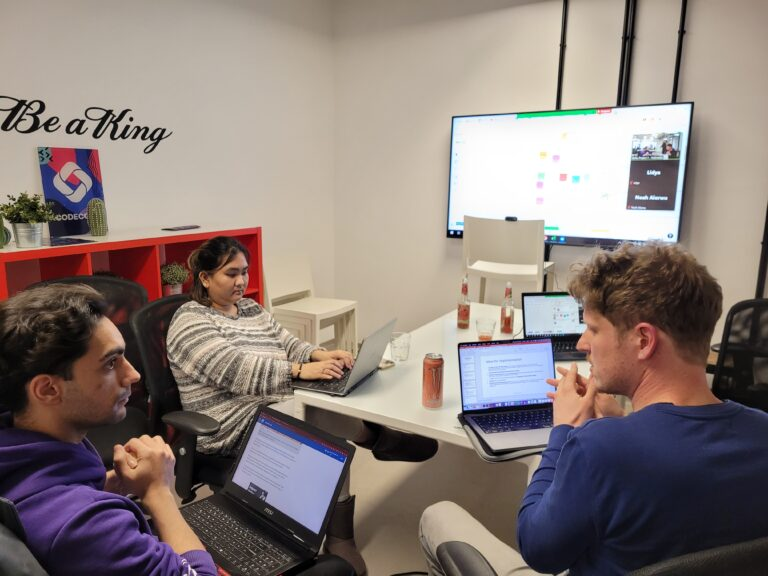
\includegraphics[width=1\textwidth]{pics/Project-forge-01.jpg}
    \caption{ICT4D.at Project-Forge Workshop 2022 (Wien)}
    \label{fig:Project-Forge-Workshop-2022}
\end{figure}

\begin{itemize}
    \item \textbf{ICT4D.at X RadioFarm Radio-Workshop (HTL Leonding):}
          \begin{itemize}
              \item \textbf{Anfang Juni 2023}
          \end{itemize}
\end{itemize}


Der Radio-Workshop bietet einen eineinhalbtägigen Kurs für Schülerinnen und Schüler der HTL-Leonding mit dem Schwerpunkt der Kompetenz- und Wissensvermittlung im Bereich der Kommunikation im Rahmen des Mediums Radio. Die Idee ist es, ein komplettes Radioprogramm nach den Interessen der SchülerInnen zu produzieren, wobei die Organisatoren vorschlagen, mit ihren Teammitgliedern international zusammenzuarbeiten. Das Team des Vereins ICT4D.at erstellt das gesamte Unterrichtsmaterial und vermittelt die Inhalte.

Die Schülerinnen und Schüler erstellen das Audiomaterial und präsentieren es selbst, aber die Partner des Vereins ICT4D.at können bei Bedarf zusätzliche Inhalte beisteuern (z.B. Interviews in Äthiopien). Die HTL Leonding wird versuchen, einige österreichische Politiker aus dem landwirtschaftlichen Bereich für eine kurze Interview-Session zu erreichen.

\begin{itemize}
    \item \textbf{Zielsetzung:}
\end{itemize}

Kompetenz- und Wissenstransfer durch die
gemeinsame Vorbereitung und Durchführung einer Fake-Live-Sendung am Ende eines Radioworkshops. Die Sendung kann später auf Radio FRO ausgestrahlt werden. 'Fake live' bedeutet, eine Live-Situation zu simulieren, ohne gleichzeitig live auf Sendung zu sein. Damit soll Authentizität erzeugt werden - Fehler werden in Kauf genommen und die Sendung wird später ausgestrahlt. Als zusätzliches Angebot kann Audiomaterial von unseren Kollegen in Afrika geplant und eingefügt werden, was dem Radioworkshop die Möglichkeit gibt, die internationale Zusammenarbeit und das interkulturelle Verständnis zu fördern.

Der Kurs ist für eine Klasse (max. 20 Teilnehmer) konzipiert und sollte in zwei Einheiten stattfinden: ein halber Tag für die grundlegende Einführung und Vorbereitung und ein ganzer Tag für die komplette Programmerstellung. Zwischen den beiden Einheiten sollte mindestens eine Woche Zeit liegen, damit Audiomaterial gesammelt werden kann.
Vorgeschlagene Termine:

\begin{itemize}
    \item {Basismodul: Anfang Juni, 2023 - nachmittag}
    \item {Workshoptag: Ende Juni, 2023 - ganztägig}
\end{itemize}

Um die Einbindung internationaler Kollegen zu ermöglichen, sollte der Workshop in englischer Sprache abgehalten werden. Die Schüler können selbst entscheiden, ob die Moderation ebenfalls auf Englisch oder auf Deutsch erfolgt.
Begleitende Lehrkraft
Eine Lehrkraft, die alle Teilnehmer kennt und den Workshopleiter unterstützt. Diese Lehrkraft ist vor Ort verfügbar und begleitet die Teilnehmer über einen Großteil des Workshops.

\begin{itemize}
    \item \textbf{Erwartete Ergebnisse:}
          \begin{itemize}
              \item {Alle Teilnehmer des Kurses schließen den Kurs erfolgreich ab und erhalten ein Zertifikat.}
              \item {Gemeinsame einstündige Radiosendung auf der Grundlage von selbst produziertem Audiomaterial}
              \item {Mit den erworbenen Fähigkeiten und Fertigkeiten können die TeilnehmerInnen ihre eigenen Radio- oder Podcast-Sendungen erstellen und wissen, wo sie diese verbreiten können.}
              \item {Die Teilnehmer haben auch interkulturelle Arbeitserfahrung gesammelt.}
          \end{itemize}
\end{itemize}

\begin{itemize}
    \item \textbf{Evaluation und Nachhaltigkeit:}
\end{itemize}

Ziel ist es, das im Workshop erstellte Programm zu veröffentlichen, z.B. auf Radio FRO. Die erstellte Sendung wird über die Kanäle von ICT4D.at beworben und kann auch als Podcast-Episode verbreitet werden. Mit den erworbenen Fähigkeiten können sich die Teilnehmer in Zukunft bei unabhängigen Radiosendern oder NGOs engagieren. Bei Interesse können sich die Teilnehmenden auch weiterhin in die Arbeit von ICT4D.at oder Radio FRO involvieren.

\begin{itemize}
    \item \textbf{UNESCO Internet4Trust Konferenz 2023 (Paris):}
          \begin{itemize}
              \item \textbf{23. Februar 2023}
          \end{itemize}
\end{itemize}

Die von der UNESCO organisierte Internet4Trust-Konferenz ist eine Veranstaltung zur Förderung von Vertrauen, Sicherheit und Gleichberechtigung im digitalen Raum. Die Konferenz dient als Plattform für den Dialog und die Zusammenarbeit zwischen verschiedenen Stakeholder, darunter Regierungen, Unternehmen des privaten Sektors, Organisationen der Zivilgesellschaft und Lehranstalten.

Das Hauptziel der Internet4Trust-Konferenz besteht darin, die Herausforderungen und Chancen zu diskutieren, die mit dem Aufbau eines vertrauenswürdigen digitalen Umfelds verbunden sind. Dazu gehören Diskussionen über Themen wie Datenschutz, Sicherheit, digitale Kompetenz und die moralische Anwendung von Technologie. Ziel der Konferenz ist es, Strategien, Politiken und Rahmenbedingungen zu entwickeln, die ein sicheres und integratives Online-Erlebnis für alle Internetbenutzer ermöglichen.

Arsham Edalatkhah wurde für die Rolle des WSA Youth Speaker Delegate nominiert, um die Stimme der Jugend während dieser Konferenz zu vertreten, da er am mPreneur Event in Ohrid teilgenommen und sehr gute Ergebnisse erzielt hat.

Der Grund, warum das WSA einen UNESCO-Jugenddelegierten wählen könnte, liegt in den gemeinsamen Werten und Zielen von WSA und UNESCO. Beide Organisationen legen großen Wert auf soziale Einflussnahme, insbesondere im Hinblick auf die Jugend. UNESCO-Jugenddelegierte sind junge Führungspersönlichkeiten, die sich in ihren Gemeinden engagieren und über die Fähigkeiten, die Erfahrung und die Leidenschaft verfügen, einen Beitrag zur globalen Diskussion über digitale Innovation und sozialen Wandel zu leisten.

Durch die Einbeziehung der UNESCO-Jugenddelegierten in den WSA kann die Organisation:

\begin{itemize}
    \item \textbf{Erwartete Ergebnisse:}
          \begin{itemize}
              \item {Das Wissen der Delegierten nutzen, um die Herausforderungen, mit denen junge Menschen in ihren Gemeinschaften konfrontiert sind, besser zu verstehen.}
              \item {Lernen, wie digitale Innovationen dazu beitragen können, die Bedürfnisse und Ziele junger Menschen zu erfüllen, insbesondere in den Bereichen Bildung, Wissensvermittlung und persönliche Entwicklung.}
              \item {Den Auswahlprozess vielfältiger und umfassender zu gestalten, indem Meinungen aus verschiedenen kulturellen, regionalen und wirtschaftlichen Hintergründen einbezogen werden.}
              \item {Verbesserung der Verbindung zwischen digitaler Innovation und den Zielen für nachhaltige Entwicklung, da die Delegierten mit diesen globalen Zielen vertraut sind.}
              \item {Förderung einer stärkeren Zusammenarbeit zwischen dem WSA, der UNESCO und anderen Organisationen, um digitale Innovationen für einen positiven sozialen Wandel, nachhaltige Entwicklung und die Stärkung der Jugend zu fördern.}
          \end{itemize}
\end{itemize}


Für Arsham Edalatkhah war es wichtig, den Experten auf dem Podium keine Fakten und Statistiken zu erzählen, die ihnen bereits bekannt sind. Stattdessen nutzte er die Gelegenheit, um die Unterschiede zwischen den Generationen zu beleuchten und darauf hinzuweisen, wie wichtig es ist, die Jugend durch Peer-to-Peer-Trainings über das Thema Digitalisierung und soziale Medien aufzuklären. Er selber hat bereits Erfahrung mit diesem Thema, da er selbst die Peer-Trainings an der HTL Leonding absolviert hat und den jüngeren Schülern der HTL Leonding Unterstützung bietet.

Auch in der NMS-Hart in Leonding hält er Vorträge über die Gestaltung der Kommunikation in sozialen und virtuellen Dynamiken und wie dadurch die Klassengemeinschaft gestärkt wird. So erzählte er den 1000 Zuschauern der Jugendkonferenz von seinen diesbezüglichen Erfahrungen. Er erwähnte, dass er eine große Differenz zwischen den Schülern und ihren Lehrern sah, wenn es um die digitale Dynamik geht, und dass er den Lehrern half, diese Lücke zu schließen, indem er den Schülern eine Art Betreuung für die Schulklasse ermöglichte.

Die Rolle der Jugend spielt im Rahmen der Internet4Trust-Konferenz eine wichtige Rolle. Als digitale 'Natives' sind junge Menschen oft am stärksten von der sich schnell verändernden digitalen Welt betroffen. Ihre Perspektiven und Erfahrungen sind von unschätzbarem Wert, wenn es darum geht, den aktuellen Stand des Vertrauens im digitalen Raum zu verstehen und die Bereiche zu ermitteln, die verbessert werden müssen. Durch die Einbindung der Jugendlichen in die Konferenz können sie zum Diskurs und zum Entscheidungsprozess beitragen und so die Zukunft des Internets mitbestimmen.


Die Rolle der Jugend auf der Internet4Trust-Konferenz umfasst die folgenden Punkte:

\begin{itemize}
    \item \textbf{Die Rolle der Jugend auf der Internet4Trust-Konferenz umfasst die folgenden Punkte:}
          \begin{itemize}
              \item {Weitergabe ihrer Erfahrungen und Einsichten in Bezug auf Vertrauen und Sicherheit in der digitalen Welt.}
              \item {Teilnahme an Workshops und Podiumsdiskussionen, die ihnen eine Plattform bieten, um ihre Sorgen, Ideen und Lösungen zu äußern.}
              \item {Kontaktaufnahme mit Entscheidungsträgern und Interessenvertretern aus verschiedenen Bereichen, um einen generationenübergreifenden Austausch zu ermöglichen.}
              \item {Unterstützung bei der Entwicklung und Förderung von Programmen zur Förderung der digitalen Bildung, die sicherstellen, dass junge Menschen in der Lage sind, sich sicher und verantwortungsvoll im digitalen Raum zu bewegen.}
              \item {Förderung eines globalen Gemeinschaftsgefühls durch den Kontakt mit Jugendlichen unterschiedlicher Herkunft und Kultur, um das gegenseitige Vertrauen und den Respekt zu fördern.}
          \end{itemize}
\end{itemize}

\begin{figure}[H]
    \centering
    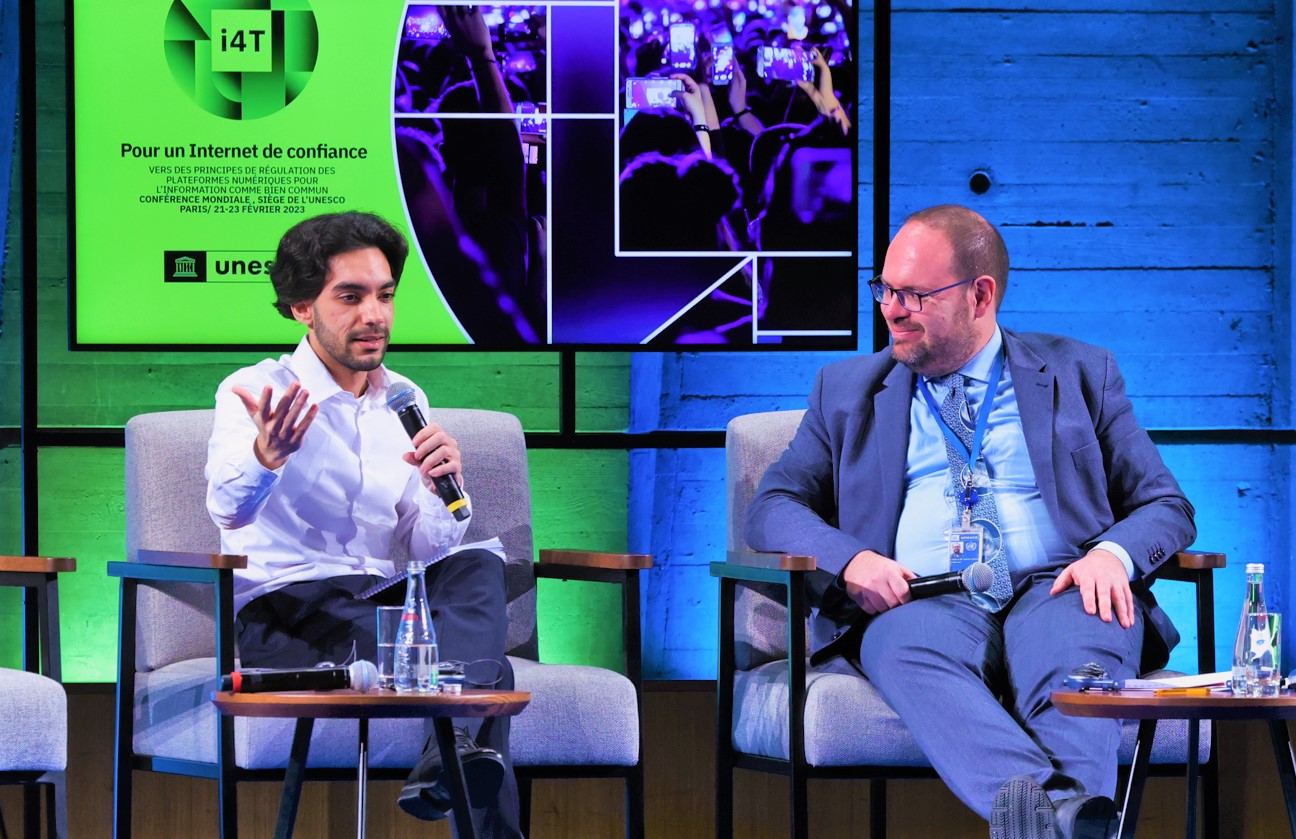
\includegraphics[width=1\textwidth]{pics/unesco-internet4trust-2023.jpg}
    \caption{UNESCO Internet4Trust Konferenz 2023 (Paris):}
    \label{fig:unesco-internet4trust-2023}
\end{figure}

\begin{itemize}
    \item \textbf{Spusu Innovation Award (Wien):}
          \begin{itemize}
              \item \textbf{22. März 2023}
          \end{itemize}
\end{itemize}

Der Spusu Innovation Award ist ein bedeutendes Preisverleihungsprogramm, das in Österreich, insbesondere in Wien, organisiert wird. Mit dem Preis werden herausragende Innovationen, revolutionäre Technologien und revolutionäre Lösungen in verschiedenen Bereichen ausgezeichnet. Der Spusu Innovation Award wird von Spusu, einem Mobilfunkbetreiber in Österreich, organisiert und gesponsert.

Österreich blickt auf eine reiche Innovations- und Technologiegeschichte zurück, und die Hauptstadt Wien ist ein wichtiger Standort für verschiedene Branchen. Mit der Verleihung von Preisen wie dem Spusu-Innovationspreis will das Land kreative Köpfe und Unternehmen ermutigen, sich weiterzuentwickeln und zum Wirtschaftswachstum der Region beizutragen.

Die Innovationspreise konzentrieren sich auf die folgenden Kategorien:

\begin{itemize}
    \item {Wissenschaft und Technologie}
    \item {Kunst und Kultur}
    \item {Umwelt und Nachhaltigkeit}
    \item {Gesundheit und Wohlbefinden}
\end{itemize}

Die Gewinner des Spusu-Innovationspreises erhalten Anerkennung, Vernetzungsmöglichkeiten und finanzielle Unterstützung, damit sie ihre innovativen Ideen weiterentwickeln und auf den Markt bringen können. Diese Art von Preisen ist für die Förderung einer Innovationskultur und die Unterstützung des Wachstums der lokalen Wirtschaft von wesentlicher Bedeutung.

Das Team Nochba erreichte bei diesem Wettbewerb den dritten Platz in der Kategorie soziale Innovation und gewann insgesamt 500 €.

\begin{figure}[H]
    \centering
    \includegraphics[width=1\textwidth]{pics/spusu-InnovationAward-2023.jpg}
    \caption{Spusu Innovation Award 2023 (Wien)}
    \label{fig:spusu-InnovationAward-2023}
\end{figure}

\begin{itemize}
    \item \textbf{World Summit Award (Graz)}
          \begin{itemize}
              \item \textbf{26. bis 28. April 2023}
          \end{itemize}
\end{itemize}

Der World Summit Award (WSA) in Graz ist ein angesehener internationaler Wettbewerb, der hervorragende digitale Innovationen mit einem starken Fokus auf soziale Aspekte auszeichnet und diese unterstützt. Der WSA findet jährlich in Graz statt und hat das Ziel, die digitale Kluft zu überbrücken, nachhaltige Entwicklung zu fördern und Einzelpersonen und Gemeinschaften durch Technologie zu stärken. Die Veranstaltung bringt eine vielfältige Gruppe von Stakeholdern zusammen, darunter Unternehmer, Innovatoren, Behördenvertreter, Investoren und zivilgesellschaftliche Organisationen, und fördert so ein Umfeld der Zusammenarbeit und des gegenseitigen Informationsaustausches.

Stakeholder:

\begin{itemize}
    \item {Unternehmer und Innovatoren:}
          \begin{itemize}
              \item {Der WSA bietet kreativen Köpfen eine Plattform, um ihre digitalen Lösungen zu präsentieren, ihre Netzwerke zu erweitern und internationale Anerkennung zu finden.}
          \end{itemize}
    \item {Behördenvertreter:}
          \begin{itemize}
              \item {Sie beteiligen sich an politischen Diskussionen, identifizieren potenzielle Kooperationen und unterstützen Projekte, die zu nationalen und globalen Entwicklungsplänen beitragen.}
          \end{itemize}
    \item {Investoren:}
          \begin{itemize}
              \item {Der WSA bietet eine einzigartige Gelegenheit für Investoren, vielversprechende digitale Innovationen zu identifizieren, Partnerschaften zu schließen und in Projekte mit großer sozialer Wirkung zu investieren.}
          \end{itemize}
    \item {Organisationen der Zivilgesellschaft:}
          \begin{itemize}
              \item {Diese Gruppen nehmen am WSA teil, um Projekte zu unterstützen, die mit ihren Aufgaben übereinstimmen, und um Kooperationen für einen größeren sozialen Fortschritt zu erleichtern.}
          \end{itemize}
\end{itemize}

Zielsetzung:

Das Hauptziel des World Summit Award ist es, digitale Innovationen zu identifizieren und zu fördern, die das Potenzial haben, das Leben der Menschen zu verbessern, sich mit aktuellen gesellschaftlichen Herausforderungen auseinanderzusetzen und zur Erreichung der Ziele für nachhaltige Entwicklung der Vereinten Nationen (SDGs) beizutragen. Durch die Anerkennung und Auszeichnung der Leistungen dieser Entwickler möchte der WSA mehr Menschen dazu inspirieren, Technologie als Werkzeug für positive Veränderungsmaßnahmen zu nutzen.

Qualifikationskriterien:

Um sich für den World Summit Award zu qualifizieren, muss ein Projekt die folgenden Aspekte erfüllen:

\begin{itemize}
    \item {Eine starke soziale Wirkung und die Ausrichtung auf eines oder mehrere der SDGs der Vereinten Nationen nachweisen.}
    \item {Es muss sich um eine digitale Innovation handeln, beispielsweise eine mobile App, eine Website, eine Plattform oder eine Softwarelösung.}
    \item {Es muss innerhalb der letzten zwei Jahre eingeführt, entwickelt oder erheblich aktualisiert worden sein.}
    \item {Sie müssen vom Projekteigentümer oder einem autorisierten Vertreter eingereicht werden.}
    \item {Sie müssen in einer der acht offiziellen Kategorien des WSA präsentiert werden:}
          \begin{itemize}
              \item {Regierung und Bürgerschaftliches Engagement}
              \item {Gesundheit und Wohlbefinden}
              \item {Lernen und Bildung}
              \item {Umwelt und Erneuerbare Energien}
              \item {Kultur und Tourismus}
              \item {Smarte Urbanisierung und Immobilien}
              \item {Wirtschaft und Handel}
              \item {Integration und gesellschaftliche Ermutigung}
          \end{itemize}
\end{itemize}

\begin{itemize}
    \item \textbf{Vorteile für die Gewinner:}
\end{itemize}

Die Preisträger des World Summit Award erhalten zahlreiche Vorteile, darunter:

\begin{itemize}
    \item {Internationale Anerkennung:}
          \begin{itemize}
              \item {Die Siegerprojekte werden auf der globalen Plattform des WSA vorgestellt und gewinnen dadurch an Sichtbarkeit und Relevanz.}
          \end{itemize}
    \item {Gelegenheiten zum Networking:}
          \begin{itemize}
              \item {Die Gewinner haben die Möglichkeit, auf dem WSA Global Congress mit anderen Innovatoren, Investoren und Interessengruppen in Kontakt zu treten.}
          \end{itemize}
    \item {Mentoring und Erweiterung der Fachkenntnisse:}
          \begin{itemize}
              \item {Die Gewinner erhalten fachkundige Beratung, Workshops und Schulungen, die ihnen dabei helfen, ihre Projekte zu erweitern und ihre Erfolge zu maximieren.}
          \end{itemize}
    \item {Zugang zu Ressourcen:}
          \begin{itemize}
              \item {Die Gewinner können auf das umfangreiche Netzwerk des WSA an Partnern, Experten und Ressourcen zurückgreifen, um das Wachstum und die Entwicklung ihrer Projekte zu unterstützen.}
          \end{itemize}
\end{itemize}

Durch die Teilnahme am World Summit Award in Graz können digitale Innovatoren ihre Projekte aufwerten, zu einer globalen sozialen Wirkung beitragen und Teil einer lebendigen Gemeinschaft werden, die sich der Nutzung von Technologie für das Allgemeinwohl verpflichtet hat.

Das Projekt Nochba hat sich erfolgreich für den hoch geschätzten World Summit Award in der Kategorie 'Soziale Innovation' qualifiziert. Grund dafür sind die starken sozialen Aspekte der App und ihr bedeutender Beitrag zu den Zielen für nachhaltige Entwicklung der Vereinten Nationen (SDGs).

Der innovative Ansatz und das Engagement des Nochba-Teams bei der Bewältigung aktueller gesellschaftlicher Herausforderungen haben ihnen die Möglichkeit verschafft, ihre zukunftsorientierte Lösung auf der globalen Bühne des WSA vor einem Publikum von über 1.000 internationalen Teilnehmern zu präsentieren.

Indem sie ihre Vision und ihre Errungenschaften einem breit gefächerten Publikum aus Unternehmern, Behördenvertretern, Investoren und zivilgesellschaftlichen Organisationen vorstellen, hat das Nochba-Team die Gelegenheit, nicht nur andere zu inspirieren, sondern auch sein Netzwerk zu erweitern und strategische Partnerschaften zu formen.

Auf dieser Plattform können sie das Potenzial ihrer App demonstrieren, um positive Veränderungen voranzutreiben, die soziale Entwicklung zu fördern und skalierbare Lösungen im Einklang mit den übergreifenden Zielen des World Summit Award zu entwickeln.

Die Teilnahme von Project Nochba am WSA Global Congress wird zweifellos die Sichtbarkeit und den Ruf des Projekts deutlich schärfen und den Weg für eine verstärkte Zusammenarbeit, Investitionen und Unterstützung öffnen, um die Auswirkungen auf die Gemeinschaften weltweit weiter zu verstärken. Durch die Nutzung der zahlreichen Möglichkeiten und Ressourcen des WSA ist das Nochba-Team gut positioniert, um einen dauerhaften Unterschied zu machen und einen Beitrag zur globalen Agenda für nachhaltige Entwicklung zu leisten.

\begin{itemize}
    \item \textbf{Project Awards an der HTL Leonding}
          \begin{itemize}
              \item \textbf{28. März 2023}
          \end{itemize}
\end{itemize}

Das Team Nochba nahm an den Project Awards an der HTL Leonding teil, einer renommierten technischen Schule in Oberösterreich, die Schüler in verschiedenen Bereichen wie Elektronik, Informatik, Mechatronik und Medientechnik ausbildet. Der Wettbewerb bietet Schülern die Chance, ihre Fähigkeiten und Ideen zu präsentieren, wertvolles Feedback von Experten zu erhalten und möglicherweise Preise zu gewinnen.

Obwohl das Projekt Nochba sehr innovativ und beeindruckend ist, schaffte das Team es leider nicht ins Finale. Die Jury stellte fest, dass das Team bereits mehrere Auszeichnungen gewonnen hat und das Projekt im Vergleich zu anderen Teilnehmern überqualifiziert ist. Allerdings hat die Jury ein eigenes Set von Werten und Projekten, nach denen sie suchen, und da die Nochba-App eine Social Media App ist, ist es möglicherweise besser für andere Projekte, in diesem Wettbewerb anzutreten.

Trotzdem hat das Team durch die Teilnahme an diesem Wettbewerb wertvolle Erfahrungen gesammelt und ihre Fähigkeiten in den technischen Disziplinen weiterentwickelt.

\begin{figure}[H]
    \centering
    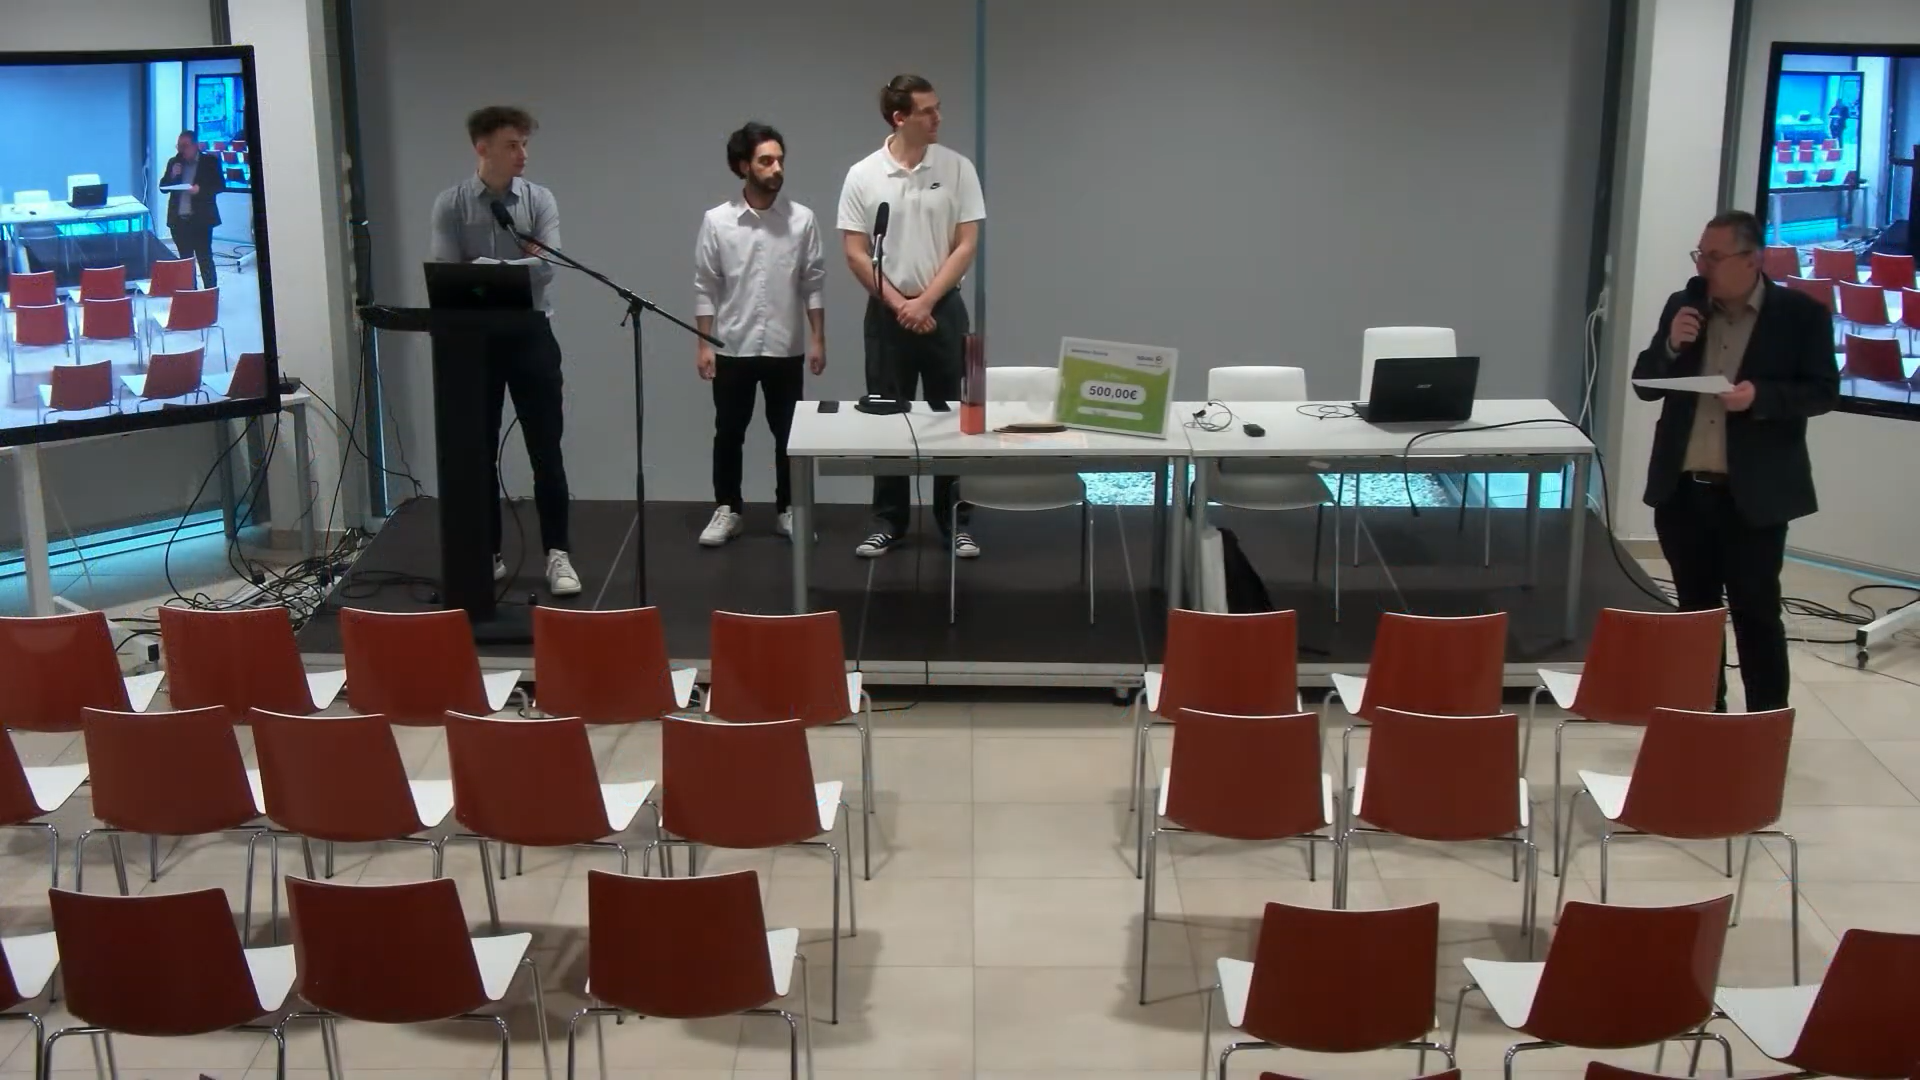
\includegraphics[width=1\textwidth]{pics/ProjectAward.png}
    \caption{Project Awards an der HTL Leonding 2023}
    \label{fig:ProjectAward}
\end{figure}

\begin{itemize}
    \item \textbf{Hochladen von 'Nochba' in den Play Store als Early-Access-App}
          \begin{itemize}
              \item \textbf{22. März 2023}
          \end{itemize}
\end{itemize}

Die Entwicklung einer App umfasst mehrere Phasen, und es muss sichergestellt werden, dass ihre Funktionalität und Benutzerfreundlichkeit den gewünschten Standards entsprechen, bevor sie vollständig veröffentlicht wird. Um dies zu erreichen, hat das Team Nochba die App 'Nochba' als Early Access App zu Testzwecken in den Google Play Store hochgeladen. Auf diese Weise konnten die Nutzer wertvolles Feedback geben und Fehler oder Probleme identifizieren, die behoben werden mussten. Im Folgenden finden Sie einen Überblick über die Schritte, die das Team Nochba beim Hochladen von 'Nochba' in den Play Store als Early-Access-App unternommen hat:

\begin{itemize}
    \item \textbf{Vorbereiten der App für die Veröffentlichung}
          \begin{itemize}
              \item {Das Team Nochba bereitete die App für die Freigabe vor, indem es sicherstellte, dass sie voll funktionsfähig war und alle erforderlichen Elemente wie Symbole, Screenshots und Materialien für die Präsentation zusammenstellte. Das Team entfernte alle Platzhalter oder Testdaten und bestätigte, dass die App den Richtlinien des Google Play-Entwicklerprogramms und der Vertriebsvereinbarung für Entwickler erfüllt.}
          \end{itemize}
    \item \textbf{Anmeldung für ein Google Play-Entwicklerkonto}
          \begin{itemize}
              \item {Das Team Nochba meldete sich für ein Google Play-Entwicklerkonto an, wofür eine einmalige Registrierungsgebühr von 25 € anfiel. Diese Gebühr wird von Google erhoben, um die Identität des Entwicklers zu überprüfen und die Qualität und Sicherheit der auf der Plattform veröffentlichten Apps zu gewährleisten. Durch die Zahlung der Gebühr erhielt das Team Nochba Zugang zur Google Play Console, wo es die Veröffentlichung und Verbreitung der App verwaltete. Die Registrierungsgebühr hilft Google auch, die Kosten für die Verwaltung der Plattform zu decken und sicherzustellen, dass sie ein nachhaltiger und zuverlässiger Marktplatz für Entwickler und Nutzer bleibt.}
          \end{itemize}
    \item \textbf{Einrichten der App in der Google Play-Konsole}
          \begin{itemize}
              \item {In der Google Play-Konsole richtete das Team Nochba die App ein, indem es die erforderlichen Informationen angab, z. B. den Namen der App, die Standardsprache und den Anwendungstyp, und die entsprechende Preisoption auswählte.}
          \end{itemize}
    \item \textbf{Vorbereiten des App-Store-Listings}
          \begin{itemize}
              \item {Das Team Nochba bereitete die Auflistung der App im Store vor, indem es alle erforderlichen Details bereitstellte, darunter eine Kurzbeschreibung, eine detaillierte Beschreibung, Screenshots, eine Grafik zu den Funktionen und ein App-Symbol, um sicherzustellen, dass die Assets der App den Richtlinien und Spezifikationen von Google Play entsprechen.}
          \end{itemize}
    \item \textbf{Konfigurieren der Inhaltsbewertung der App}
          \begin{itemize}
              \item {Das Team Nochba konfigurierte die Inhaltseinstufung der App, indem es den Fragebogen zur Inhaltseinstufung ausfüllte und so sicherstellte, dass die App der richtigen Zielgruppe angezeigt wurde. In diesem Fall entschied das Team, dass die Nutzer der App mindestens 14 Jahre alt sein sollten, da solche Apps mit diesem Grad an Komplexität und sozialem Aspekt ein gewisses Maß an Reife erfordern, um verantwortungsvoll genutzt zu werden.}
          \end{itemize}
    \item \textbf{Vorbereiten der App für Alpha- oder Beta-Tests}
          \begin{itemize}
              \item {Im Bereich 'Testen' der Play Console bereitete das Team Nochba die App für Alpha- oder Betatests vor, indem sie eine Testversion erstellten und die APK- oder App-Bundle-Datei der App heraufluden. Außerdem fügten sie alle erforderlichen Informationen hinzu, beispielsweise die Versionshinweise.}
          \end{itemize}
    \item \textbf{Hinzufügen von Testern und Einladung zum Testen der App}
          \begin{itemize}
              \item {Das Team Nochba fügte Tester hinzu und übermittelte ihnen eine Einladung zum Testen der App, indem es die Testmethode (geschlossener oder offener Test) auswählte und den Testern entweder ihre E-Mail-Adressen oder eine URL für den offenen Test zur Verfügung stellte. Das Team informierte die Tester darüber, dass sie Nochba als Early-Access-App über den angegebenen Link aus dem Play Store herunterladen konnten.}
          \end{itemize}
    \item \textbf{Überprüfen und Veröffentlichen der App}
          \begin{itemize}
              \item {Schließlich überprüfte und veröffentlichte das Team Nochba die App. Nachdem sie alle Informationen und Assets überprüft hatten, klickten das Team auf 'Überprüfen und veröffentlichen', um die App zur Überprüfung einzureichen. Der Überprüfungsprozess nahm mehrere Tage in Anspruch. Danach wurde die App im Play Store als Early Access-App zu Testzwecken zur Verfügung gestellt.}
          \end{itemize}
\end{itemize}

Mit diesen Schritten hat das Team Nochba erfolgreich eine Early-Access-App in den Play Store hochgeladen, um wertvolles Feedback von Testern zu sammeln und die Performance und Benutzerfreundlichkeit der App vor dem eigentlichen Start zu verfeinern.

\begin{figure}[H]
    \centering
    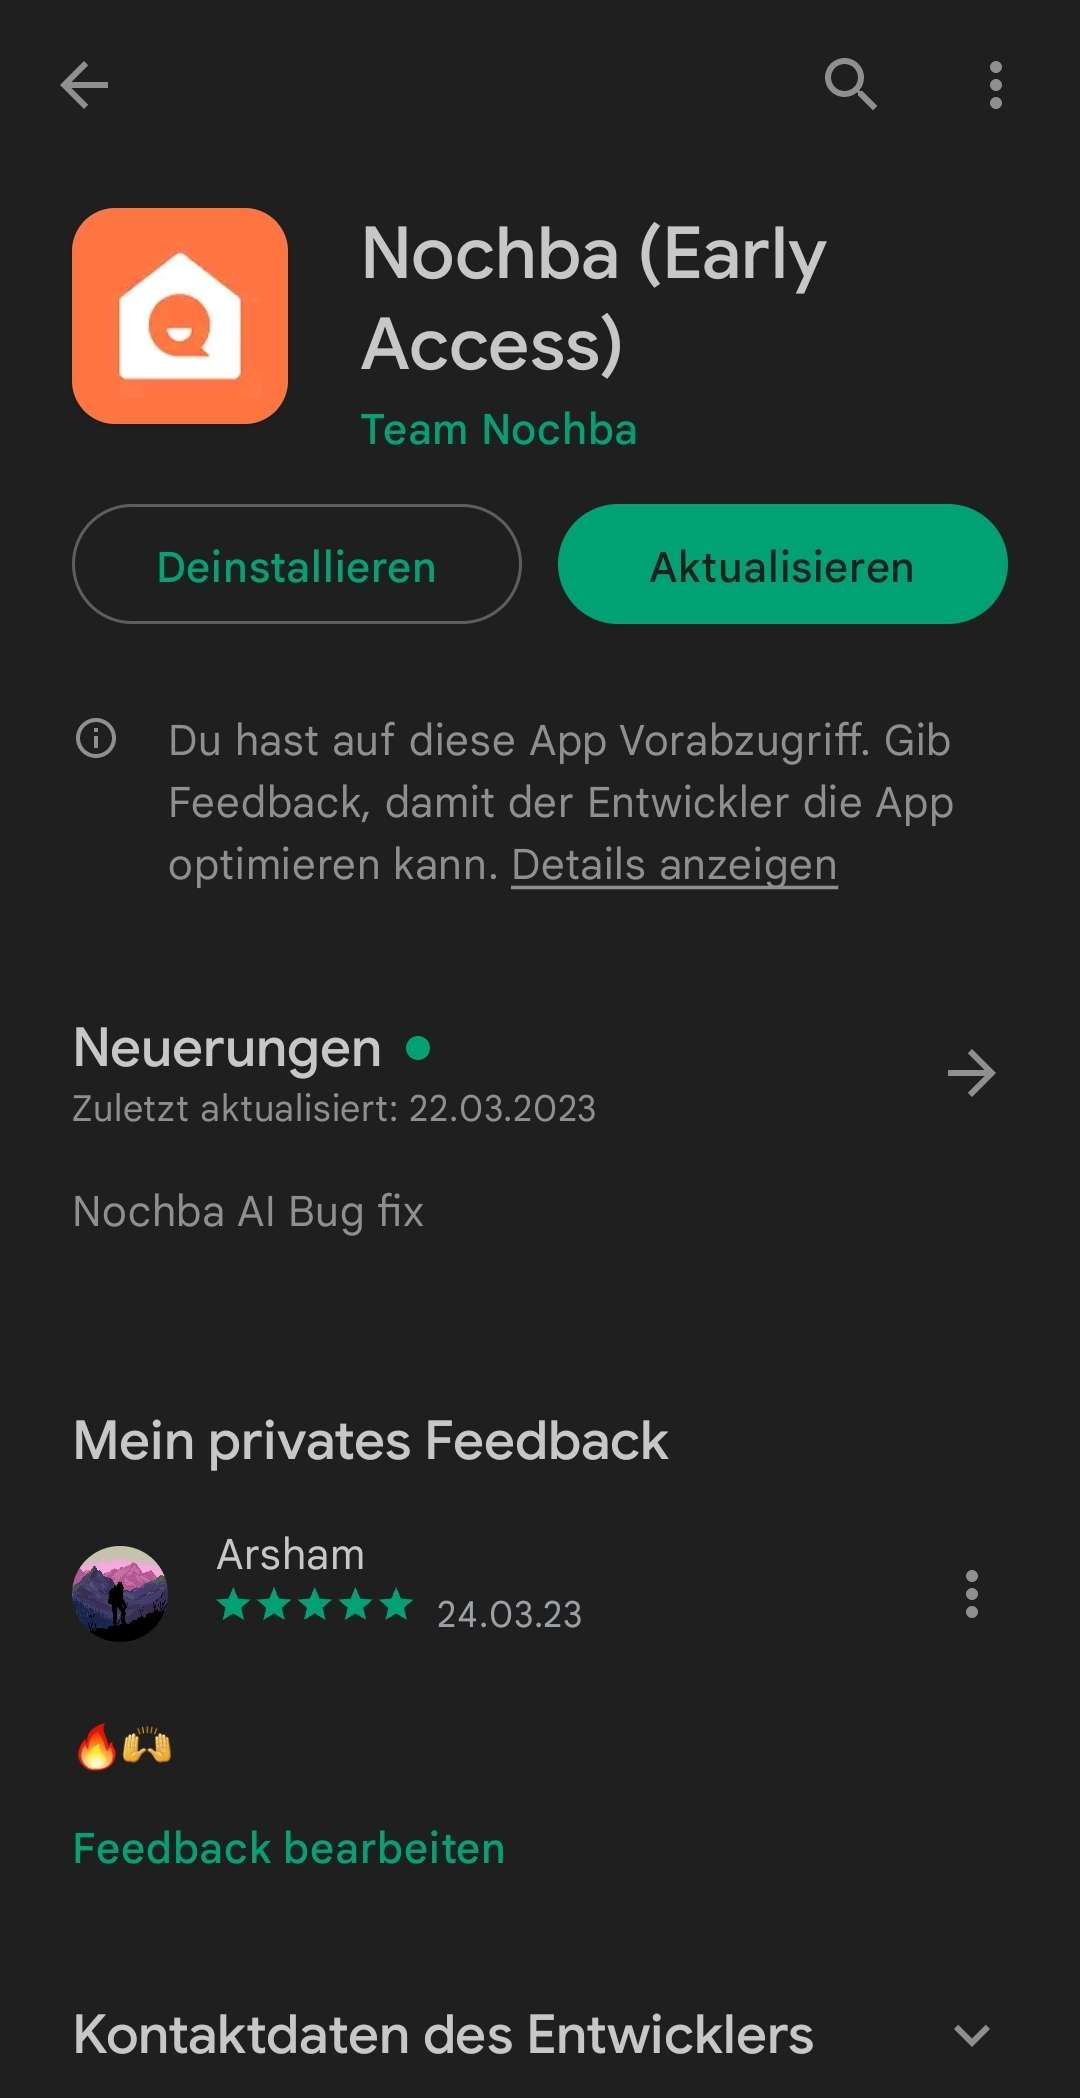
\includegraphics[width=0.3\textwidth]{pics/Nochba-Google_Play_Store.jpg}
    \caption{Screenshot der Nochba-App im Google Play Store}
    \label{fig:Nochba-GooglePlayStore}
\end{figure}

\section{Projektvorgehensmodell}
\subsection{Projektorganisation}

\subsubsection{Discord}
\setauthor{Martin Hausleitner}
Die primäre Kommunikationsplattform zwischen dem Team und den Diplomarbeitbetreuer ist Discord. Da die Arbeit in den Sommerferien 2022 begonnen hat und zu diesem Zeitpunkt Corona-Regelungen galten, musste eine Meeting-Plattform gefunden werden, die sowohl Video- als auch Text-Chat ermöglicht. Aufgrund der Vertrautheit mit Discord und der Tatsache, dass es kostenlos ist, fiel die Entscheidung leicht.

Während der Diplomarbeit wurden über 40 Text-Kanäle erstellt, um alle relevanten Informationen, Notizen und Dokumentation zu speichern. Die Meeting-Notizen wurden jedoch auf ClickUp gespeichert.
\subsubsection{ClickUp}
\setauthor{Martin Hausleitner}
Um das Projekt effizient zu organisieren, wird nicht nur eine WhatsApp-Gruppe genutzt, sondern auch das Projektmanagement-Tool ClickUp. Die Entscheidung für ClickUp fiel leicht, da bereits viele Projektmanagement-Programme ausprobiert wurden und ClickUp bei den letzten Projekten am besten abgeschnitten hat. Außerdem ist es sehr intuitiv und einfach zu erlernen, was von beiden Teammitgliedern bestätigt wird.

\begin{figure}[h]
    \centering
    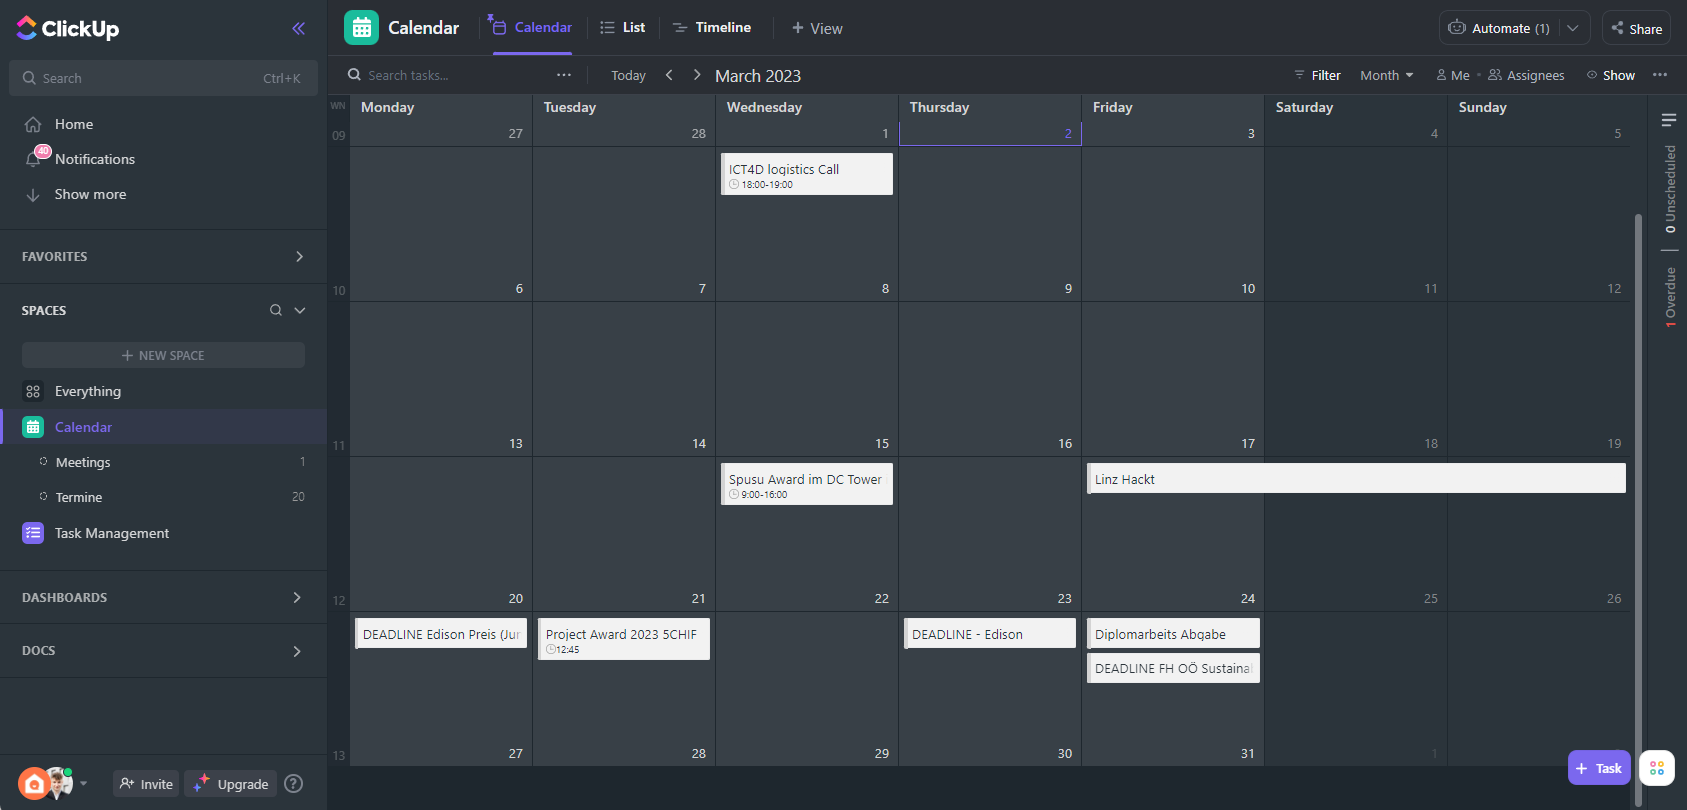
\includegraphics[width=1\textwidth]{./pics/clickup-calender-view.png}
    \caption{ClickUp Dashboard Kalender}
    \label{fig:clickup-calendar}
\end{figure}


In der Diplomarbeit wurden viele Mentoring-Sessions, Meetings mit dem Diplomarbeitbetreuer und weitere Termine wie Wettbewerbe vereinbart. Ohne eine geeignete Methode zur Verwaltung all dieser Termine kann es schnell unübersichtlich werden. Deshalb wurde das Kalender-Feature von ClickUp genutzt, um alle Einträge abzubilden, wie in Abbildung \ref{fig:clickup-calendar} zu sehen ist. Der Kalender wurde automatisch mit den persönlichen Kalendern synchronisiert, wie beispielsweise einem Google Kalender. Dadurch wurden nie Termine verpasst, was insbesondere dem Projektleiter sehr geholfen hat, da er nicht jeden daran erinnern musste, alle Termine in seinem Kalender einzutragen.

Ein weiterer wichtiger Punkt war das Task-Management in dem Projekt. Da im Projekt schnell viele Aufgaben koordiniert werden mussten, war es sinnvoll, alle Aufgaben in einer simplen To-Do-Liste abzubilden. Vor den Semesterferien wurde beispielsweise eine eigene Abteilung für Ferien-Tasks erstellt, um einen Überblick über alle Aufgaben während der Semesterferien zu haben. Obwohl die Tasks-To-Listen nicht aktiv genutzt wurden, war es sehr praktisch, um den Fortschritt zu überwachen und sicherzustellen, dass alles rechtzeitig erledigt wurde.

Zusammenfassend war ClickUp eine große Bereicherung für das
Projektmanagement, da es viel Zeit bei der Verwaltung von
Terminen und Aufgaben gespart hat. Auch die Benutzung als
neuer Benutzer war sehr einfach, sodass keine lange
Einarbeitungszeit nötig war. Besonders faszinierend ist,
dass ClickUp sehr intuitiv ist und viele nützliche Features
bietet.



\begin{spacing}{1}
	\chapter{Technologien}\label{chapter:tech}
\end{spacing}
\setauthor{Martin Hausleitner}
\section{Technologieevaluierung}

Ein zentraler Aspekt jedes Projektbeginns ist die Evaluierung der Technologie. Wir haben uns bewusst viel Zeit genommen, um eine schnelle und unkomplizierte Entwicklung zu ermöglichen und später mögliche Bedauern zu vermeiden. Die Anforderungen für das Projekt umfassen die Erstellung von iOS- und Android-Apps sowie möglicherweise einer Web-App in Zukunft. Hinsichtlich des Backends ist für uns insbesondere die Unterstützung von Geopoints und Geo-Queries in der Datenbank von Bedeutung. Idealerweise sollte das System zudem eine integrierte Authentifizierungsfunktion aufweisen.


\subsection{Frontend}

Im Bereich der Frontend-App-Entwicklung stehen verschiedene Möglichkeiten zur Verfügung, um eine App zu programmieren. Eine Option besteht darin, eine nativ programmierte iOS- oder Android-App zu erstellen. Allerdings haben wir uns als Team schnell gegen diese Option entschieden, da keiner von uns mit einer der Plattformen vertraut ist und dies zu einem erheblichen Mehraufwand führen würde. Dies würde bei einem kleinen Team von nur drei Personen zu viel Zeit in Anspruch nehmen. Ein Vorteil der nativen Programmierung besteht jedoch darin, dass man auf alle nativen APIs zugreifen kann und die Performance besser ist, da die Entwickler der App-Schnittstelle vom Hersteller des Betriebssystems stammen.

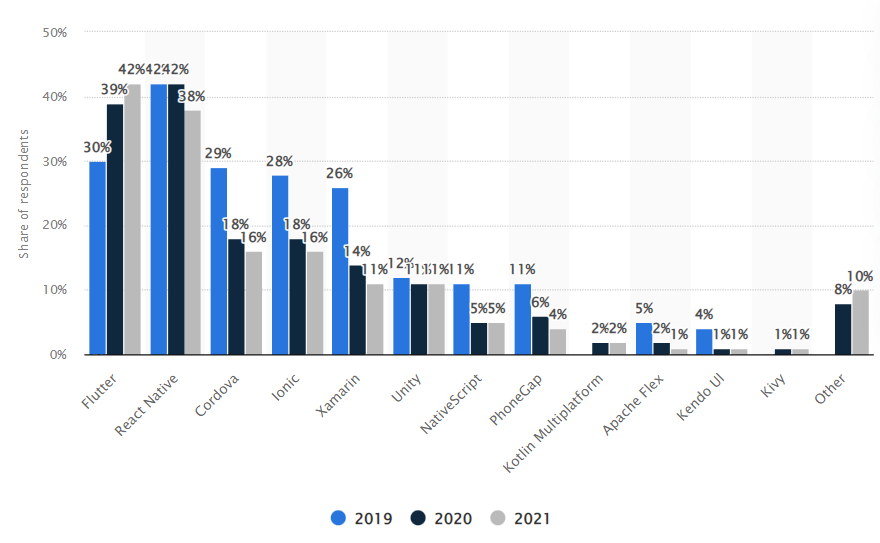
\includegraphics[width=0.75\textwidth]{pics/cross-platform-statisitics.png}

https://www.statista.com/statistics/869224/worldwide-software-developer-working-hours/

Um eine effektive und plattformübergreifende Entwicklung zu gewährleisten, haben wir uns dazu entschieden, ein Cross-Platform-Framework zu verwenden. Wir haben die Statistik darüber betrachtet, welche Plattformen am meisten genutzt werden und dabei festgestellt, dass Flutter mit 42 Prozent das meistgenutzte Framework ist und die Tendenz steigend ist. Auf Platz 2 liegt React Native, das fast genauso beliebt ist.

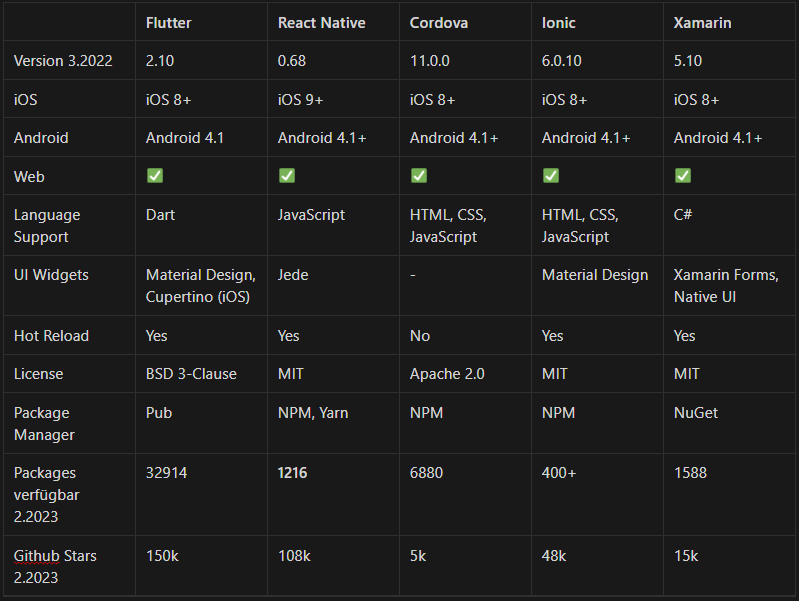
\includegraphics[width=0.75\textwidth]{pics/temp-table.png}

% |  | Flutter | React Native | Cordova | Ionic | Xamarin |
% | --- | --- | --- | --- | --- | --- |
% | Version 3.2022 | 2.10 | 0.68 | 11.0.0 | 6.0.10 | 5.10 |
% | iOS | iOS 8+ | iOS 9+ | iOS 8+ | iOS 8+ | iOS 8+ |
% | Android | Android 4.1 | Android 4.1+ | Android 4.1+ | Android 4.1+ | Android 4.1+ |
% | Web | Ja | Ja | Ja | Ja | Ja |
% | Language Support | Dart | JavaScript | HTML, CSS, JavaScript | HTML, CSS, JavaScript | C Sharp |
% | UI Widgets | Material Design, Cupertino (iOS) | Jede | - | Material Design | Xamarin Forms, Native UI |
% | Hot Reload | Yes | Yes | No | Yes | Yes |
% | License | BSD 3-Clause | MIT | Apache 2.0 | MIT | MIT |
% | Package Manager | Pub | NPM, Yarn | NPM | NPM | NuGet |
% | Packages verfügbar 2.2023 | 32914 | 1216 | 6880 | 400+ | 1588 |
% | Github Stars 2.2023 | 150k | 108k | 5k | 48k | 15k |

Quellen:
[https://reactnative.directory/](https://reactnative.directory/)

[https://pub.dev/](https://pub.dev/)
[https://www.npmjs.com/search?q=keywords:ecosystem:cordova](https://www.npmjs.com/search?q=keywords:ecosystem:cordova)
[https://github.com/xamarin](https://github.com/xamarin)
[https://github.com/apache/cordova-android](https://github.com/apache/cordova-android)

[https://ionic.io/docs/supported-plugins](https://ionic.io/docs/supported-plugins)

[https://market.ionicframework.com/plugins](https://market.ionicframework.com/plugins)

In der Vergleichstabelle haben wir die wichtigsten Informationen zu den verschiedenen Frameworks zusammengefasst. Dabei haben wir festgestellt, dass alle Plattformen unsere Anforderungen erfüllen. Xamarin hat für uns als Team, das seit Jahren C Sharp programmiert, ein gewisses Interesse geweckt. Allerdings hat Dart eine ähnliche Syntax wie C Sharp, weshalb es für uns als Team auch eine geeignete Option darstellt.

Flutter hat als UI-Widget-Library sowohl Material Design 2 und 3 als auch eine iOS Library, die das native iOS-Design 1:1 abbildet. Dadurch kann der Nutzer den Unterschied zwischen nativen und Flutter-Designs kaum erkennen. Xamarin hat ebenfalls eine UI-Library namens Xamarin.Forms, die auf allen Plattformen funktioniert und native UI-Libraries für jede Plattform enthält.

React Native ist zwar in JavaScript geschrieben, aber man kann keine React-Komponenten importieren und verwenden. Wenn man jedoch bereits Erfahrung mit React.js hat, kann man sich als Entwickler leichter in React Native einarbeiten. Die letzten beiden Plattformen Cordova und Ionic basieren auf HTML, CSS und JavaScript, was den Vorteil bietet, dass man auf jede JavaScript-Library zugreifen kann.

Ein wichtiger Faktor bei der Wahl des Frameworks ist auch der Hot Reload. Cordova bietet diese Funktion nicht, alle anderen Plattformen hingegen schon, was für uns ein dealbreaker ist.

Die Package-Manager wurden ebenfalls verglichen und der von Flutter hat uns am meisten überzeugt, da jedes Package ein Beispiel hat und man anhand von Pub Points sehen kann, wie gut das Package in verschiedenen Kriterien abschneidet. Zudem kann man sehen, welche Plattformen das Package unterstützt.

Obwohl npm der meistgenutzte Package-Manager ist, ist er nicht spezifisch auf ein bestimmtes Framework ausgerichtet und es fehlen einige Funktionen, die Pub hat. NuGet kennen wir bereits von der CSharp-Entwicklung und unserer Meinung nach wirkt er sehr altmodisch und fehlt ebenfalls einige Funktionen, die Pub hat.

Ein weiterer wichtiger Faktor bei der Wahl des Frameworks sind die verfügbaren Packages. Flutter bietet hier eine große Auswahl, wobei zu beachten ist, dass bei Frameworks, die auf JavaScript basieren, auf alle JavaScript-Libraries zugegriffen werden kann. Insgesamt sind die meisten Flutter-Packages auf mobile Apps ausgerichtet.

Die Community wurde anhand der Anzahl der Github-Stars gemessen, wobei Flutter mit gut einem Drittel vor React Native liegt. Obwohl Flutter noch nicht so lange auf dem Markt ist, spricht dies dafür, dass Entwickler mit Flutter sehr zufrieden sind.

Ein wichtiger Aspekt bei der Verwendung von Cross-Platform-Frameworks ist die Performance, da diese aufgrund ihrer Nicht-Nativität variieren kann. In einem Forschungspapier, in dem alle oben genannten Plattformen mit Ausnahme von Cordova verglichen wurden, wurde in Punkt 2.6 ein aussagekräftiger Vergleich durchgeführt. Dabei wurde festgestellt, dass Flutter hinsichtlich der Performance auf Platz 1 liegt, gefolgt von React Native auf Platz 2. Im Gegensatz dazu schneidet Xamarin bei diesem Vergleich nicht so gut ab. Die letzte Position nimmt Iconic ein, was aufgrund der Tatsache, dass es lediglich eine HTML-, CSS- und JavaScript-Seite in einem Webview anzeigt, nachvollziehbar ist. Im Vergleich zu den anderen Plattformen kann es aufgrund des Fehlens eigener Renderer nicht mithalten.

Quellen:
http://uu.diva-portal.org/smash/get/diva2:1626535/FULLTEXT01.pdf

% \usepackage{array}




% Nach ausführlicher Recherche wurden die folgenden plattformübergreifenden Frameworks in Betracht gezogen\cite{cross_platform_framework_comparison}: Flutter, React Native, Ionic und Xamarin. Jede Plattform hat ihre Vor- und Nachteile.

% Nach langer Recherche und Evaluierung aller Faktoren wurde Flutter als Plattform für das Frontend ausgewählt. Insbesondere das schnelle entwicklung und das einfache Debugging sowie die Integration in VS Code waren entscheidende Faktoren. Jeder aus unserem Team hat eine eigene Flutter Test App programmiert \cite{flutter_test_apps} um die entscheidung zu festigen.

% Insgesamt waren wir mit unserer Entscheidung, Flutter zu verwenden, sehr zufrieden. Während der Entwicklungszeit stellte sich heraus, dass die Klammerverwendung in Flutter am Anfang etwas ungewohnt war, aber dank der hervorragenden Unterstützung durch die Flutter-Community und der umfangreichen Dokumentation auf Stack Overflow konnten wir alle Herausforderungen bewältigen. Außerdem wurde die Entwicklung durch die ständigen Verbesserungen und Updates von Flutter, wie der Einführung der Impeller-Rendering-Engine, beschleunigt. \cite{flutter_impeller}

% Insgesamt war die Wahl von Flutter für das Frontend der App eine gute Entscheidung.

\subsection
{Backend}
Da ich über umfangreiches Wissen in verschiedenen Backend-Technologien verfüge, fiel uns die Entscheidung für unser Projekt etwas leichter. Wir konzentrierten uns bei der Auswahl auf "Backend-as-a-Service"-Plattformen, da sie bereits viele Funktionen implementiert haben und wir somit nicht alles neu programmieren mussten.

In Betracht kamen für unser Projekt drei Technologien: Supabase, Firebase und Appwrite. Alle drei bieten SDKs für Flutter und React Native. Darüber hinaus verfügen sie alle über eine Datenbank, die Geoqueries für das Hauptfeature des Beitragradius unterstützt, sowie Storage für Beitragsfotos und viele mehr

Supabase hot zum Zeitpunkt der Evaluierung im Februar 2022 jedoch noch keine Cloud-Functions wie Firebase und Appwrite, was es schwierig machte, eine robuste Business-Logik umzusetzen. Obwohl Supabase am 1. April 2022 experimentell Edge Functions eingeführt hat, ist dies für eine Produktions-App nicht empfehlenswert.

Daher blieben Appwrite und Firebase als die beiden besten Optionen übrig. Obwohl Appwrite nicht mit den Features von Firebase mithalten konnte, ist Appwrite 100 Prozent Open Source und Firebase Closed Source, was für Appwrite spricht. Da wir uns bei unserem Cross-Platform-Framework noch nicht sicher waren, war es uns nun leichter, uns für Firebase zu entscheiden, da es das beste Flutter-SDK hatte, was man anhand der verfügbaren Features erkennen konnte.

% Für die Implementierung einer mobilen App in Flutter für die Diplomarbeit von Martin Hausleitner wurden verschiedene Backend-Technologien evaluiert. Dabei wurden folgende Anforderungen an die Technologie gestellt: Skalierbarkeit, Realtime-Datenbank für Chat, Business-Logik für den Beitragsradius, sichere Authentifizierung und Verschlüsselung sowie eine einfache und schnelle Entwicklungsmöglichkeit.

% Die drei Favoriten für die Backend-Technologie waren Supabase \cite{supabase}, Firebase\cite{firebase} und Appwrite\cite{appwrite}. Diese wurden alle zum damaligen Zeitpunkt (Februar 2022) mit einem Flutter-SDK unterstützt.

% Technologieevaluation für eine Diplomarbeit

% Die Wahl der richtigen Technologie für eine Diplomarbeit ist von entscheidender Bedeutung für den Erfolg des Projekts. In diesem Abschnitt werden verschiedene Technologien zur Umsetzung einer Chat-App evaluiert.

% Zu den wichtigsten Anforderungen an die Technologie gehören Skalierbarkeit, Echtzeit-Datenbank für den Chat, eine robuste Business-Logik für den Beitragsradius, sichere Verschlüsselung und eine einfache Entwicklung.

% Für unser Projekt kamen drei Technologien in frage: Supabase \cite{supabase}, Firebase\cite{firebase} und Appwrite\cite{appwrite} Sie alle bieten SDKs für Flutter und verfügen über eine benutzerfreundliche Authentifizierungsschicht. Darüber hinaus verfügen sie alle über eine Datenbank, die Geoqueries für das Hauptfeature des Beitragradius unterstützt, sowie einen Speicherplatz für Beitragsfotos.

% Allerdings bietet Supabase zum Zeitpunkt der Evaluierung im Februar 2022 noch keine Cloud-Funktionen wie Firebase und Appwrite, was es schwierig macht, eine robuste Business-Logik umzusetzen. Obwohl Supabase am 1. April 2022 experimentell Edge Functions eingeführt hat, ist dies für eine Produktions-App nicht empfehlenswert.

% Daher wurden Appwrite und Firebase als die beiden besten Optionen identifiziert. Firebase bietet bessere Flutter-SDKs und verfügt über mehr Features, einschließlich der Unterstützung von Google für Flutter, weshalb wir uns schließlich für Firebase entschieden haben.

% In der folgenden Tabelle sind die Vor- und Nachteile von Appwrite und Firebase aufgeführt:










% \begin{table}[h]
%     \centering
%     \begin{tabular}{|p{4cm}|p{6cm}|p{6cm}|}
%         \hline
%                   & \textbf{Firebase}                                                                        & \textbf{Appwrite} \ \hline
%         Vorteile  & \begin{itemize}
%                         \item Gute Dokumentation
%                         \item Einfache Integration mit Flutter-SDKs
%                         \item Umfangreiche Features wie Analytics, Performance Monitoring, Cloud Messaging, etc.
%                         \item Schnelle und einfache Entwicklung
%                     \end{itemize}
%                   &
%         \begin{itemize}
%             \item Open Source
%             \item Einfache Integration mit Flutter-SDKs
%             \item Sichere Authentifizierung und Verschlüsselung
%             \item Einfache Skalierbarkeit
%             \item Bietet auch Serverless-Funktionen
%         \end{itemize} \ \hline
%         Nachteile & \begin{itemize}
%                         \item Kostenpflichtig bei Nutzung größerer Mengen an Ressourcen
%                         \item Abhängigkeit von Google
%                     \end{itemize}
%                   &
%         \begin{itemize}
%             \item Weniger umfangreiche Features als Firebase
%             \item Keine direkte Integration mit anderen Google-Tools
%         \end{itemize} \ \hline
%     \end{tabular}
%     \caption{Vor- und Nachteile von Firebase und Appwrite}
%     \label{tab:impl:backend}
% \end{table}

% Insgesamt bietet Firebase aufgrund der umfangreichen Features und der einfacheren Integration mit anderen Google-Tools Vorteile gegenüber Appwrite.


\section{Fazit}
Die Kombination aus Flutter und Firebase hat uns am meisten überzeugt, da sie gut harmonieren. Flutter ist ein schnelles Framework mit einer breiten Palette an Erweiterungen für mobile Anwendungen und verfügt über eine starke Community. Der Trend geht in die Richtung, dass Flutter Marktführer wird, was uns ein gutes Gefühl bezüglich unserer Entscheidung gibt. Zu Beginn gab es jedoch Zweifel bei der Arbeit mit Flutter, da es aufgrund der vielen Klammern schnell unübersichtlich wurde. Dank der super VS Code-Integration mit einem Reformat-Feature, das das Klammernproblem löst, konnten wir diese Herausforderung meistern. Auch nach einem Jahr Entwicklung mit Flutter sind wir immer noch beeindruckt davon, wie einfach es ist, Features zu implementieren und wie straight-forward die Entwicklung ist. Der Syntax von Dart, der Programmiersprache hinter Flutter, ist schnell erlernbar und ermöglicht es uns, schnell viele Programmierpatterns zu beherrschen.

Firebase hat sich ebenfalls als sehr gute Entscheidung herausgestellt, da die Entwicklung schnell und einfach ist. Ein großer Vorteil ist, dass wir uns keine Sorgen um das Skalieren machen mussten. Mit den Features ist Firebase nach wie vor die Nr. 1. Allerdings gibt es zwei große Nachteile, die unsere Backend-Entscheidung aktuell ändern würden. Die Firestore-Datenbank bietet keine Suchfunktion, weshalb wir Algolia genutzt haben. Einerseits bietet Algolia viele fortgeschrittene Suchfunktionen, die andere Datenbank-Suchmaschinen nicht haben. Allerdings ist es keine perfekte Lösung. In unserer Diplomarbeit ist auch das Thema Transparenz und Open Source von großer Bedeutung. Firebase schränkt uns hierbei ein, da es Closed Source ist. Daher würden wir nach aktuellem Standpunkt Supabase nutzen, da es mittlerweile auch Cloud Functions bietet und Open Source ist. Supabase verwendet zudem PostgreSQL, das eine Suchfunktion schon integriert hat.

% Die Wahl von Flutter als Frontend-Plattform und Firebase als Backend-Plattform erwies sich als gute Entscheidung für die Anforderungen dieser Diplomarbeit. Die Einfachheit der Syntax, das schnelle Debugging und die umfangreiche Dokumentation und Unterstützung durch die Community machten Flutter zu einer einfachen und effizienten Plattform für die Entwicklung der mobilen Apps. Firebase hat eine gute Lösung für die Echtzeit-Datenbank und die Geodatenbank und eine einfache Integration mit Flutter.

% Insgesamt haben die gewählten Technologien dazu beigetragen, dass die Entwicklung der Anwendung schnell und effizient verlief und die Anforderungen der Diplomarbeit erfüllt wurden.



\begin{spacing}{1}
	\chapter{Systemarchitektur}
\end{spacing}
% \lipsum[4] Citing \cite{InfH} properly.
% Was ist eine \gls{guid}?
% Eine \gls{guid} kollidiert nicht gerne.

% Kabellose Technologien sind in abgelegenen Gebieten wichtig \cite{APCW2006}.

sys diagram
% todo: add systemarchitektur_diagram
% 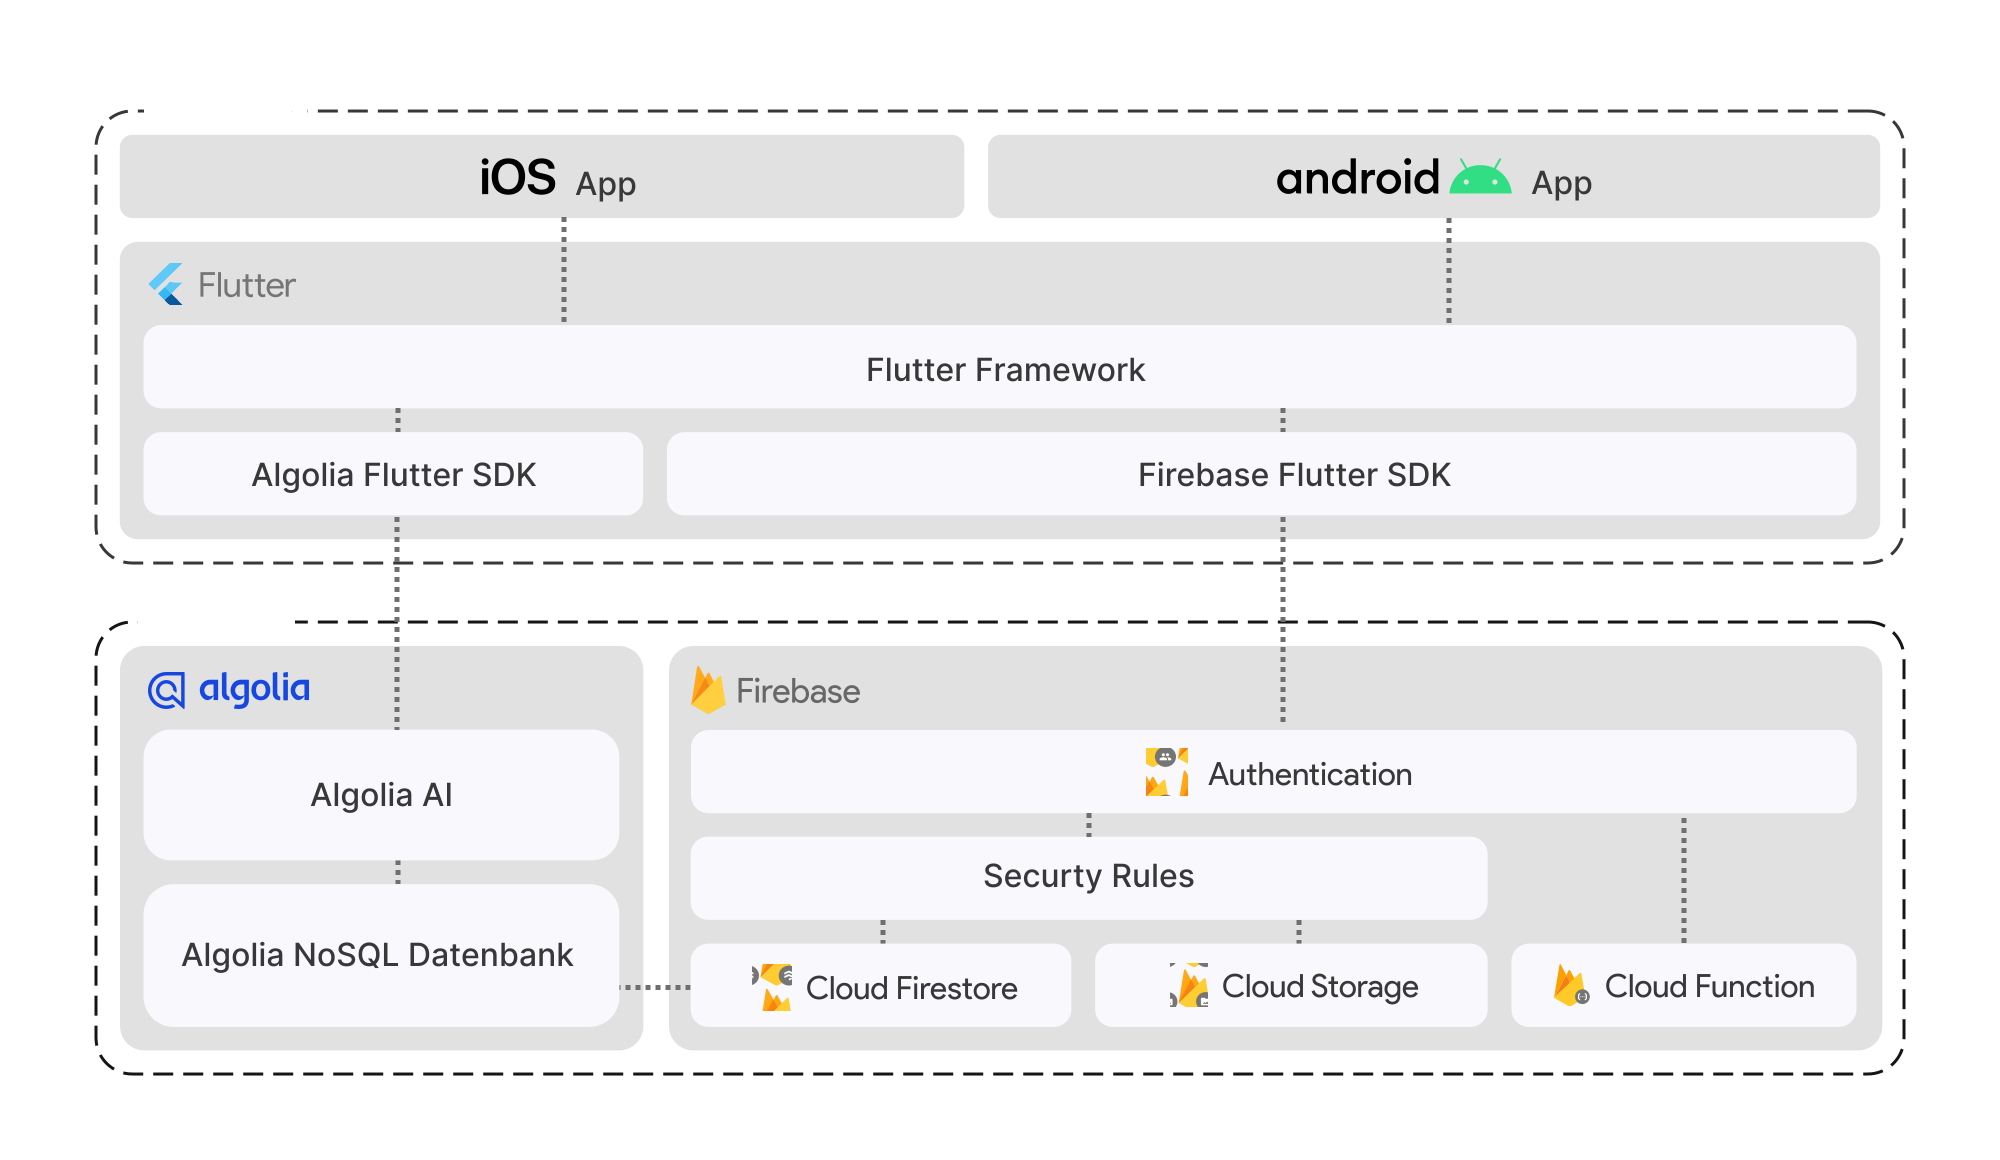
\includegraphics[width=0.2\textwidth]{pics/systemarchitektur_diagram.svg}

\includesvg{pics/systemarchitektur_diagram.svg}


\section{Flutter}

Hier kommt die Beschreibung der Technologie und deren Vorteile/Nachteile, auf Basis von wissenschaftlichen Studien und Erfahrungen aus der Praxis.

Quellen:

https://docs.flutter.dev/resources/architectural-overview

https://flutter.dev/docs/resources/technical-overview,
https://pub.dev/packages/flutter


% \subsection{iOS}
% \subsubsection{CI/CD}

% \subsection{Android}
% \subsubsection{CI/CD}
% \subsubsection{Firebase App Distribution}




\section{Firebase}
\author{Martin Hausleitner}


Hier wird die Vorstellung der Firebase Technologie inklusive deren Funktionen und Vorteile erklärt.

Quellen:

https://firebase.google.com/docs/guides

https://medium.com/flutter-community/flutter-firebase-from-scratch-28c8ba7d98b5

\subsection{Firebase Authentication}

Beschreibung der Firebase Authentication Technologie, inklusive Sicherheitsregeln und Best Practices.

Quellen:

https://firebase.google.com/docs/auth

https://medium.com/flutter-community/firebase-authentication-in-flutter-752d14209a8a

\subsubsection{Security Rules}
\author{Martin Hausleitner}


Hier kommt die Erklärung der Sicherheitsregeln in Firebase Authentication und deren Bedeutung für die App Sicherheit.

Quellen:

https://firebase.google.com/docs/rules

https://firebase.google.com/docs/auth/admin/custom-claims

\subsection{Cloud Firestore}

Vorstellung der Datenbanktechnologie Firestore

Quellen:

https://firebase.google.com/docs/firestore

https://medium.com/flutter-community/firebase-cloud-firestore-in-flutter-26c6e8c6f90c

\subsubsection{Datenmodel}

Hier kommt die Erklärung des Datenmodells in Firebase Firestore und dessen Auswirkungen auf die App-Architektur.

Quellen:

https://firebase.google.com/docs/firestore/data-model

https://www.raywenderlich.com/6628345-cloud-firestore-for-flutter-getting-started

Weitere wichtige punkte:

\begin{compactitem}
    \item Präsentation des eigenen Datenmodells in der Arbeit.
    \item Diagramme werden verwendet, um das Modell zu präsentieren und Entscheidungen zu erläutern und zu begründen.
    \item Anforderungen der App-Architektur werden dabei berücksichtigt werden.
    \item Performance, Skalierbarkeit und Strukturierung können thematisiert werden.
    \item Zur Veranschaulichung unserer eigenen Datenmodell-Entwicklung kann auf ein Beispiel-Datenmodell-Diagramm auf der offiziellen Firebase-Website verwiesen werden, welches uns als Orientierungshilfe diente.
\end{compactitem}

Beispiel-Datenmodell-Diagramm Quelle:

https://firebase.google.com/docs/firestore/data-model\#structure\_your\_data

\subsection{Cloud Storage}

Beschreibung der Cloud Storage Technologie in Firebase und deren Einsatz in der App.

Quellen:

https://firebase.google.com/docs/storage

https://medium.com/flutter-community/firebase-cloud-storage-in-flutter-flutter-an-firebase-tutorial-c5de7835c6cd

\subsection{Firebase Cloud Functions}
\author{Martin Hausleitner}


Erklärung der Cloud Functions Technologie in Firebase, inklusive Beispiele für deren Einsatz in der App.

Quellen:

https://firebase.google.com/docs/functions

https://medium.com/codeburst/organizing-your-firebase-cloud-functions-67dc17b3b0da

\section{Algolia Search}

Vorstellung der Algolia Search Technologie und deren
Integration in die App-Architektur.

Algolia AI

Quellen:

https://www.algolia.com/doc/

https://www.algolia.com/doc/guides/sending-and-managing-data/send-and-update-your-data/tutorials/firebase-algolia/

\subsubsection{Firebase Cloud Function}

Beschreibung der Firebase Cloud Functions und deren Rolle in der Algolia Integration.

Quellen:

https://firebase.google.com/docs/functions

https://www.algolia.com/doc/guides/sending-and-managing-data/send-and-update-your-data/tutorials/firebase-algolia/


\begin{spacing}{1}
	\chapter{Umsetzung}\label{chapter:implementation}
\end{spacing}
\section{Continuous Integration/Delivery}
\subsection{GitHub Actions}

allg. actions warum kosten
\subsubsection{Build IOS}
\author{Martin Hausleitner}

\subsubsection{Build Android}

\subsection{Fastline}
\subsubsection{Build Number increment}
\subsection{Firebase App Distribution}

\section{Mobile Anwendung}
\subsection{Dateistruktur}
\author{Martin Hausleitner}
In Flutter gibt es keine fixe Dateistruktur für eine App,
man kann seine Struktur also selbst überlegen und gestalten.
Im Folgenden beschreibe ich, wie wir unsere Dateistruktur
für eine Flutter-App aufgebaut haben.

In Flutter gibt es keine feste Dateistruktur, stattdessen kann man die Struktur der Dateien und Ordner selbst bestimmen. Für unser Flutter-Projekt haben wir uns für eine Struktur entschieden, die sich an bewährten Praktiken orientiert.

Unsere Dateistruktur sieht wie folgt aus:

\begin{itemize}
    \item \textbf{logic} - Hier befindet sich die Geschäftslogik der App, einschließlich der Firestore-Cloud-Funktionen und Repositories, die API-Aufrufe ausführen.
    \item \textbf{pages} - Hier werden Widgets entworfen, die jeweils eine Seite der App darstellen.
    \item \textbf{routes} - Hier werden die Routen definiert, die tiefere Links ermöglichen.
    \item \textbf{shared} - Hier werden UI-Widgets wie Buttons oder andere Widgets gespeichert, die oft wiederverwendet werden.
    \item \textbf{views} - Hier befinden sich Ansichten, die von mehreren Seiten der App verwendet werden können.
\end{itemize}

Im Nachhinein hätten wir die Dateistruktur anders gestaltet,
z.B. hätten wir das UI als eigenes Package definiert und die
pages und views besser unterteilt.

\subsection{State Management}
In Flutter gibt es verschiedene Möglichkeiten\cite{flutter-docs-interactive}\cite{flutter-state-management-blog}, um mit dem State Management umzugehen. State Management bezieht sich auf die Art und Weise, wie Daten innerhalb einer App verwaltet werden. In jeder App gibt es bestimmte Daten, die von verschiedenen Komponenten und Widgets verwendet werden und sich im Laufe der Zeit ändern können. State Management bezieht sich auf die Methoden, die verwendet werden, um diese Daten innerhalb der App zu verwalten und zu aktualisieren.
\author{Martin Hausleitner}

\subsubsection{GetX}
\author{Martin Hausleitner}

GetX verwendet ein reaktives Ansatz zur Verwaltung des Zustands, was bedeutet, dass Änderungen im Zustand automatisch die UI aktualisieren, ohne dass der Entwickler manuell Code schreiben muss, um diese Aktualisierungen durchzuführen. Dies spart viel Entwicklungszeit und macht es einfach, auf Benutzerinteraktionen zu reagieren.

Mit GetX können wir auch eine einheitliche Datenquelle haben, auf die alle Komponenten zugreifen können, was die Wartung und Erweiterung der Anwendung erleichtert. Darüber hinaus bietet GetX auch eine einfache Möglichkeit, Abhängigkeiten zu verwalten und Zustandsinformationen zwischen Bildschirmen zu teilen.

Insgesamt hat uns die Verwendung von GetX im Flutter-Framework sehr geholfen, eine effektive und skalierbare Anwendung zu erstellen, die auf die Bedürfnisse unserer Benutzer abgestimmt ist.
\author{Sandin Habibovic}
getx controller service etc...


\subsection{Authentifizierung}
\author{Sandin Habibovic}

\subsubsection{Anmelde Flow}
\author{Sandin Habibovic}

Diagram
erklärung
screenshots
\subsubsection{Regestrierungs Flow}
\author{Sandin Habibovic}


Diagram
erklärung
screenshots


\subsubsection{Firebase Authentifizierung}
\author{Sandin Habibovic}

allg.


\subsection{Feed}
\author{Sandin Habibovic}
foto
aufbau

\subsection{Beiträge}
\author{Sandin Habibovic}
Beiträge sind das Hauptkommunikationsmittel auf der App. Jedem Beitrag muss ein Titel, eine Beschreibung und eine Reichweite, unter der, der Beitrag sichtbar ist, angegeben werden. Weiters ist es möglich einem Beitrag ein Bild und Tags anzuhängen.

\subsubsection{Kategorien}
\author{Sandin Habibovic}
Um Beiträge besser zuordnen zu können, muss der User den Beitrag vor dem Veröffentlichen in eine bestimmte Kategorie einteilen. Diese Kategorien ermöglichen es Usern, die Art Ihrer Anfrage ihm vorhinein besser zu spezifizieren und die Suche nach Beiträgen einer bestimmten Art zu vereinfachen. Bestimmte Kategorien werden weiters in Unterkategorien aufgeteilt, da diese ein zu weit gefächertes Genre an Anfragen umfassen.

Es existieren folgende Kategorien bzw. Unterkategorien:

\begin{compactitem}
    \item Mitteilung
    \begin{compactitem}
        \item Frage
        \item Appell
        \item Warnung
        \item Empfehlung
        \item Gefunden
    \end{compactitem}
    \item Suche
    \begin{compactitem}
        \item Hilfe
        \item Verloren
    \end{compactitem}
    \item Ausleihen
    \item Event
\end{compactitem}



Mitteilung:
Die Kategorie der Mitteilung dient dazu die Nachbarn über ein bestimmtes Ereignis oder Meldung zu informieren oder zu befragen.

Suche:
Die Kategorie der Suche dient dazu mit den Nachbarn im Falle einer Hilfesuche oder eines verloren gegangenen Objekts in Kontakt zu treten.

Ausleihen:
Die Kategorie des Ausleihens dient dazu die Nachbarn nach der Erlaubnis, sich ein bestimmtes Werkzeug oder Objekt ausborgen zu dürfen, zu bitten.

Event:
Die Kategorie des Events dient dazu die Nachbarn auf eine bestimmte Veranstaltung aufmerksam zu machen.


\subsubsection{Tags}
\author{Sandin Habibovic}
Als Tag wird ein Schlüsselwort beschrieben, was man an ein Informationsgut anhängen kann, um es besser beschreiben zu können und/oder besser auffindbar zu machen. In der App werden Tags als eine Erweiterung der Kategorien verwendet, um es Usern zu ermöglichen Ihren Beitrag einem selbstdefinierten Typ zuzuordnen.

\subsubsection{Info}
\author{Sandin Habibovic}
Jeder Beitrag hat eine eigene Sektion, wo wichtige Entscheidungsinformationen angegeben werden, wie der Stadtteil und die ungefähre Entfernung zum gegebenen Nachbarn und das Erstelldatum des Beitrags.

\subsubsection{Kommentare}
\author{Sandin Habibovic}
Die Kommentarfunktion ermöglicht es den Usern unter einem Beitrag Ihre Meinung, Feedback oder sonstiges zu hinterlassen.

\subsubsection{Beitrag oder Kommentar Melden}
\author{Sandin Habibovic}
Um auf unangebrachte Beiträge oder Kommentare schnell reagieren zu können, gibt es die Möglichkeit Beiträge oder Kommentare zu melden. Diese Meldungen werden auf Firestore gespeichert und können dann im Einzelnen überprüft werden. Fürs Melden muss ein Grund ausgewählt und eine genauere Beschreibung angegeben werden.
Gründe fürs Melden eines Beitrags oder Kommentars:

\begin{compactitem}
    \item Unangebrachter Inhalt
    \item Belästigung
    \item Betrug
    \item Spam
    \item Sonstiges
\end{compactitem}

\subsection{Filter}
\author{Sandin Habibovic}
Filtern nach Kategorien
Ordnen nach Likes oder Datum
Absteigend oder aufsteigend sortieren

\subsection{Suche}
\subsection{Typesense}
\subsection{Algolia}
diagram
\subsubsection{Firestore Sync}

\subsubsection{Algolia SDK}


\subsection{Chat}
package genommen warum
\subsubsection{Flyer Package}

\subsection{Profil}
\author{Sandin Habibovic}
Was wird angezeigt?
Name, User Public Info, Posts von User

\subsubsection{Profil Melden}
\author{Sandin Habibovic}

\subsection{Benachrichtigungen}
\author{Sandin Habibovic}
Grund und Funktionsweise von Benachrichtigungen
diagram beschreibung
\subsection{Einstellungen}
\author{Sandin Habibovic}
Email/Passwort ändern, Konto löschen, Sprache einstellen, Benachrichtigungen ein/ausschalten
\subsection{Feedback}
\author{Martin Hausleitner}
feedback feature beschreiben


\section{UI/UX Design}
Das UI/UX-Design einer App ist von entscheidender Bedeutung für den Erfolg der App und die Zufriedenheit der Benutzer. Insbesondere bei einer Social-Media-Nachbarschafts-App ist ein gut durchdachtes UI/UX-Design unerlässlich, um eine positive Benutzererfahrung zu gewährleisten.

Ein gutes UI-Design ist wichtig, um sicherzustellen, dass die Benutzer die App einfach und intuitiv bedienen können. Es sollte eine klare Struktur und Navigation haben, damit die Benutzer schnell zu den gewünschten Funktionen gelangen können. Wenn die Benutzer die App als kompliziert oder verwirrend empfinden, werden sie möglicherweise frustriert und geben die Nutzung der App auf.

Auch ein gutes UX-Design ist wichtig, um sicherzustellen, dass die Benutzer mit der App zufrieden sind. Es sollte eine ansprechende und ansprechende Benutzeroberfläche bieten, die dem Benutzer ein angenehmes Nutzungserlebnis vermittelt. Wenn die Benutzer die App als langweilig oder uninteressant empfinden, werden sie möglicherweise nicht wiederkommen.

Darüber hinaus sollte das UI/UX-Design einer Social-Media-Nachbarschafts-App bestimmte Funktionen und Merkmale berücksichtigen, die für eine erfolgreiche Community-Plattform erforderlich sind. Beispielsweise sollte es einfach sein, Beiträge zu erstellen und zu teilen, auf Kommentare zu antworten und Nachrichten an andere Benutzer zu senden. Es sollte auch Möglichkeiten geben, um Benutzerprofile zu erstellen und zu verwalten sowie umfassende Datenschutz- und Sicherheitsfunktionen zu bieten.

Insgesamt ist das UI/UX-Design einer Social-Media-Nachbarschafts-App von entscheidender Bedeutung für den Erfolg der App und die Zufriedenheit der Benutzer. Es ist wichtig, dass das Design auf die Bedürfnisse und Anforderungen der Benutzer zugeschnitten ist und ein einfaches, intuitives und ansprechendes Nutzungserlebnis bietet.
\author{Martin Hausleitner}
\subsection{Inspiration}
Während des Designprozesses für die App habe ich Recherchen im Bereich App-Design durchgeführt. Mein Ziel war es, die App so intuitiv wie möglich zu gestalten, um eine benutzerfreundliche Erfahrung zu gewährleisten. Dazu habe ich mich an bekannten Social-Media-Apps orientiert, wie zum Beispiel Twitter, Instagram und TikTok, die bereits auf dem Markt sehr erfolgreich sind und von vielen Menschen vertraut genutzt werden.

Darüber hinaus hat auch die erfolgreichste Nachbarschafts-App in Deutschland, "Nebenan", viel zur Grundlage der App beigetragen. Allerdings habe ich festgestellt, dass ihre App sehr kompliziert aufgebaut und unübersichtlich ist, was für uns eine Chance darstellte, es besser zu machen.

Zusätzlich haben wir uns von Websites wie Dribble und Mobbin inspirieren lassen, die uns geholfen haben, ein einfaches und schlichtes Design für die App zu entwickeln. Insgesamt war die Recherche und Inspiration für das Design der App ein wichtiger Schritt, um sicherzustellen, dass unsere Benutzer eine ansprechende und intuitive Erfahrung haben.

\subsection{Prototyping}
Prototyping ist ein wichtiger Schritt bei der Entwicklung von mobilen Apps. Es ermöglicht Entwicklern, Designern und anderen Stakeholdern, eine frühzeitige Vorstellung davon zu bekommen, wie die App funktionieren wird und wie sie aussehen wird. Durch die Erstellung eines Prototyps können auch Fehler im Design und in der Funktionalität identifiziert werden, bevor die App in die eigentliche Entwicklung geht.

Es gibt verschiedene Arten von Prototypen, darunter Low-Fidelity- und High-Fidelity-Prototypen. Low-Fidelity-Prototypen sind einfache Skizzen oder Wireframes, die nur die grundlegenden Funktionen und das Layout der App abbilden. High-Fidelity-Prototypen sind detaillierter und können interaktive Funktionen und Designelemente enthalten.

Es gibt viele Tools und Plattformen, die zur Erstellung von Prototypen verwendet werden können. Ein Beispiel ist Adobe XD, das es Entwicklern und Designern ermöglicht, schnelle und einfache Prototypen zu erstellen. Andere Tools wie Sketch, Figma oder InVision sind ebenfalls beliebt.

Der Vorteil von Prototyping ist, dass es Entwicklern und Designern ermöglicht, frühzeitig Feedback von Benutzern zu erhalten und Änderungen vorzunehmen, bevor die App tatsächlich entwickelt wird. Außerdem können Entwickler und Designer Zeit und Ressourcen sparen, indem sie sich auf die richtigen Funktionen und das richtige Design konzentrieren und unnötige Funktionen und Designs vermeiden.

Im Fall von Flutter als Entwicklungsplattform für die App ist das Prototyping ebenfalls wichtig. Flutter bietet verschiedene Widgets und Design-Tools, mit denen Entwickler schnell und einfach Designelemente erstellen und implementieren können. Durch ein gut durchdachtes Prototyping kann Zeit und Aufwand beim Entwickeln gespart werden, da Design-Entscheidungen bereits getroffen wurden und Entwickler sich auf die Umsetzung konzentrieren können.

Insgesamt ist Prototyping ein unverzichtbarer Schritt bei der Entwicklung von mobilen Apps. Es ermöglicht Entwicklern und Designern, frühzeitig Feedback von Benutzern zu erhalten und Änderungen vorzunehmen, bevor die App tatsächlich entwickelt wird. Durch die Verwendung von Tools wie Adobe XD, Sketch oder Figma können Prototypen schnell und einfach erstellt werden, was Zeit und Ressourcen spart. Prototyping ist auch für die Verwendung von Flutter als Entwicklungsplattform wichtig, da es Entwicklern ermöglicht, Zeit und Aufwand zu sparen und sich auf die Umsetzung zu konzentrieren.
\subsubsection{Framer}

Framer ist eine Software, die es Benutzern ermöglicht, schnell und einfach ansprechende Prototypen von mobilen Anwendungen und Websites zu erstellen. Das Tool wurde ursprünglich als Prototyping-Tool für Designer entwickelt, um Designs schnell zu testen und zu verfeinern, bevor sie in die Entwicklung übergehen.

Erfolgreiche Apps wie Spotify haben Framer im Rahmen ihres
Prototyping-Prozesses verwendet, um schnell und effizient
funktionierende App-Designs zu erstellen. Framer ist eine
schnelle und effiziente Möglichkeit, um Ideen in die Tat
umzusetzen, ohne sich durch langwierige Entwicklungsprozesse
zu quälen.

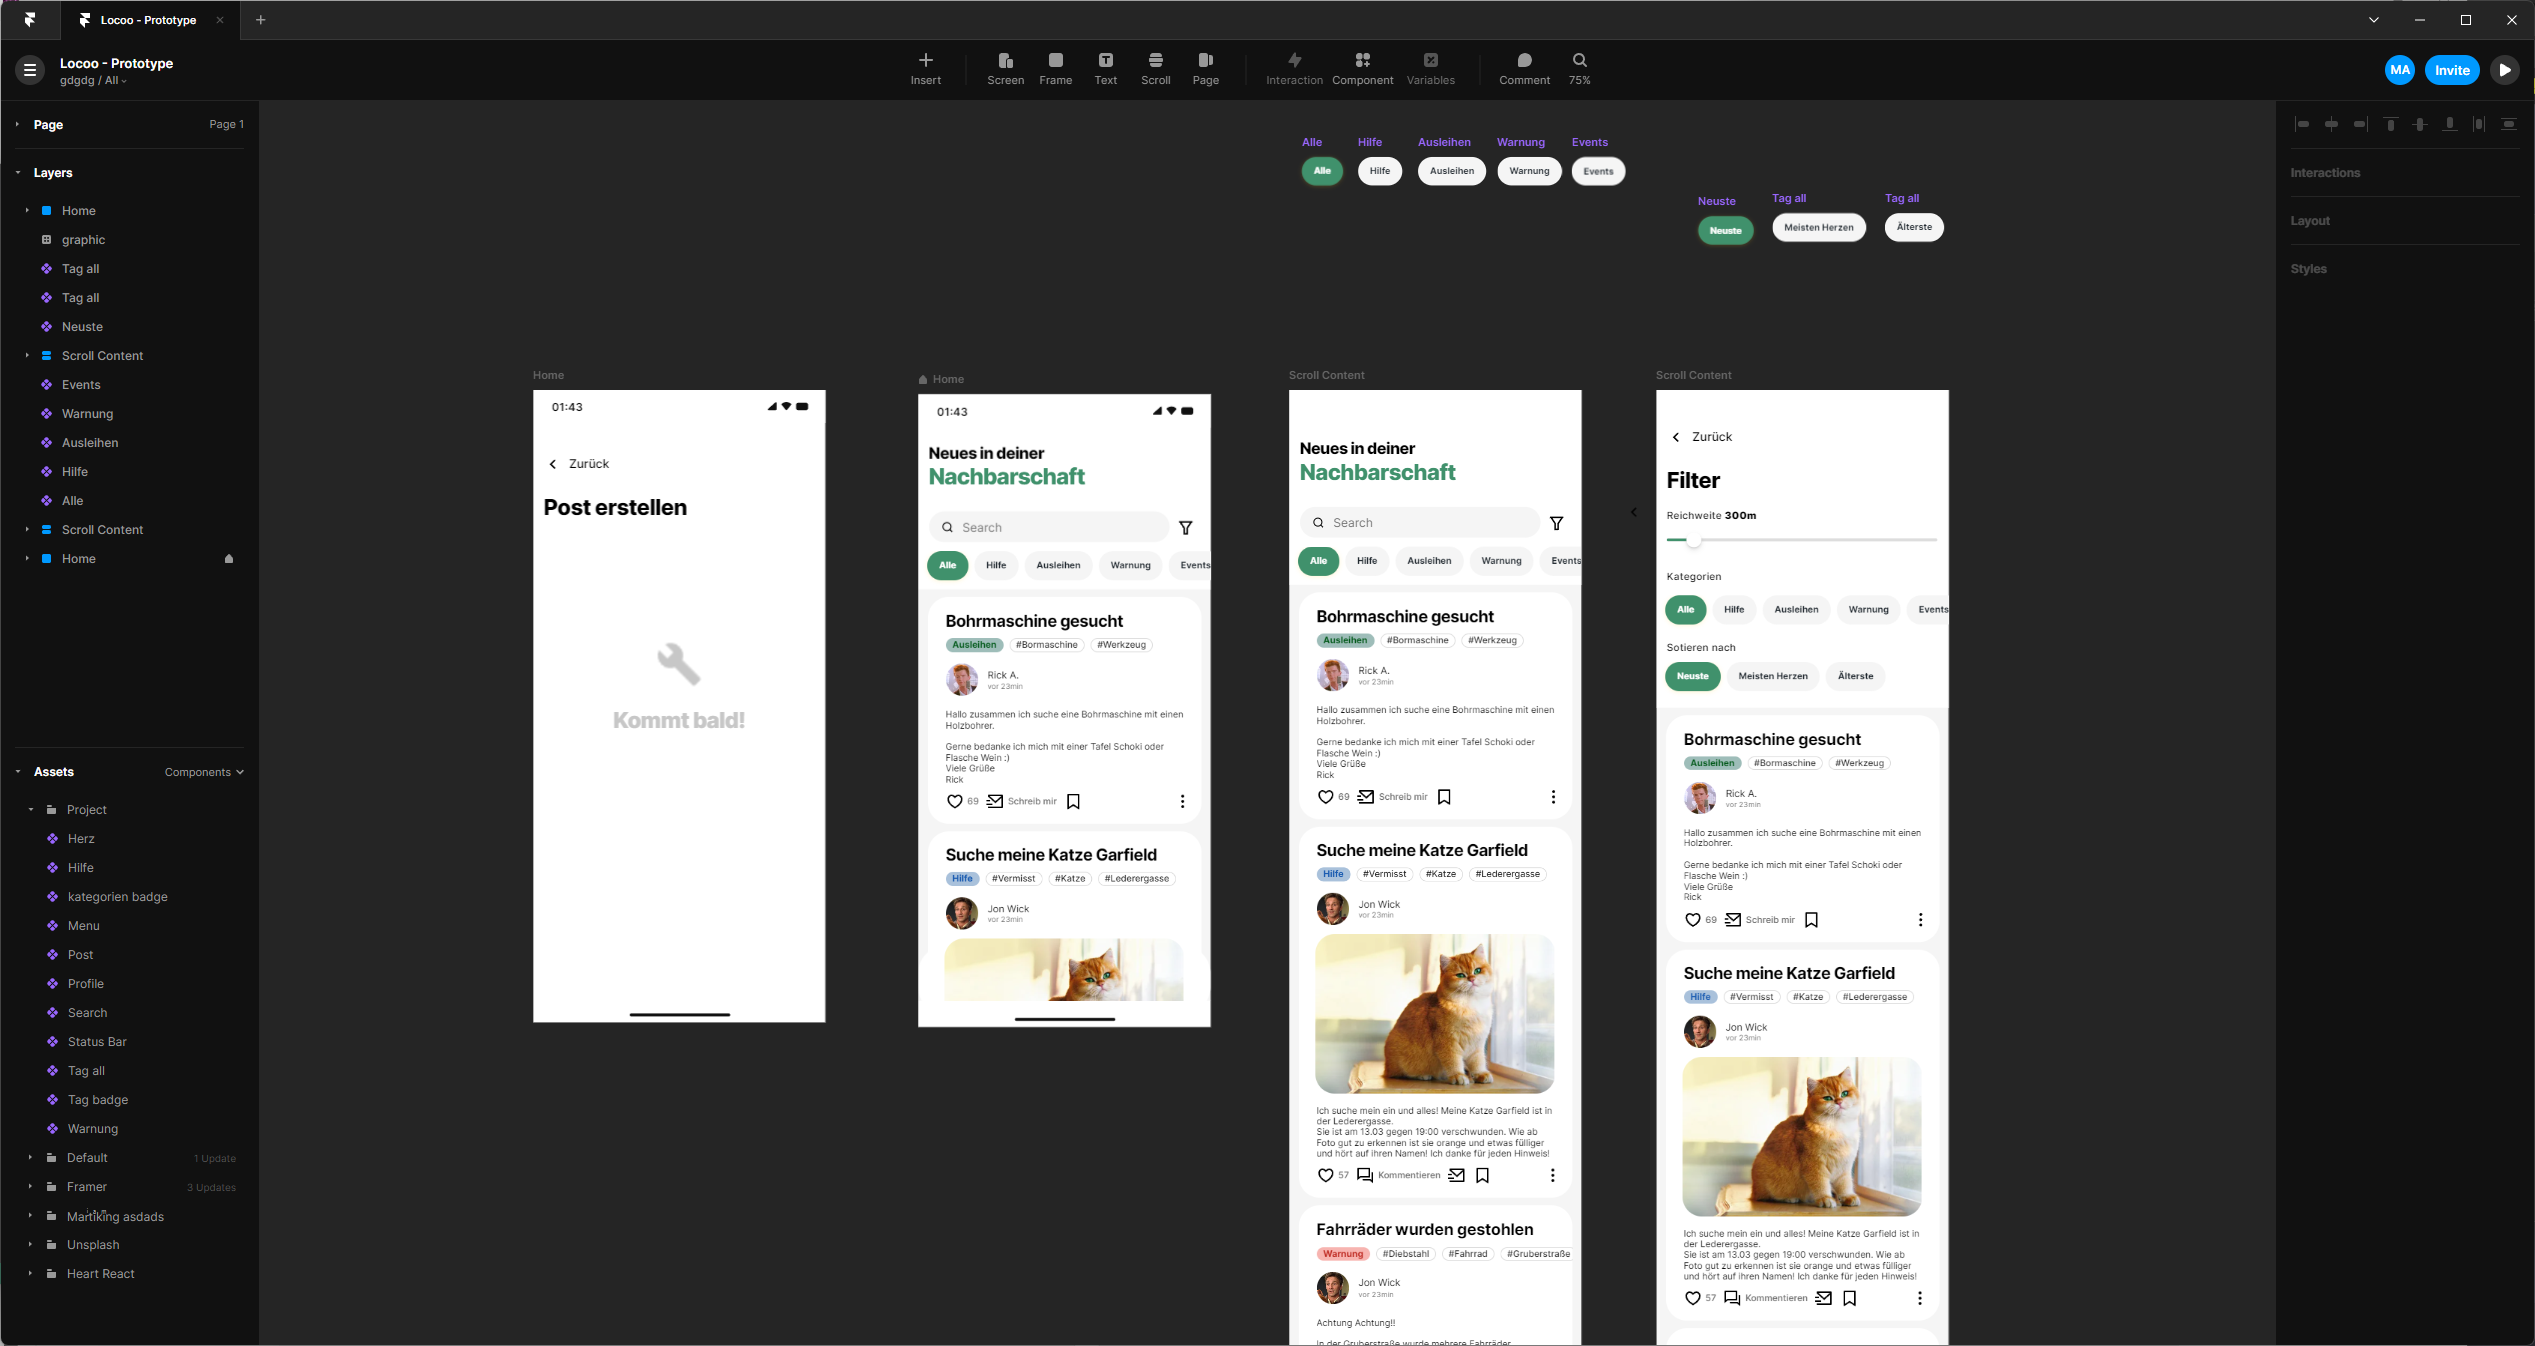
\includegraphics[width=1\textwidth]{pics/nochba-framer-prototype-screenshot.png}


Framer wurde während des Hackerthon Linz hackt verwendet, um den ersten Prototypen zu erstellen. Die Wahl von Framer war aufgrund seiner Geschwindigkeit und Effizienz in der Erstellung von funktionsfähigen App-Designs und der Erfahrung, die der Benutzer bereits mit dem Tool hatte, getroffen worden.

Seit der Erstellung des ersten Prototyps hat sich das Geschäftsmodell von Framer jedoch geändert. Es ist jetzt ein Website-Baukasten, der es Benutzern ermöglicht, einfach und schnell ansprechende Websites zu erstellen, ohne Kenntnisse in der Webentwicklung zu benötigen. Obwohl es nun als Website-Baukasten fungiert, behält Framer immer noch einige seiner Kernfunktionen als Prototyping-Tool bei, was es zu einer guten Option für Designer und Entwickler macht, die schnell Prototypen erstellen möchten.

Insgesamt hat Framer gezeigt, dass es ein schnelles und effektives Tool ist, um Designideen in die Tat umzusetzen. Obwohl es nun als Website-Baukasten fungiert, ist es immer noch eine nützliche Option für Designer und Entwickler, die schnell und einfach Prototypen erstellen möchten.

\subsubsection{Adobe XD}
Als ich zum ersten Mal mit Framer arbeitete, war ich begeistert von den vielen Features und Möglichkeiten, die es bietet. Aber im Laufe der Zeit stellte ich fest, dass es für mein Projekt zu aufwändig war und ich nach einer einfacheren Lösung suchte. So bin ich auf Adobe XD umgestiegen, ein Tool, mit dem ich schon jahrelange Erfahrung hatte.

Obwohl Adobe XD nicht so viele Features wie Framer bietet,
ist es aufgrund seiner Einfachheit und
Benutzerfreundlichkeit ein ideales Tool, um schnell einen
Prototypen zu erstellen. Ich hatte alle Hauptscreens
fertig gestaltet, bevor wir mit der Entwicklung mit Flutter
begannen. Die anderen wichtigen Screens habe ich dann
später gestaltet, als ich mit Flutter vertrauter war und
besser abschätzen konnte, wie aufwändig es in Flutter
umzusetzen war.

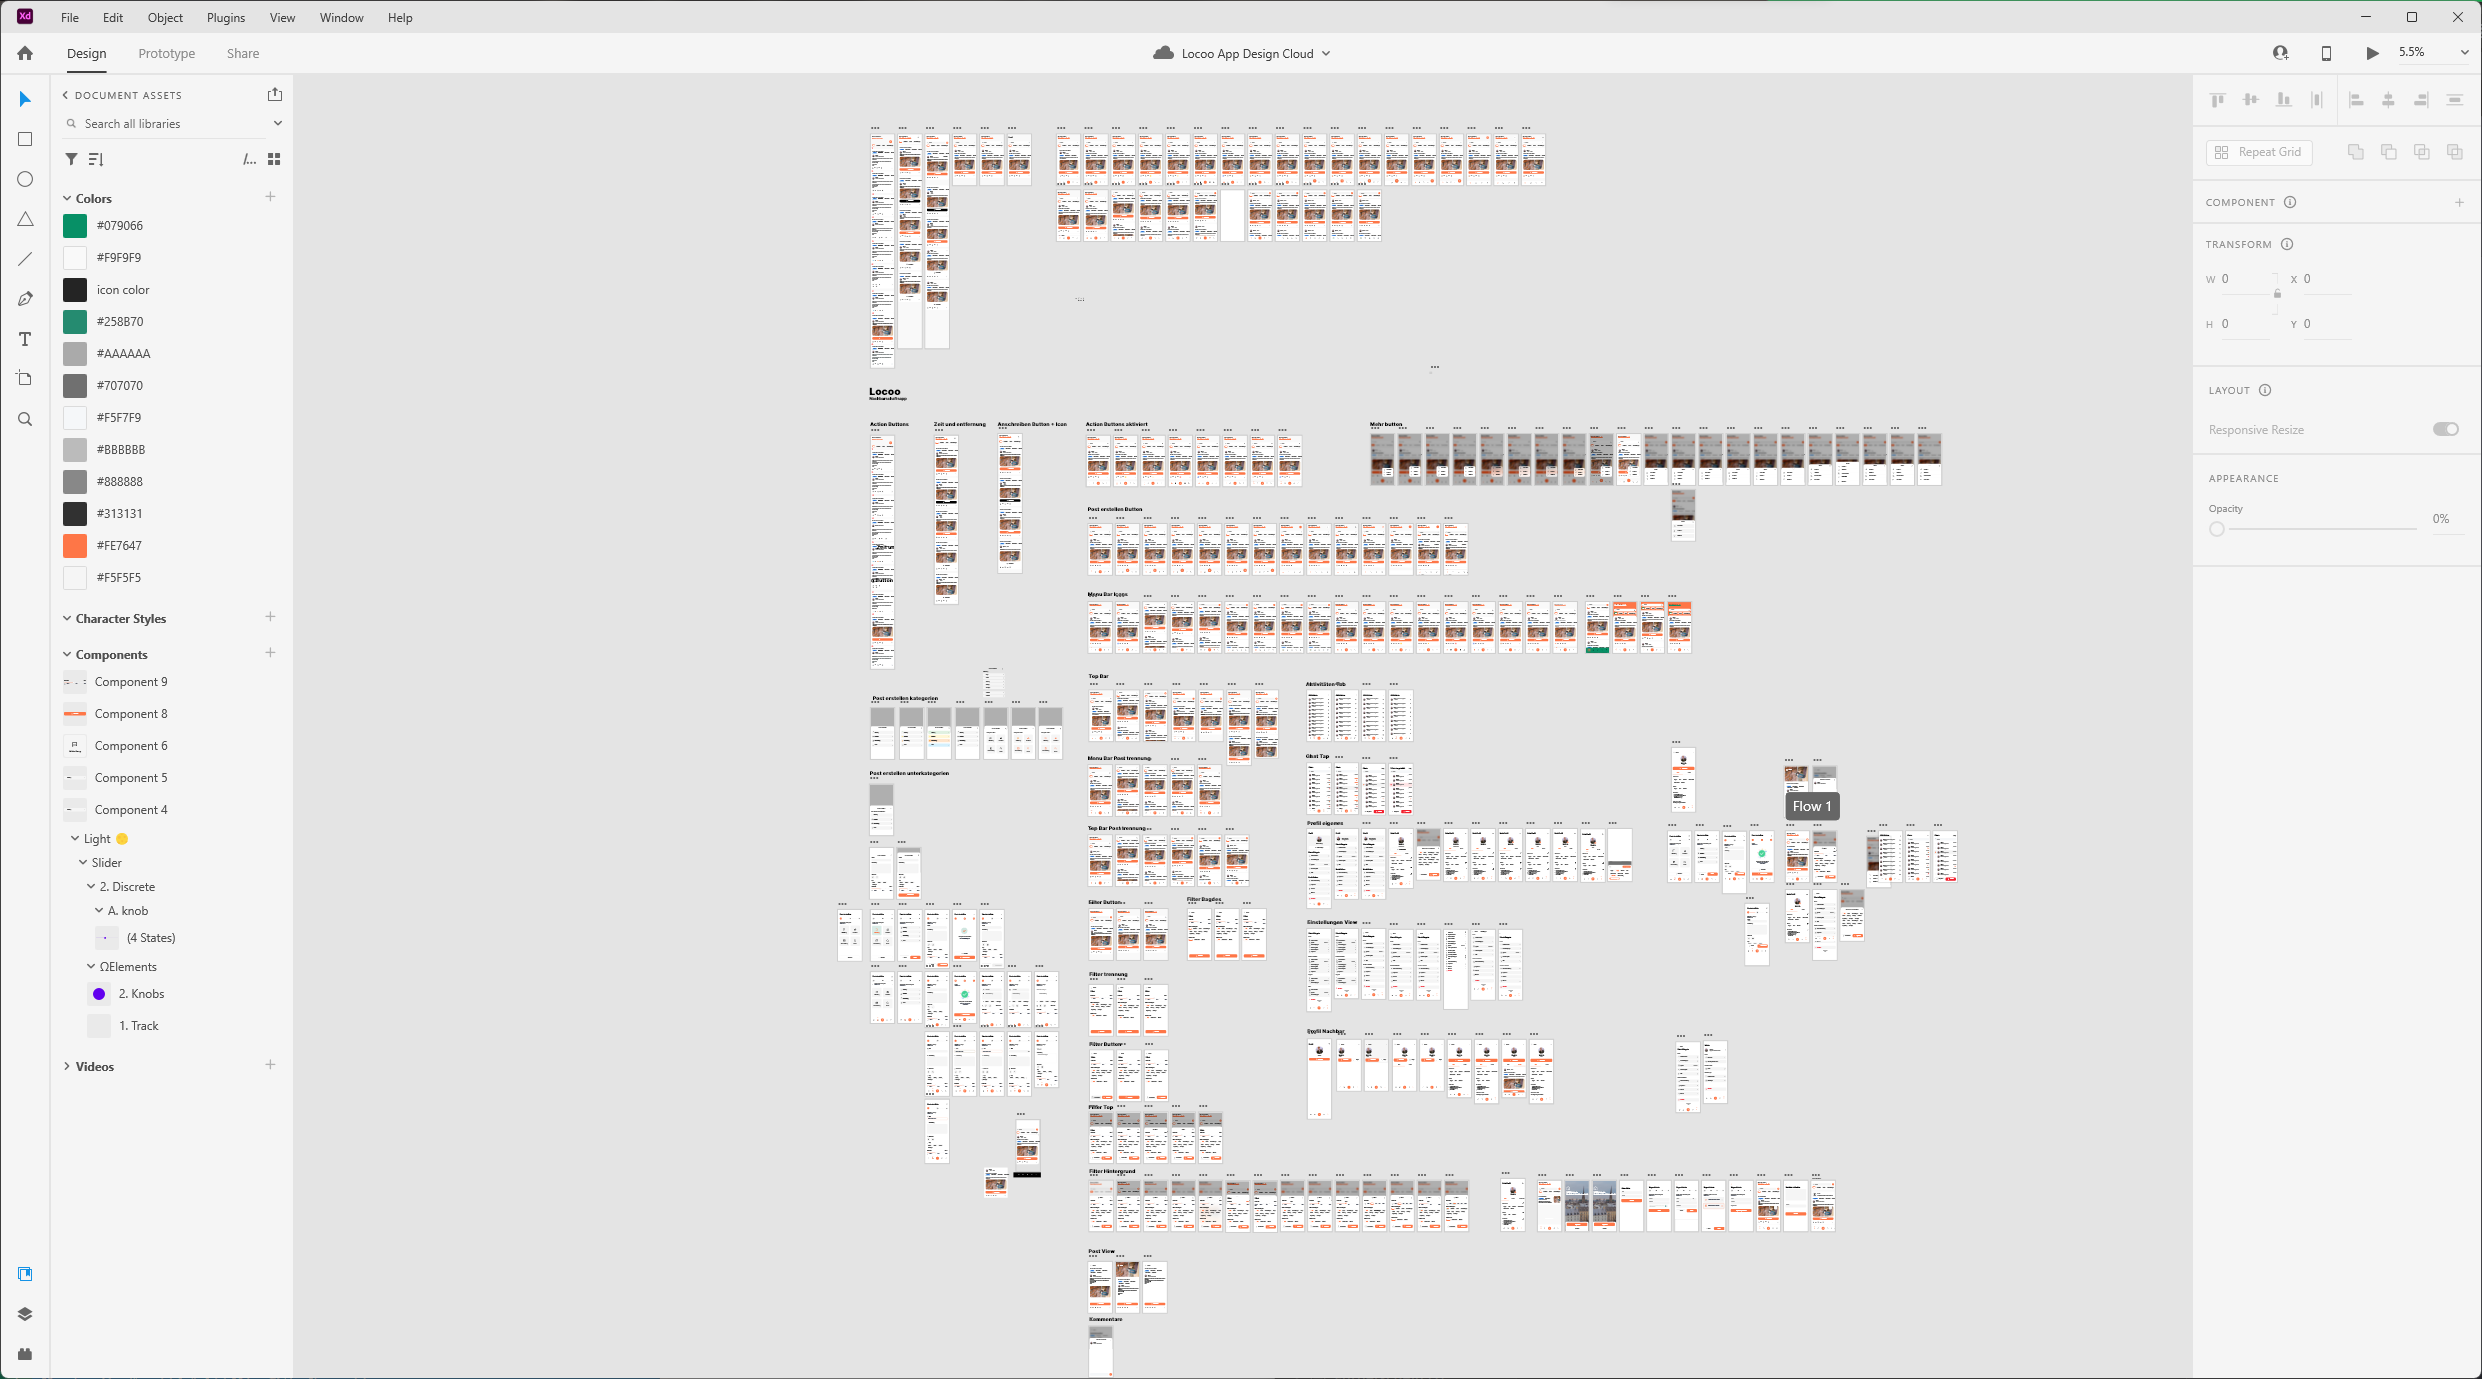
\includegraphics[width=0.95\textwidth]{pics/nochba-adobe-xd-protoype-screenshot.png}


Wie man auf dem obigen Bild sehen kann, ist unser Prototyp
eine Sammlung verschiedener Designs und Evolutionen des
Designs. Adobe XD war für unser Projekt perfekt, da ich der
alleinige Designer war und somit keine
Kollaborationsfunktion benötigte. Allerdings, da ich jetzt
mit dem bekanntesten Designtool Figma vertraut bin und es billiger ist, wenn mehrere
Personen an einem Design arbeiten und auch mehr Funktionen
bietet, würde ich aktuell mit Figma weiterarbeiten.

Zusammenfassend lässt sich sagen, dass Adobe XD ein mächtiges Tool für UI/UX-Designer ist, das einfach zu bedienen und ideal für kleine bis mittelgroße Projekte ist. Es bietet zwar nicht so viele Funktionen wie andere Tools, ist aber für schnelle Prototypenerstellung und einfache Zusammenarbeit mit Entwicklern und Stakeholdern sehr gut geeignet.

\subsection{Design}
allg.


\subsubsection{Farben}
farben history
warum orange
\subsubsection{Icons}

\includegraphics[width=1\textwidth]{pics/icons.png}
In der Abbildung oben sind alle verwendeten Icons in unserer App zu sehen. Es war uns ein wichtiges Anliegen, die App mit so vielen Icons wie möglich auszustatten, um die Bedienung intuitiver und benutzerfreundlicher zu gestalten. Nachdem wir uns mehrere Icon-Packs angesehen hatten, haben wir uns hauptsächlich für die frei verfügbaren Remixicons entschieden. Uns war wichtig, ein eher unbekanntes Icon-Pack zu verwenden, um unsere App von anderen abzuheben und ihr ein einzigartiges Aussehen zu geben. Besonders das verspielte, runde Design hat uns gut gefallen. Ein weiterer großer Vorteil von Remixicons ist, dass es ein Flutter-Paket gibt, was die Implementierung in Flutter vereinfacht hat.

Obwohl Remixicons über 2.271 Icons verfügt, haben uns bei einigen Icons die Material Icons von Google besser gefallen. Daher haben wir einige Icons von Google Material Icons verwendet, insbesondere die abgerundeten Icons, um das Design insgesamt nicht zu hart erscheinen zu lassen. Als ich kein passendes Icon finden konnte, um den Abstand zwischen zwei Nachbarn zu symbolisieren, habe ich mich selbst daran gesetzt, ein passendes Icon im Stil der anderen zu entwerfen.
\subsubsection{Fonts}
fotos von fonts
welche fonts
wie ist due typrographie aufgebaut
\subsubsection{Logo}


\includegraphics[width=0.95\textwidth]{pics/final-logo.png}

% 
\includegraphics[width=0.35\textwidth]{pics/app-logo.png}

% überschrift logo historie
\paragraph{Logo Historie}



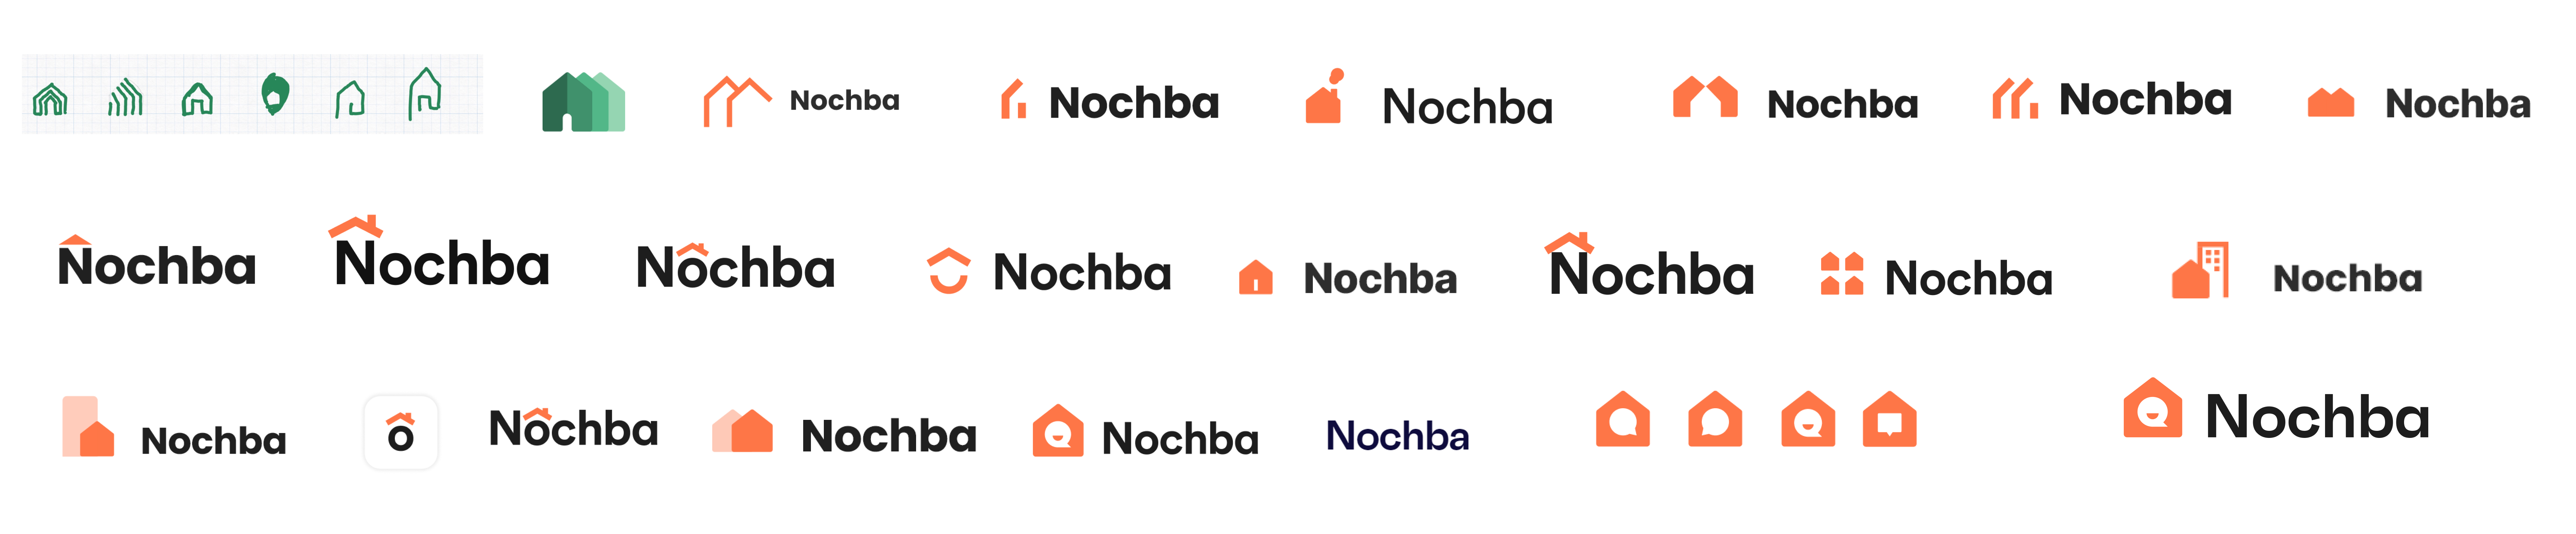
\includegraphics[width=0.95\textwidth]{pics/logo-historie.png}



Im Zuge des Designprozesses haben wir hohe Ansprüche an das
Logo unserer App gestellt, da das logo unser Projekt repräsentiert. Es war uns wichtig, dass es einfach gehalten
und leicht erkennbar ist. Wir haben uns Zeit gelassen, um
den endgültigen Entwurf des Logos zu finalisieren, da uns
die vorherigen Entwürfe nicht vollständig zufrieden
stellten. Ich habe gezielt nach anderen Logos gesucht, die
eine Verbindung zu Nachbarschaften oder Häusern herstellen
und Ideen auf unserem Discord-Server gespeichert. Es sollte
immer ein Haus erkennbar sein, da Häuser schnell mit
Nachbarschaften in Verbindung gebracht werden.

In den früheren Versionen der App hatte ich Schwierigkeiten, ein ansprechendes App-Icon zu gestalten, da ich kein eigenständiges Icon hatte. Aus diesem Grund habe ich mich dazu entschlossen, den Schriftzug und das App-Icon (Logo) separat zu gestalten, wie es auch bei anderen Apps üblich ist. Das endgültige Logo habe ich dann erst Ende 2022 entworfen, da mir alle anderen Designs nicht gefielen. Es ist ein Haus mit einer sprechenden Sprechblase, die lächelt, geworden. Dies soll symbolisieren, dass man innerhalb des Hauses sprechen kann und das Lächeln soll verdeutlichen, dass man Freude mit seinen Nachbarn teilen kann. Generell hat ein Lächeln immer eine positive Wirkung auf den Betrachter und es verdeutlicht, dass es sich bei unserer App um eine Anwendung für den Austausch unter Menschen handelt.

Wir haben bewusst eine runde, verspieltere Schriftart gewählt, da sie besser mit der Farbmischung harmoniert als die vorherige Schriftart.
\subsection{App Design}
\subsubsection{Thumb Zone Prinzip}
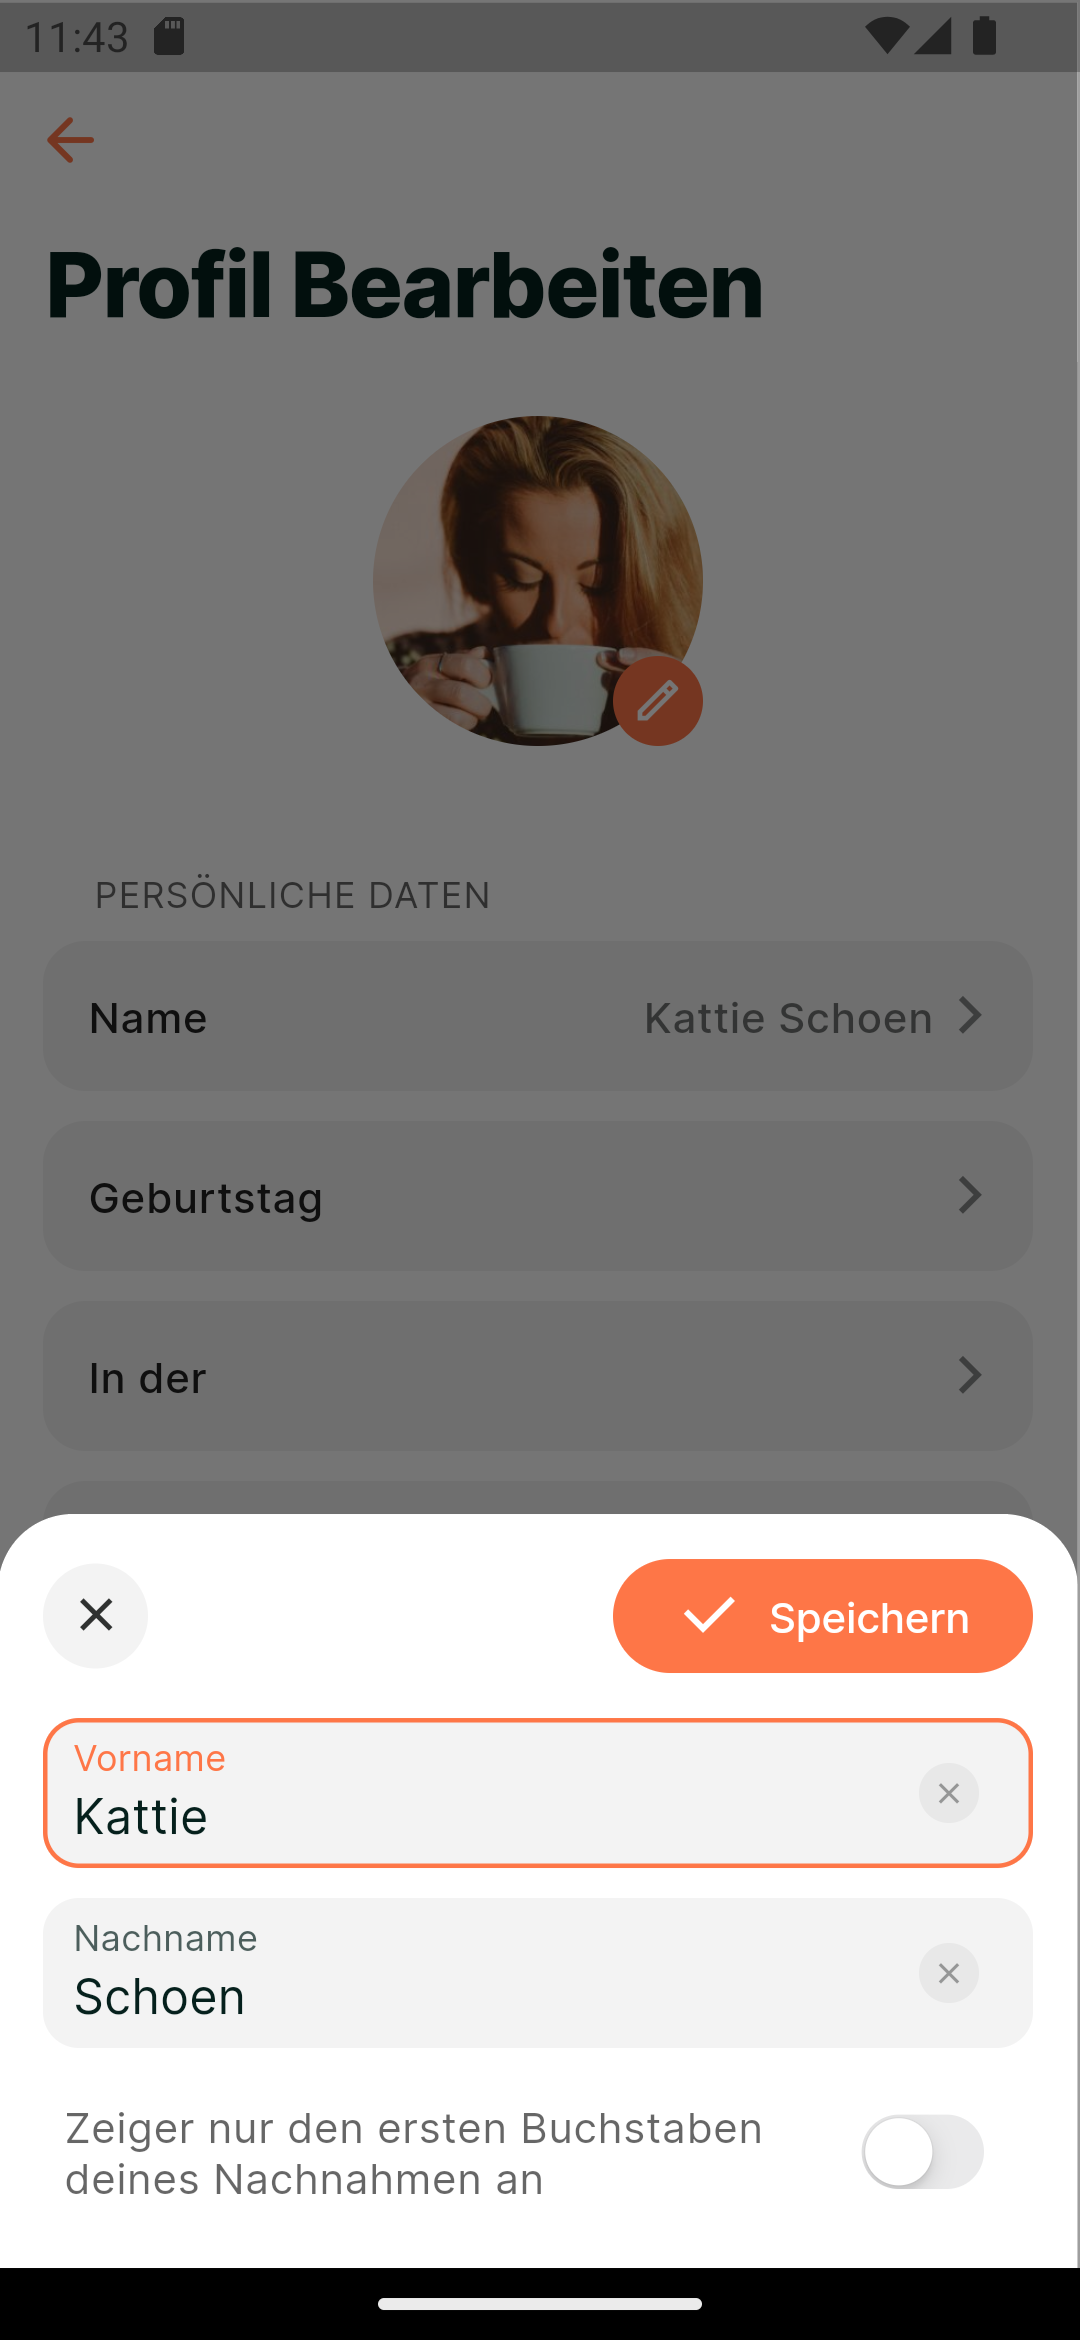
\includegraphics[width=0.3\textwidth]{pics/edit-name-screen.png}
Wir haben versucht, das Thumb Zone Prinzip in unserem Design-Muster zu implementieren, indem wir wichtige UI-Elemente immer im unteren Bereich der App platziert haben. Wenn man die Abbildung betrachtet, kann man deutlich erkennen, dass wir das Layout für die Namensbearbeitung extra unten platziert haben, um alle Klick-Elemente bequem mit dem Daumen bedienen zu können. Wir haben auch alle wichtigen Buttons wie "Speichern" in unserer primären Farbe gestaltet und rechts ausgerichtet, um einen leichteren Zugriff zu gewährleisten. Außerdem haben wir es bei unserer App so implementiert, dass man das Textfeld nicht durch Klicken ändern muss, sondern einfach die Enter-Taste auf der Tastatur drücken kann, um das Eintippen von Daten zu erleichtern. Unwichtige Buttons haben wir in grau gestaltet, wie z.B. den X-Button in der Abbildung. Ein kleines, aber nützliches Feature, das wir eingebaut haben, ist der Löschen-Button neben dem Textfeld, der es dem Benutzer ermöglicht, den gesamten Text bequem zu löschen. Leider ist uns gegen Ende die Zeit ausgegangen, um diese Prinzipien vollständig umzusetzen. In zukünftigen Versionen der App möchten wir sicherstellen, dass diese Prinzipien einheitlich angewendet werden.
\subsubsection{Design Historie}

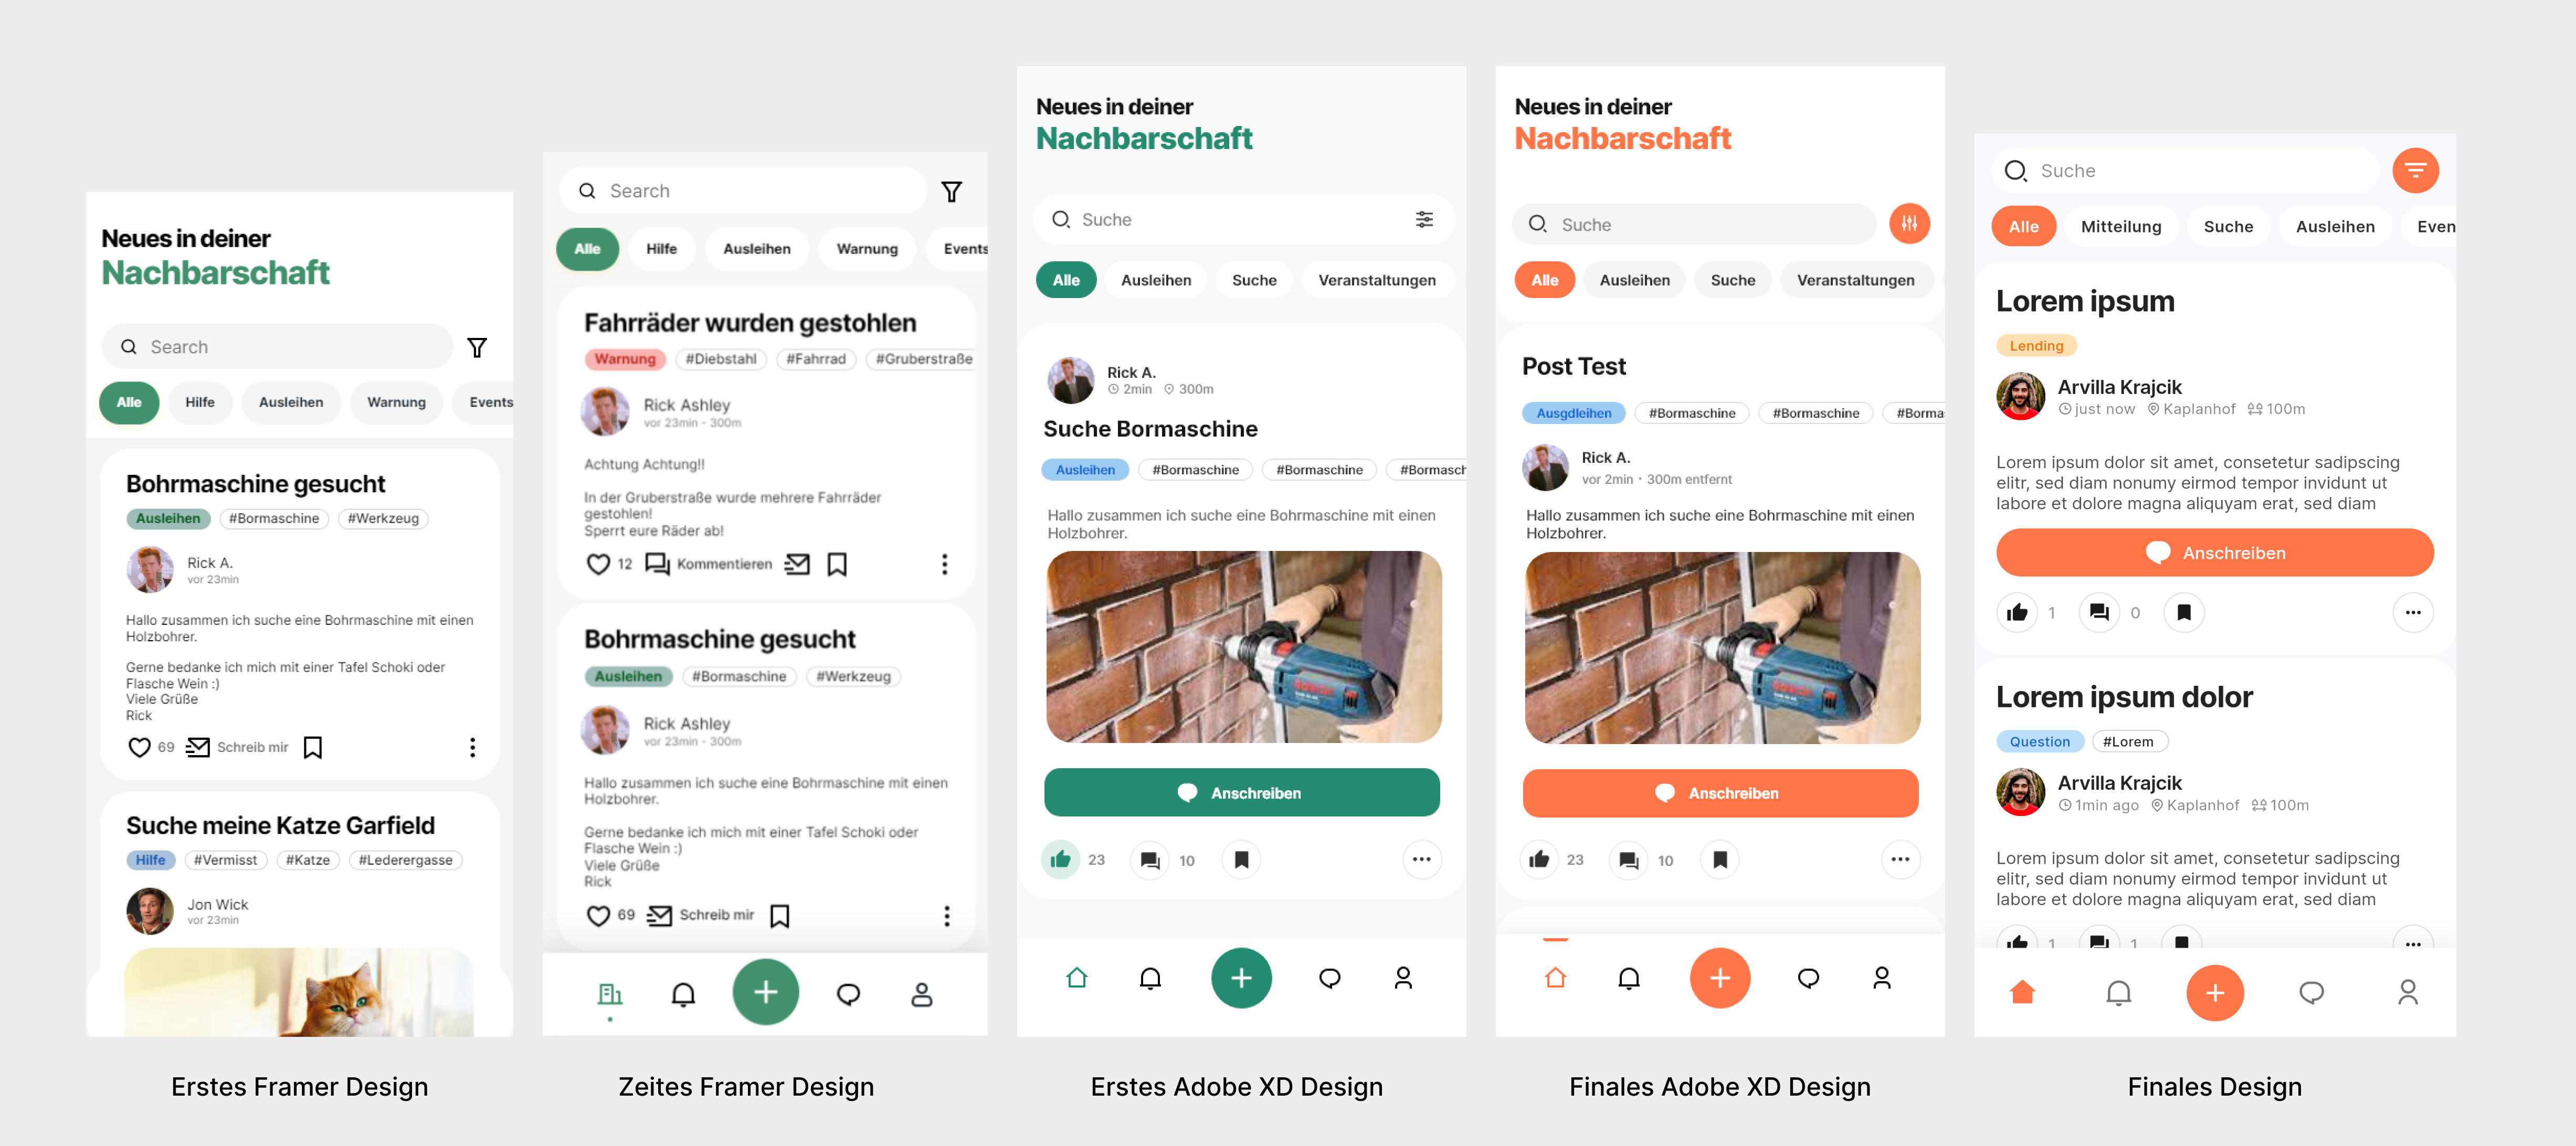
\includegraphics[width=0.95\textwidth]{pics/app-design-history.png}

eingehen mit fotos und beschreibung auf die haupt screens der app

\subsection{Websiten Design}

\includegraphics[width=1\textwidth]{pics/website-design.png}


Da unser Projekt aufgrund unserer Teilnahme an Linz hackt in den Medien präsent war und wir keinen zentralen Anlaufpunkt für Informationen hatten, haben wir uns entschlossen, eine schlichte Landing Page mit grundlegenden Informationen zu gestalten. Das wichtigste Feature unserer Website ist die Möglichkeit für Nutzer, sich für die Testphase zu registrieren. Bei der Gestaltung der Landing Page ließ ich mich von den Vorlagen von Framer inspirieren und nutzte hauptsächlich fertige Abschnitte. Wir hielten uns an unsere Farbpalette und achteten darauf, dass die Webseite möglichst einfach gestaltet ist. Ursprünglich hatten wir nicht geplant, eine Website für unser Projekt zu erstellen.

\section{Backend}

\subsection{Firebase}
\author{Martin Hausleitner}
Firebase ist ein BaaS, das uns Entwicklern eine erhebliche Menge an Stress abnimmt. Das Hosting von Datenbanken oder in unserem Fall Cloud-Funktionen funktioniert mit nur wenigen Klicks. Wir müssen uns keine Gedanken über Skalierung oder Ausfälle machen. Unser Firebase-Backend hosten wir auf der Google Cloud in Frankfurt (EUR3 Europe-West), um eine geringe Latenz zu gewährleisten. Zu Beginn haben wir den kostenlosen Plan "Spark" genutzt, was für uns ausreichend war, da wir noch nicht die Firebase-Cloud-Funktionen genutzt haben. Um Geld zu sparen, haben wir dann lange Zeit mit dem lokalen Firebase-Emulator an den Cloud-Funktionen gearbeitet. Im Januar 2023 sind wir dann auf den "Blaze"-Plan umgestiegen, um die Firebase-Cloud-Funktionen nutzen zu können. Bis zum Stand März 2022 haben wir nur wenige Euro für den Verbrauch gezahlt. Wir waren auch sehr beeindruckt von der exzellenten Dokumentation und den vielen Tutorials auf YouTube, die Firebase anbietet.


\subsection{Firebase SDKs}
\author{Sandin Habibovic}
Firebase-Tools

\subsection{Firebase Authentication}
\author{Sandin Habibovic}
Email und Passwort authentication

\subsection{Cloud Firestore}
\author{Sandin Habibovic}
NoSQL-Database, Dokument-basierte Speicherung, Subcollections
\subsection{Cloud Storage}
\author{Sandin Habibovic}
Speicherung von Profilbilder und Post-Bilder
\subsection{Firebase Cloud Functions}
\author{Martin Hausleitner}
Firebase Cloud Functions sind eine großartige Möglichkeit,
um Business-Logik abzubilden. Es handelt sich um serverlose
Funktionen, die in JavaScript oder TypeScript geschrieben
werden und einzeln auf der Google Cloud gehostet werden. Je
nach Nachfrage werden sie automatisch skaliert oder komplett
abgeschaltet. Ein Nachteil ist, dass die Startup-Zeit länger
sein kann als bei einem herkömmlichen Backend, das immer
läuft. Allerdings kann man durch Cloud Functions viel Geld
sparen, da nur die Prozessorlaufzeit bezahlt werden muss.

Firebase Cloud Functions ermöglichen es Entwicklern, auf verschiedene Ereignisse in Firebase-Produkten zu reagieren. Zum Beispiel, wenn sich Daten in der Firestore-Datenbank ändern oder ein neuer Nutzer in Firebase Authentication registriert wird. Wenn ein solches Ereignis eintritt, wird die entsprechende Cloud Function automatisch ausgeführt.

Wir haben alle Cloud Functions in TypeScript programmiert,
da TypeScript Typsicherheit und erweiterte Fehlererkennung
bietet.


\subsubsection{Regestrierung mit einen Verifizierungscode}
\author{Martin Hausleitner}

Die Cloud-Funktion "checkVerificationCode" wird ausgeführt, wenn ein Nutzer sich mit einem Verifizierungscode registrieren möchte Wenn der Benutzer nicht authentifiziert ist, wird eine HttpsError ausgelöst. Dann wird der Verifizierungscode überprüft, um sicherzustellen, dass er die korrekte Formatierung hat. Wenn der Code ungültig ist, wird eine weitere HttpsError ausgelöst.

Als Nächstes wird der Verifizierungscode mit der Datenbank
abgeglichen, um sicherzustellen, dass er aktiv und noch
nicht zu oft verwendet wurde. Wenn der Code erfolgreich
validiert wird, wird die Adresse des Benutzers abgerufen und
deren Koordinaten mithilfe von einer API call
anOpenStreetMap mit der Funktion "getOSMCoordinatesFromAddress"
ermittelt. Dann wird die Entfernung zwischen der Adresse des
Benutzers und der Adresse, die dem Verifizierungscode
zugeordnet ist, berechnet mit der Funktion "getDistanceFromLatLonInMeters". Wenn die Entfernung nicht
innerhalb des zulässigen Bereichs liegt, wird eine weitere
HttpsError ausgelöst.

Schließlich werden die Informationen des Benutzers und des
Verifizierungscodes in der Datenbank aktualisiert, um
anzuzeigen, dass der Benutzer erfolgreich verifiziert wurde.
Die Cloud-Function gibt true zurück, um anzuzeigen, dass die
Verifizierung erfolgreich war.

In jeder Phase der Funktion wird ein Logger verwendet, um Informationen über den Status der Funktion zu protokollieren.

\subsubsection{Regestrierung mit Gerät Koordinaten}
\author{Martin Hausleitner}

Die Cloud-Funktion "checkAddressWithDeviceLocation" erfordert eine authentifizierte Anfrage und
erhält eine Adresse, eine Längen- und Breitengradkoordinate
vom Gerät des Benutzers. Die Funktion prüft, ob alle
erforderlichen Daten vorhanden sind und ruft dann die
Funktion "getOSMCoordinatesFromAddress" auf, um die
Koordinaten der angegebenen Adresse zu erhalten. Es wird
auch die Funktion "getDistanceFromLatLonInMeters"
aufgerufen, um die Entfernung zwischen der Adresse und den
Koordinaten des Geräts des Benutzers zu berechnen.

Wenn die Entfernung größer ist als ein vordefinierter maximaler Abstand, wird eine Fehlermeldung ausgegeben und die Funktion gibt "false" zurück. Andernfalls speichert die Funktion die Koordinaten der Adresse und die Entfernung zwischen den Koordinaten des Geräts des Benutzers und der Adresse in der Firestore-Datenbank. Die Funktion ruft auch die Funktion "getOSMSuburbFromCoords" auf, um den Vorort der Adresse zu erhalten, und speichert diesen ebenfalls in der Firestore-Datenbank.

Die Funktion gibt "true" zurück, wenn die Verifizierung
erfolgreich abgeschlossen ist.

In jeder Phase der Funktion wird ein Logger verwendet, um Informationen über den Status der Funktion zu protokollieren.

\subsubsection{Verifizierungscode generieren}
\author{Martin Hausleitner}
Die Cloud-Funktion "generateVerificationCode" definiert Konstanten
für das Intervall zwischen der Generierung von Codes, die
maximale Anzahl von Codes und die Reichweite in Metern.

Anschließend wird der letzte code des nutzers aus der
Datenbank geholt, um zu überprüfen, ob seit dem
letzten generierten Code ausreichend Zeit vergangen ist.
Wenn ja, wird der zuletzt generierte Code zurückgegeben.

Wenn nicht, wird eine Schleife gestartet, um einen neuen
Code zu generieren mit der Funktion "generateRandomVerificationCode". Der generierte Code wird dann mit
Firestore abgeglichen, um sicherzustellen, dass er nicht
bereits verwendet wurde.

Wenn der generierte Code eindeutig ist, wird überprüft ob
der Benutzer verifiziert ist. Wenn dies nicht der Fall ist,
wird ein Fehler zurückgegeben. Andernfalls wird der
generierte Code in die
Firestore-Datenbank eingefügt um den letzten generierten
Code und das Datum der Generierung zu speichern.

Das Skript gibt dann den generierten Code zurück. In jeder
Phase der Funktion wird ein Logger verwendet, um
Informationen über den Status der Funktion zu
protokollieren.

\subsubsection{Koordienaten von }
\author{Martin Hausleitner}

\subsubsection{Entferung von zwei Nutzern berechnen}
\author{Martin Hausleitner}
Die Cloud-Funktion "getDistanceFromTwoUsers" berechnet die
Entfernung zwischen zwei Benutzern. Die Funktion erwartet
eine PostId und einen Authentifizierten bneutzer. Dann wird eine
Überprüfung durchgeführt, ob der Post mit der angegebenen ID
existiert und ob der Post eine gültige Reichweite hat. Es
werden auch Überprüfungen durchgeführt, ob die
Benutzerkoordinaten vorhanden sind, und ob die Entfernung
zwischen beiden Benutzern innerhalb des Postbereichs liegt.

Die Funktion nutzt die importierten Funktionen
getDistanceFromLatLonInMeters und getNearestDistance, um die
Entfernung in Metern zu berechnen. Allerdings wird die
berechnete Distanz grob gerundet, um die Privatsphäre der
Nutzer zu wahren. Dabei
werden die Längen- und Breitengradkoordinaten von zwei
Benutzern miteinander verglichen, die aus der
Firestore-Datenbank abgerufen werden. Wenn die Entfernung
größer als die Reichweite des Posts ist, wird ein Fehler
ausgegeben.

Schließlich gibt die Funktion die Entfernung zurück.

\subsubsection{Entfernung von zwei geographischen Koordinaten berechnen}
\author{Martin Hausleitner}

\begin{lstlisting}[language=Java,caption=getDistanceFromLatLonInMeters Funktion]
    export function getDistanceFromLatLonInMeters(
        lat1: number,
        lon1: number,
        lat2: number,
        lon2: number
      ) {
        if (lat1 < -90 || lat1 > 90 || lon1 < -180 || lon1 > 180) {
          throw new Error(
            "Invalid coordinate: lat1 must be between -90 and 90, lon1 must be between -180 and 180"
          );
        }
        if (lat2 < -90 || lat2 > 90 || lon2 < -180 || lon2 > 180) {
          throw new Error(
            "Invalid coordinate: lat2 must be between -90 and 90, lon2 must be between -180 and 180"
          );
        }
        const R = 6371; // Radius der Erde in km
        const dLat = deg2rad(lat2 - lat1); // deg2rad unten
        const dLon = deg2rad(lon2 - lon1);
        const a =
          Math.sin(dLat / 2) * Math.sin(dLat / 2) +
          Math.cos(deg2rad(lat1)) *
            Math.cos(deg2rad(lat2)) *
            Math.sin(dLon / 2) *
            Math.sin(dLon / 2);
        const c = 2 * Math.atan2(Math.sqrt(a), Math.sqrt(1 - a));
        const d = R * c * 1000; // Distanz in Metern
      
        if (lat1 === lat2 && lon1 === lon2) return 0;
        return d;
      }
      
      function deg2rad(deg: number) {
        return deg * (Math.PI / 180);
      }
      
\end{lstlisting}
Der vorliegende Code implementiert eine Funktion, die die Distanz in Metern zwischen zwei geographischen Koordinaten (Breitengrad und Längengrad) auf der Erdoberfläche berechnet. Die Funktion verwendet die Haversine-Formel, die auf der Kugelgeometrie basiert, um die kürzeste Entfernung zwischen zwei Punkten auf der Erdoberfläche zu berechnen.

Die Funktion "getDistanceFromLatLonInMeters" hat vier Parameter: "lat1" und "lon1" sind die Breiten- und Längengrade des ersten Punktes, während "lat2" und "lon2" die Breiten- und Längengrade des zweiten Punktes sind, zwischen denen die Distanz berechnet werden soll.

Zu Beginn des Codes werden die Eingabeparameter auf ihre Gültigkeit geprüft und eine Fehlermeldung wird ausgegeben, falls eine der Koordinaten außerhalb des Bereichs von -90 bis 90 für die Breite und -180 bis 180 für die Länge liegt.

Die Funktion berechnet dann die Differenzen der Breiten- und Längengrade sowie den Radius der Erde (R) in Kilometern. Die Differenzen werden dann in Radianten umgewandelt und die Haversine-Formel wird angewendet, um die Entfernung in Kilometern zu berechnen. Schließlich wird das Ergebnis in Meter umgewandelt und zurückgegeben.

Die Funktion "deg2rad" wird als Hilfsfunktion definiert, um Grad in Radianten umzurechnen.

Die Funktion gibt 0 zurück, falls die beiden
Eingabeparameter denselben Wert haben, um zu vermeiden, dass
eine sehr kleine Distanz als Ergebnis ausgegeben wird, wenn
es sich um denselben Punkt handelt.

Quelle: https://www.movable-type.co.uk/scripts/latlong.html

\subsubsection{Bestimmung der nächstgelegenen Entfernung}
\author{Martin Hausleitner}

Um die Privatsphäre der Nachbarn zu gewährleisten, benötigen wir eine Funktion, die uns den nächstgelegenen Abstand zu den Nachbarn gibt, ohne den genauen Abstand preiszugeben. Die Funktion heißt "getNearestDistance" und bekommt einen Meterwert als Parameter.

Die Funktion erstellt ein Array mit den Optionen [100, 200, 500, 1000, 5000, 10000, 15000] und setzt die Variable "nearest" auf den ersten Wert im Array.

Dann wird eine Schleife ausgeführt, die durch jedes Element im Array "options" geht und prüft, welches Element am nächsten zum angegebenen Abstand "distance" liegt. Wenn ein Element näher ist als das bisher am nächsten liegende Element, wird "nearest" aktualisiert.

Schließlich wird überprüft, ob "nearest" größer oder gleich
1000 ist, und je nachdem wird der Abstand entweder in
Kilometern oder Metern zurückgegeben. Wenn der Abstand
größer oder gleich 1000 ist, wird die Einheit "km"
hinzugefügt, ansonsten wird "m" hinzugefügt. Wir haben
absichtlich keine Switches oder If-Bedingungen benutzt, da
wir es jetzt mit der aktuellen Funktion schneller schaffen,
die Abstände zu ändern. Wir evaluieren noch, wie das Array
mit den Optionen aussieht.


\subsubsection{Nachbarschaft von Nutzer bestimmen}
\author{Martin Hausleitner}
Um unseren App-Nutzern ein besseres Verständnis für die Nachbarschaften zu geben, in denen ihre Nachbarn wohnen, zeigen wir bei jedem Benutzer die Nachbarschaft an, in der sie leben. Diese Information wird automatisch in der Datenbank gespeichert, wenn der Nutzer verifiziert wird. Um diese Funktion zu ermöglichen, verwenden wir die folgende Funktion, die die geografischen Koordinaten des Benutzers verwendet, um die entsprechende Nachbarschaft mithilfe der OpenStreetMap-API abzurufen:

Die Funktion heißt "getOSMSuburbFromCoords" und nimmt zwei Parameter entgegen: "lat" für die geografische Breite und "lon" für die geografische Länge des Benutzers. Diese Funktion gibt eine Promise zurück, die eine Zeichenfolge (String) mit dem Namen der Nachbarschaft des Benutzers enthält. Die Funktion verwendet die "axios"-Bibliothek, um eine GET-Anfrage an die OpenStreetMap-API zu senden. Diese Anfrage enthält die geografischen Koordinaten des Benutzers und die gewünschte Zoomstufe (18), um die Nachbarschaft zu finden. Wenn die Anfrage erfolgreich ist, gibt die Funktion den Namen der Nachbarschaft zurück, der aus den Daten extrahiert wird, die von der API zurückgegeben werden. Wenn der Name der Nachbarschaft nicht verfügbar ist, gibt die Funktion den Namen der Stadt oder der Gemeinde zurück, in der sich der Benutzer befindet. Wenn auch diese Informationen nicht verfügbar sind, gibt die Funktion null zurück. Wenn bei der Anfrage ein Fehler auftritt, wird eine Fehlermeldung ausgelöst.

\subsubsection{Verifizierungscode format überprüfen}
\author{Martin Hausleitner}
Um die Laufzeit bei der Verifizierung von Cloud-Funktionen zu optimieren, ist es sinnvoll, am Anfang der Verifizierung eine Überprüfung durchzuführen, ob der Verifizierungscode das richtige Format hat. Dazu wird die Funktion \verb|verifyVerificationCode| genutzt werden, welche einen \verb|string| als Parameter erwartet und einen \verb|Boolean|-Wert zurückgibt. In der Funktion wird ein regulärer Ausdruck (Regex) definiert, um sicherzustellen, dass der Verifizierungscode den Anforderungen entspricht. Der Regex lautet \verb|/^[a-zA-Z0-9]{10}$/|, was bedeutet, dass der Code aus genau 10 alphanumerischen Zeichen bestehen muss. Mit der Methode \verb|test| wird der übergebene Code auf Übereinstimmung mit dem Regex geprüft und das Ergebnis als \verb|Boolean|-Wert zurückgegeben.


\subsubsection{Verifizierungscode generator}
\author{Martin Hausleitner}

Die Funktion \texttt{generateRandomVerificationCode} erzeugt einen zufälligen Code mit einer Länge von 10 Zeichen, indem sie eine Kombination aus Groß- und Kleinbuchstaben des englischen Alphabets sowie Ziffern von 0 bis 9 verwendet. Dabei wird \texttt{Math.random()} zur Generierung einer Zufallszahl zwischen 0 und 1 genutzt und mit der Länge des Zeichenfolgen-Arrays multipliziert, um eine zufällige Position innerhalb des Arrays auszuwählen. Anschließend wird das ausgewählte Zeichen an das Ergebnis angehängt und dieser Schritt wird für jedes Zeichen wiederholt, bis eine Zeichenkette der Länge 10 generiert wurde.

Diese Funktion wird in der Cloud-Funktion \texttt{generateVerificationCode} verwendet, um einen zufälligen Code zu generieren. Es ist wichtig, dass der Code-Generator in der Lage ist, eine ausreichende Anzahl von Codes zu generieren, damit es keine Kollisionen gibt. Da jeder Code zufällig generiert wird und die Funktion eine zufällige Zeichenkette aus 62 möglichen Zeichen erzeugt, ist es äußerst unwahrscheinlich, dass der gleiche Code zweimal generiert wird. Die Anzahl der möglichen Kombinationen beträgt $62^{10}$, was ungefähr $8.39 \times 10^{17}$ Möglichkeiten entspricht. Daher ist die Wahrscheinlichkeit, dass zwei identische Codes generiert werden, vernachlässigbar.


\subsection{Algolia Search}
\subsection{Algolia SDK}

\subsubsection{Typesense Search}
\subsection{Typesense SDK}



\begin{spacing}{1}
	\chapter{Evaluating getroffener Entscheidungen	}\label{chapter:evaluating_decisions_made}
\end{spacing}
\section{Zukünftige mögliche implementierungen}
\setauthor{martin Hausleitner}

Das Ziel des Teams besteht darin, die App jedem Österreicher und jeder Österreicherin zugänglich zu machen, weshalb die Entwicklung noch lange nicht abgeschlossen ist. Aus diesem Grund wurden im Folgenden einige Ideen aufgelistet, die während des Brainstormings entstanden sind.


\begin{itemize}
    \item App soll komplett auf Open-Source-Plattformen basieren
    \item Neuentwicklung der App
    \item Supabase statt Firebase verwenden
\end{itemize}

\subsection{Benutzererfahrung (UX) und Benutzeroberfläche (UI)}
\begin{itemize}
    \item UI/UX-Überarbeitung
    \item Eigenes UI-Package für die App
    \item Vereinfachung der Beitragserstellung
    \item Automatische Kategorisierung von Beiträgen durch KI
    \item Anpassbare Benachrichtigungseinstellungen
    \item Erweiterte persönliche Daten im Profil
\end{itemize}

\subsection{Registrierung und Profil}
\begin{itemize}
    \item Vereinfachung des Registrierungsprozesses
          \begin{itemize}
              \item Adressen-Autocomplete
          \end{itemize}
    \item Identitätsverifizierung mit Ausweis
    \item Weitere Verifizierungsmöglichkeiten
\end{itemize}

\subsection{Kommunikation und Interaktion}
\begin{itemize}
    \item Neuentwicklung des Chats
          \begin{itemize}
              \item Gruppenchats
              \item Chat-Reaktionen
              \item Sprachnachrichten
              \item Beiträge in Chats versenden
              \item Google ML Kit Entity Extraction
              \item Chat-Übersetzung
              \item Erweiterte Anhangsoptionen: Standort
          \end{itemize}
    \item Punktesystem wie Karma auf Reddit, um fleißige Nachbarn zu belohnen
    \item Zusätzliche Karma-Belohnungen für Reaktionen
    \item Weitere Kategorien, z.B. Umfragen
    \item Übersicht aller Nachbarn in der Umgebung
    \item In-App-Moderation und Berichterstattung unangemessener Inhalte
    \item Integration von Veranstaltungskalendern und lokalen Events
    \item Nachbarschaftsprojekte und gemeinsame Aktivitäten vorschlagen
    \item Lokale Geschäfts- und Serviceempfehlungen
\end{itemize}

\subsection{Internationalisierung und Übersetzungen}
\begin{itemize}
    \item App in mehreren Sprachen übersetzen
    \item Automatische Übersetzung für alle Teile der App
\end{itemize}

\subsection{Hilfe und Support}
\begin{itemize}
    \item Erweiterte Hilfe und Tutorials
    \item Erweiterte Einstellungsmöglichkeiten
\end{itemize}

\subsection{Technische Verbesserungen}
\begin{itemize}
    \item Umfangreiches Caching in der App
    \item Chat-Verschlüsselung
    \item Deep Links für jede Seite
    \item Einladecodes mit Links
\end{itemize}

\subsection{Sicherheit und Datenschutz}
\begin{itemize}
    \item Erweiterte Sicherheitsmechanismen
    \item Erweiterte Benachrichtigungsoptionen
\end{itemize}




\subsection{Meilensteine}
\setauthor{Sandin Habibovic}

Zu Beginn der Diplomarbeit wurden folgenden Meilensteine festgelegt:
\\\\
\begin{tabular}{|c|p{10cm}|}
    \hline
    13.03.2022 & Alle Funktionen sind vollständig implementiert                                                                                                                                                                           \\
    10.07.2022 & Ein Interface-Prototyp ist designt                                                                                                                                                                                       \\
    17.07.2022 & Die Systemarchitektur ist definiert und die Machbarkeit geprüft                                                                                                                                                          \\
    07.08.2022 & Ein Minimum Viable Product, welches die Funktionen Login, Feed, Post erstellen, Filter und Chat-Funktion beinhaltet, ist implementiert                                                                                   \\
    07.01.2023 & Ein Minimum Loveable Product, welches die Funktionen Registrierung, Suche, Kontoeinstellungen, Benachrichtigungs-Tab, Übersetzung, Kommentarfunktion, mehrere Kategorien und Report-System beinhaltet, ist implementiert \\
    26.02.2023 & Alle geplanten Funktionen sind vollständig implementiert                                                                                                                                                                 \\
    27.03.2023 & Unvollkommenheiten sind durch Kunden-Feedback und Bugfixing behoben                                                                                                                                                      \\
    01.04.2023 & Diplomarbeit ist vollständig abgeschlossen und abgegeben                                                                                                                                                                 \\
    \hline
\end{tabular}

Unter den Meilensteinen wurden die wichtigsten Etappen des Projekts definiert. Allerdings konnten die festgelegten Termine, wegen Überschätzung des Arbeitsaufwandes, nicht eingehalten werden.
\\
Trotz der Verzögerungen konnten jedoch das Minimum Viable Product und das Minimum Loveable Product erfolgreich fertiggestellt werden.
\\
In den Wochen vor der Abgabe wurden noch Bugs gesucht und behoben, um die Qualität der App weiter zu verbessern.
\\
Da die App erst sehr spät auf dem Playstore veröffentlicht wurde, ist es dem Team zum Zeitpunkt der Abgabe nicht gelungen, Kundenfeedback einzuholen.


\subsection{Erfahrungen}
\setauthor{Sandin Habibovic}

Während der Erstellung der Diplomarbeit hat das Team wertvolle Erfahrungen gesammelt und umfangreiches Wissen in verschiedenen Technologien erworben. Die Erfahrungen lassen sich in verschiedene Bereiche aufteilen:

\subsubsection{Frontend-Entwicklung mit Flutter}
\setauthor{Sandin Habibovic}

Die Diplomarbeit bot dem Team die Möglichkeit, sich intensiv mit der Frontend-Entwicklung auseinanderzusetzen und dabei die Vorteile von Flutter als Framework zu erkennen. Da die meisten Teammitglieder bis dato keine oder nur wenig Erfahrung in diesem Bereich hatten, stellte dies eine wertvolle Lernerfahrung dar.
\\
Die Teammitglieder eigneten sich Kenntnisse über den grundsätzlichen Aufbau von Flutter-Anwendungen an, wie zum Beispiel die Verwendung von Widgets, State Management und das Implementieren von Animationen. Die Herausforderung bestand darin, die Funktionalität der Anwendung in einer strukturierten und effizienten Weise zu entwickeln, während gleichzeitig ein ansprechendes Design und Benutzeroberfläche beibehalten wurde.

\subsubsection{Backend-as-a-Service mit Firestore}
\setauthor{Sandin Habibovic}

Das Team konnte wertvolle Erfahrungen im Umgang mit einer BaaS wie Firestore sammeln.
\\
Die Teammitglieder lernten, wie sie Firestore-Dokumente und -Sammlungen erstellen, abfragen und manipulieren können, um die erforderlichen Daten für die Anwendung bereitzustellen. Außerdem erwarb das Team Kenntnisse darüber, wie Security Rules effektiv formuliert und angewendet werden können.
\\
Darüber hinaus ermöglichte das Arbeiten mit Cloud Storage den Teammitgliedern, Erfahrungen im Umgang mit Dateiuploads und -downloads zu sammeln, während Cloud Functions dazu beitrugen, serverseitige Funktionen für die Anwendung besser zu verstehen.

\subsubsection{Teamarbeit außerhalb der Schule}
\setauthor{Sandin Habibovic}

Die Diplomarbeit stellte für das Team auch eine Gelegenheit dar, Teamarbeit außerhalb des schulischen Rahmens zu erfahren. Die Teammitglieder lernten, wie sie effektiv zusammenarbeiten, Kommunikationskanäle einrichten und Ressourcen verwalten können, um ein erfolgreiches Projekt abzuschließen. Die Zusammenarbeit erforderte die Entwicklung von Soft Skills wie Zeitmanagement, Planung und Organisation, sowie die Fähigkeit, Feedback anzunehmen und konstruktive Kritik zu üben.
\\
Die Teammitglieder nutzten verschiedene Projektmanagement-Tools und Kommunikationsplattformen, um den Arbeitsfortschritt zu verfolgen, Aufgaben zuzuweisen und Probleme gemeinsam zu lösen. Dies führte zu einer verbesserten Effizienz und half dabei, den Fokus auf die wichtigsten Aspekte des Projekts zu legen.
\\
Zudem lernten die Teammitglieder, wie sie ihre individuellen Stärken und Fähigkeiten am besten einsetzen können, um das Projekt voranzubringen. Durch die Verteilung der Verantwortlichkeiten und die Arbeitsteilung konnte das Team sicherstellen, dass jeder Beitrag zum Gesamterfolg des Projekts beitrug.

\subsubsection{Teilnahme an Wettbewerben}
\setauthor{Sandin Habibovic}

Die Erfahrungen, die das Team während der Diplomarbeit gesammelt hat, wurden auch durch die Teilnahme an Wettbewerben erweitert und gefestigt. Die Teilnahme an solchen Veranstaltungen ermöglichte den Teammitgliedern, ihr Wissen und ihre Fähigkeiten in einem wettbewerbsorientierten Umfeld zu testen und ihre Arbeit gegenüber anderen Projekten zu validieren.
\\
Tie Teilnahme an Wettbewerben bot dem Team die Möglichkeit, von der Expertise der Jury und anderen Teilnehmern zu profitieren und wertvolles Feedback für die Weiterentwicklung und Verbesserung des Projekts zu erhalten.
\\
Des Weiteren trug die Teilnahme an Wettbewerben zur Motivation und zum Zusammenhalt des Teams bei. Die Anerkennung durch Fachleute und die Möglichkeit, Preise und Auszeichnungen zu gewinnen, spornten die Teammitglieder an, ihr Bestes zu geben und kontinuierlich an der Optimierung des Projekts zu arbeiten.



\begin{spacing}{1}
	\chapter{Zusammenfassung}
\end{spacing}
\input{./sections/summary}

\newpage
\pagenumbering{Roman}
\setcounter{page}{\value{RPages}}
\input{glossary}
%\setlength{\glsdescwidth}{0.8\linewidth}
\glsnogroupskiptrue
\printglossary[title=Glossar,toctitle=Glossar] %,style=long]
\spacing{1}{
	%\bibliographystyle{IEEEtran}
	\bibliographystyle{ieeetrande}
	\bibliography{bib}
}
\listoffigures
\listoftables
\lstlistoflistings
\appendix
\addchap{Anhang}
\input{./sections/appendix}
\end{document}

